\documentclass[aspectratio=169]{beamer}

%---------------------------------------------------------------------
% UMN Custom Beamer Theme Preamble
%---------------------------------------------------------------------
% shared import of packages and command definitions for slides and text

\usepackage{silence} % silence warnings
% dont have tikz-feynman tell me LuaTex would be better on every vertex and line
\WarningFilter{tikz-feynman}{The key you tried}

\usepackage{epsfig} % Allows the inclusion of eps files
\usepackage{epic} % Enhanced picture mode
\usepackage{eepic} % Extensions for epic
\usepackage{url} % URL handling
\usepackage{longtable} % Tables that continue onto multiple pages
\usepackage{mathrsfs} % Support for \mathscr script
\usepackage{multirow} % Span rows in tables
\usepackage{bigstrut} % Space struts in tables up and down
\usepackage{amssymb} % AMS math symbols and helpers
\usepackage{graphicx} % Enhanced graphics support
\usepackage{setspace} % Adjust spacing in captions, single by default
\usepackage{xspace} % Automatically adjusting space after macros
\usepackage{amsmath} % \text, and other math formatting options
\usepackage[version=4]{mhchem} % For chemistry equations (e.g. Colbalt decay in Wu experiment)
\usepackage{siunitx} % \num{} formatting and SI unit formatting
\usepackage{booktabs} % Enhanced tables with \toprule, etc.
\usepackage{hyperref} % Add clickable links to other parts of the document
\usepackage{subcaption}
\usepackage{graphicx} % Allows including images
\usepackage{relsize} % for \smaller in \babar

\usepackage[noabbrev,capitalise]{cleveref} % Automatically determine \cref type

% Configure the cleveref package
\newcommand{\creflastconjunction}{, and } % Always use the serial comma

\usepackage[compat=1.1.0]{tikz-feynman} % for feynman diagrams
\tikzfeynmanset{
    warn luatex = {false}
}

\usepackage{hepunits}
% Configure the siunitx package
\sisetup{
    group-separator = {,}, % Use , to separate groups of digits, like 12,345
    list-final-separator = {, and } % Always use the serial comma in \SIlist
}

\newcommand{\fourgev}{\qty{4}{GeV}\xspace}
\newcommand{\eightgev}{\qty{8}{GeV}\xspace}
\newcommand{\ecal}{ECal\xspace}
\newcommand{\hcal}{HCal\xspace}

% absolute, official way according to Bertrand
\newcommand{\babar}{%
  \mbox{\slshape B\kern-0.1em{\smaller A}\kern-0.1em B\kern-0.1em{\smaller A\kern-0.2em R}}%
  \xspace
}

\usepackage{acronym}
\acrodef{dm}[DM]{Dark Matter}
\acrodef{sm}[SM]{Standard Model}
\acrodef{gr}[GR]{General Relativity}
\acrodef{cmb}[CMB]{Cosmic Microwave Background}
\acrodef{bao}[BAO]{Baryon Acoustic Oscillations}
\acrodef{hep}[HEP]{High Energy Physics}
\acrodef{wimp}[WIMP]{Weakly Interacting Massive Particle}
\acrodef{ecal}[ECal]{Electromagnetic Calorimeter}
\acrodef{hcal}[HCal]{Hadronic Calorimeter}
\acrodef{ldmx}[LDMX]{Light Dark Matter eXperiment}
\acrodef{hps}[HPS]{Heavy Photon Search experiment}
\acrodef{jlab}[JLab]{Thomas Jefferson National Accelerator Laboratory}
\acrodef{cebaf}[CEBAF]{Continuous Electron Beam Accelerator Facility}
\acrodef{kf}[KF]{Kalman Filter}
\acrodef{gbl}[GBL]{General Broken Lines}
\acrodef{svt}[SVT]{Silicon Vertex Tracker}
\acrodef{bdt}[BDT]{Boosted Decision Tree}
\acrodef{eot}[EoT]{Electrons on Target}
\acrodef{eat}[EaT]{\ac{ecal} as Target}
\acrodef{mm}[MM]{Missing Momentum}
\acrodef{simp}[SIMP]{Strongly-Interacting Massive Particle}
\acrodef{vps}[VPS]{Vertex Projection Significance}
\acrodef{fee}[FEE]{Full Energy Electron}
\acrodef{oim}[OIM]{Optimum Interval Method}
\acrodef{pe}[PE]{photoelectrons}

\def\minyzero{$y_{0,\min}$\xspace}
\def\maxyzeroerr{$\sigma_{y_0,\max}$\xspace}
\def\Psum{$P_\mathrm{sum}$\xspace}

%Environment for drawing on pictures using tikz
%   #1 Width to adjust image to (default: \textwidth)
%   #2 Filepath to image
%Use like:
%   \begin{tikzimage}[height]{filepath}
%       ...\draw...( coordinates are in fractions of width/height of image )
%   \end{tikzimage}
\newenvironment{tikzimage}[2][\textwidth]{%
    \begin{tikzpicture}
        \node[anchor=south west, inner sep=0] (image) at (0,0)
            {\includegraphics[width=#1]{{#2}}};
        \begin{scope}[x={(image.south east)},y={(image.north west)}]
}{%
        \end{scope}
    \end{tikzpicture}
}%


% HPS Diagrams
%   using tikz math library to name variables to helpful names
%   define command to draw boilerplate target/L1/L2
\usetikzlibrary{math,decorations.pathreplacing}
   
% colors for diagram
\definecolor{HPSTarget}{rgb}{0.55,0.52,0.54}
\definecolor{HPSTracker}{rgb}{0.0,0.5,0.5}
\definecolor{HPSEcal}{rgb}{0.8,0.5,0.2}

\tikzmath{%
  \openingslope = 0.15; % y changer per x change
  \sensorsep = 0.12; % separation between sensors in a layer
  \sensorlen = 1.5; % length of sensors in vertical direction
  \targetx = -3.0;
  \layeronex = -0.2;
  \layertwox = 2.0;
  \targethalfthick = 0.1;
  \ecalbarlen=1.5;
  \ecalbarwidth=0.3;
  % can't have a blank line in this block
  %
  % compute locations
  \layeroney = (\layeronex - \targetx) * \openingslope;
  \layertwoy = (\layertwox - \targetx) * \openingslope;
  \sensorhalfsep = \sensorsep / 2;
  \reflineendx = \layertwox+0.5;
  \reflineendy = (\reflineendx - \targetx) * \openingslope;
  % paths for truly displaced
  \eleslope=(2-0.1)/(2.5-\targetx-2);
  \eleyzero=\eleslope*(-2.0)+0.1;
  \elelayeronestereoy=\eleslope*(\layeronex - \sensorhalfsep+1.0)+0.1;
  \elelayeroneaxialy=\eleslope*(\layeronex + \sensorhalfsep+1.0)+0.1;
  \elelayertwostereoy=\eleslope*(\layertwox - \sensorhalfsep+1.0)+0.1;
  \elelayertwoaxialy=\eleslope*(\layertwox + \sensorhalfsep+1.0)+0.1;
  \posslope=(-1.8-0.1)/(2.5-\targetx-2);
  \posyzero=\posslope*(-2.0)+0.1;
  \poslayeronestereoy=\posslope*(\layeronex - \sensorhalfsep+1.0)+0.1;
  \poslayeroneaxialy=\posslope*(\layeronex + \sensorhalfsep+1.0)+0.1;
  \poslayertwostereoy=\posslope*(\layertwox - \sensorhalfsep+1.0)+0.1;
  \poslayertwoaxialy=\posslope*(\layertwox + \sensorhalfsep+1.0)+0.1;
  % paths for not displaced
  \ndeleslope = (2-0)/(2.5-\targetx-\targethalfthick);
  \ndelelayeronestereoy=\ndeleslope*(\layeronex - \sensorhalfsep - \targetx - \targethalfthick);
  \ndelelayeroneaxialy=\ndeleslope*(\layeronex + \sensorhalfsep - \targetx - \targethalfthick);
  \ndelelayertwostereoy=\ndeleslope*(\layertwox - \sensorhalfsep - \targetx - \targethalfthick);
  \ndelelayertwoaxialy=\ndeleslope*(\layertwox + \sensorhalfsep - \targetx - \targethalfthick);
  \ndposslope = (-1.8-0)/(2.5-\targetx-\targethalfthick);
  \ndposlayeronestereoy=\ndposslope*(\layeronex - \sensorhalfsep - \targetx - \targethalfthick);
  \ndposlayeroneaxialy=\ndposslope*(\layeronex + \sensorhalfsep - \targetx - \targethalfthick);
  \ndposlayertwostereoy=\ndposslope*(\layertwox - \sensorhalfsep - \targetx - \targethalfthick);
  \ndposlayertwoaxialy=\ndposslope*(\layertwox + \sensorhalfsep - \targetx - \targethalfthick);
  % paths for fake displaced
  \fdeleslope = (2-0)/(2.5-\targetx-\targethalfthick);
  \fdelelayeronestereoy=\fdeleslope*(\layeronex - \sensorhalfsep - \targetx - \targethalfthick);
  \fdelelayeroneaxialy=\fdeleslope*(\layeronex + \sensorhalfsep - \targetx - \targethalfthick);
  \fdelelayertwostereoy=\fdeleslope*(\layertwox - \sensorhalfsep - \targetx - \targethalfthick);
  \fdelelayertwoaxialy=\fdeleslope*(\layertwox + \sensorhalfsep - \targetx - \targethalfthick);
  \fdposx = \targetx+1.0;
  \fdposy = \fdeleslope*(\fdposx-\targetx-\targethalfthick);
  \fdposslope = (-1.8-\fdposy)/(2.5-\fdposx);
  \fdposyzero = \fdposslope*(\targetx-\fdposx)+\fdposy;
  \fdbadhitstereoy = \fdposslope*(\layeronex-\sensorhalfsep-\fdposx)+\fdposy;
  \fdbadhitaxialy = \fdposslope*(\layeronex+\sensorhalfsep-\fdposx)+\fdposy;
  \fdposlayertwostereoy=\fdposslope*(\layertwox - \sensorhalfsep - \fdposx)+\fdposy;
  \fdposlayertwoaxialy=\fdposslope*(\layertwox + \sensorhalfsep - \fdposx)+\fdposy;
  % true path is from center of target to L2 hits
  \fdpostruslope = (\fdposslope*(\layertwox-\fdposx)+\fdposy-0)/(\layertwox-\targetx-\targethalfthick);
  \fdtruhitstereoy = \fdpostruslope*(\layeronex-\sensorhalfsep-\targetx-\targethalfthick);
  \fdtruhitaxialy = \fdpostruslope*(\layeronex+\sensorhalfsep-\targetx-\targethalfthick);
}

\tikzset{
  vertex/.style={diamond,fill,inner sep=1.5pt},
  hit/.style={circle,fill,inner sep=1.5pt},
  miss/.style={circle,draw,fill=white,inner sep=1.0pt}
}

\newcommand{\drawhpsfirsttwolayers}{%
  \draw[HPSTracker, very thick]
    (\layeronex-\sensorhalfsep,-\layeroney-\sensorlen)
    -- (\layeronex-\sensorhalfsep,-\layeroney)
    (\layeronex+\sensorhalfsep,-\layeroney-\sensorlen)
    -- (\layeronex+\sensorhalfsep,-\layeroney)
    (\layeronex-\sensorhalfsep,\layeroney+\sensorlen)
    -- (\layeronex-\sensorhalfsep,\layeroney)
    (\layeronex+\sensorhalfsep,\layeroney+\sensorlen)
    -- (\layeronex+\sensorhalfsep,\layeroney);
  \draw[HPSTracker] (\layeronex,\layeroney+\sensorlen) node[above] {L1};
  
  \draw[HPSTracker, very thick]
    (\layertwox-\sensorhalfsep,-\layertwoy-\sensorlen)
    -- (\layertwox-\sensorhalfsep,-\layertwoy)
    (\layertwox+\sensorhalfsep,-\layertwoy-\sensorlen)
    -- (\layertwox+\sensorhalfsep,-\layertwoy)
    (\layertwox-\sensorhalfsep,\layertwoy+\sensorlen)
    -- (\layertwox-\sensorhalfsep,\layertwoy)
    (\layertwox+\sensorhalfsep,\layertwoy+\sensorlen)
    -- (\layertwox+\sensorhalfsep,\layertwoy);
  \draw[HPSTracker] (\layertwox,\layertwoy+\sensorlen) node[above] {L2};
  
  \draw[gray,dashed] (\targetx,0) -- (\reflineendx,\reflineendy);
  \draw[gray,dashed] (\targetx,0) -- (\reflineendx,0);
  \draw[gray,dashed] (\targetx,0) -- (\reflineendx,-\reflineendy);
  
  \fill[HPSTarget] (\targetx-\targethalfthick,+1) rectangle (\targetx+\targethalfthick,-1);
  \draw[HPSTarget] (\targetx,-1) node[below] {Target};
}

\newcommand{\drawhps}{%
  \foreach \layerX/\layerY in {
    0.0/0.15,
    2.0/0.30,
    4.0/0.45,
    6.0/0.60,
    8.0/0.75,
    10.0/0.90
  }{
    \draw[HPSTracker, very thick]
      (\layerX-\sensorhalfsep,-\layerY-\sensorlen)
      -- (\layerX-\sensorhalfsep,-\layerY)
      (\layerX+\sensorhalfsep,-\layerY-\sensorlen)
      -- (\layerX+\sensorhalfsep,-\layerY)
      (\layerX-\sensorhalfsep,\layerY+\sensorlen)
      -- (\layerX-\sensorhalfsep,\layerY)
      (\layerX+\sensorhalfsep,\layerY+\sensorlen)
      -- (\layerX+\sensorhalfsep,\layerY);
  }
  \draw[HPSTracker] (9.0,0.75+\sensorlen) node[above,font=\LARGE] {SVT};

  \foreach \barY in {
    0.9,
    1.2,
    1.5,
    1.8,
    2.1
  }{
    \draw[draw=HPSEcal,fill=HPSEcal!20!white]
      (12.0,\barY) rectangle (12+\ecalbarlen,\barY+\ecalbarwidth)
      (12.0,-\barY) rectangle (12+\ecalbarlen,-\barY-\ecalbarwidth)
    ;
  }
  \draw[HPSEcal] (12+\ecalbarlen/2,2.1+\ecalbarwidth) node[above,font=\LARGE] {ECal};

  \draw[gray,dashed] (\targetx,0) -- (12+\ecalbarlen+0.5,0);
  
  \fill[HPSTarget] (\targetx-\targethalfthick,+1) rectangle (\targetx+\targethalfthick,-1);
  \draw[HPSTarget] (\targetx,-1) node[below left,font=\LARGE] {Target};

  \node (decay) at (\targetx+1.0,0.05) [circle,fill,inner sep=1.5pt] {};
  \node (production) at (\targetx,0.0) [circle,fill,inner sep=1.5pt] {};

  \draw[black,very thick,->]
    (\targetx-1.5,0.0) node[anchor=south east,font=\Large] {\(e^-\)} -- (\targetx-0.2,0.0);
  \draw[black,very thick,->]
    (decay) -- (11.8,1.6) node[anchor=south east,font=\Large] {\(e^-\)};
  \draw[black,very thick,->]
    (decay) -- (11.8,-2.2) node[anchor=north east,font=\Large] {\(e^+\)};
  \draw[black,very thick,->]
    (production) -- (-1.0,-0.5-\sensorlen) node[anchor=east,font=\Large] {\(e^-\)};

  \draw[blue,thick,->] (production) -- (decay) node[midway,above,font=\Large] {\(V_D\)};
}
 % External preamble for general packages
% Note: Ensure that TikZ, xspace and other dependencies are loaded here if not loaded below

%---------------------------------------------------------------------
% Geometry Adjustments
%---------------------------------------------------------------------
\geometry{mag=1600,truedimen} % Adjust layout scaling

%---------------------------------------------------------------------
% UMN Color Definitions (University of Minnesota colors)
%---------------------------------------------------------------------
\definecolor{UMNMaroon}{RGB}{122,0,25}
\definecolor{UMNLightGold}{RGB}{255,215,95}
\definecolor{UMNGold}{RGB}{255,204,51}
\definecolor{UMNStormy}{RGB}{64,77,91}
\definecolor{UMNSunny}{RGB}{0,149,182}
\definecolor{UMNLightGray}{RGB}{213,214,210}

\definecolor{GopherMaroon}{RGB}{122, 0, 25}
\definecolor{GopherGold}{RGB}{255, 204, 51}
\definecolor{GopherLightGold}{RGB}{255, 222, 122}
\definecolor{GopherDarkMaroon}{RGB}{91, 0, 19}

%---------------------------------------------------------------------
% Packages specific to this theme
%---------------------------------------------------------------------
\usepackage{textpos}    % For precise positioning
\usepackage{epstopdf}    % Convert EPS images to PDF
\usepackage{soul}        % For highlighting and letter spacing
\usepackage{xifthen}     % For conditional logic in commands
\usepackage{listings}    % For code listings

% Define a custom background color for listings if needed
%\definecolor{backcolour}{rgb}{0.95,0.95,0.92} % Consider using this for consistency

%---------------------------------------------------------------------
% Listing Style Definition
%---------------------------------------------------------------------
\lstdefinestyle{mystyle}{
    backgroundcolor=\color{UMNLightGray},
    commentstyle=\color{UMNStormy},
    keywordstyle=\color{UMNMaroon},
    numberstyle=\tiny\color{UMNMaroon},
    stringstyle=\color{UMNSunny},
    basicstyle=\ttfamily\footnotesize,
    emph={ldmx}, % Note: Ensure no trailing spaces unless intentional
    emphstyle=\color{UMNMaroon},
    breakatwhitespace=false,
    breaklines=true,
    captionpos=b,
    keepspaces=true,
    numbers=left,
    numbersep=5pt,
    showspaces=false,
    showstringspaces=false,
    showtabs=false,
    tabsize=2
}
\lstset{style=mystyle}

%---------------------------------------------------------------------
% Custom Commands and Environments
%---------------------------------------------------------------------

% Bold and color text command.
\newcommand{\boldcol}[2]{%
    {\color{#1}\textbf{#2}}\xspace
}%

% Slide section title command for intra-slide division.
\newcommand{\framesection}[1]{%
  \boldcol{UMNStormy}{#1}\hspace{1em}%
}%

% Code inclusion commands for listings.
\newcommand{\codefile}[2]{%
    \lstinputlisting[#1]{#2}
}%

\newcommand{\code}[1]{%
  \tikz[baseline=(codebox.base)]{
    \node[inner sep=1pt,outer sep=0pt,draw=UMNStormy,line width=0.05mm,fill=UMNLightGray,rounded corners=0.03cm] (codebox) 
      {\textcolor{UMNSunny}{#1}};
  }%
}%

% Checkmark and crossmark definitions using bbding.
\usepackage{bbding}
\newcommand{\checkmarkicon}{{\color{UMNSunny}\Checkmark}}
\newcommand{\crossmarkicon}{{\color{UMNMaroon}\XSolidBrush}}

% List item markers for done, todo, good, and bad items.
\newcommand{\done}{\item[$\color{UMNMaroon}\boxtimes$]}
\newcommand{\todo}{\item[$\color{UMNMaroon}\square$]}
\newcommand{\good}{\item[\checkmarkicon]}
\newcommand{\bad}{\item[\crossmarkicon]}

% Hyperlink button command
\newcommand{\hlink}[2]{%
    \href{#1}{\beamergotobutton{#2}}
}%

% Slide layout commands for including plots/images.
\newcommand{\oneplotslide}[3]{% #1=Title, #2=Subtitle, #3=Image path
    \begin{frame}
        \frametitle{#1}
        \framesubtitle{#2}
        \begin{figure}
            \centering
            \includegraphics[width=\textwidth,height=0.8\textheight,keepaspectratio]{#3}
        \end{figure}
    \end{frame}
}%

\newcommand{\fourtileslide}[6]{% #1=Title, #2=Subtitle, #3-#6=Tile contents
    \begin{frame}
        \frametitle{#1}
        \framesubtitle{#2}
        \begin{figure}[h]
            \centering
            \begin{tabular}{cc}
                #3 & #4 \\
                #5 & #6
            \end{tabular}
        \end{figure}
    \end{frame}
}%

\newcommand{\fourplotslide}[6]{%
    \fourtileslide{#1}{#2}%
        {\ifthenelse{\isempty{#3}}{}{ \includegraphics[height=0.4\textheight]{#3}}}%
        {\ifthenelse{\isempty{#4}}{}{ \includegraphics[height=0.4\textheight]{#4}}}%
        {\ifthenelse{\isempty{#5}}{}{ \includegraphics[height=0.4\textheight]{#5}}}%
        {\ifthenelse{\isempty{#6}}{}{ \includegraphics[height=0.4\textheight]{#6}}}%
}%

% Environment for a slide with a picture and accompanying comments.
\newenvironment{figurecomments}[1]{% #1=Image path
  \begin{columns}
    \begin{column}{0.6\textwidth}
      \begin{figure}
        \centering
        \includegraphics[height=0.7\textheight]{#1}
      \end{figure}
    \end{column}
    \begin{column}{0.4\textwidth}
      \footnotesize
}{%
    \end{column}
  \end{columns}
}%

% A full slide for section titles.
\newcommand{\sectionframe}[1]{%
  \begin{frame}
    \vfill
    \centering
    \begin{beamercolorbox}[sep=8pt,center,shadow=true,rounded=true]{title}
        \usebeamerfont{title}#1\par%
    \end{beamercolorbox}
    \vfill
  \end{frame}
}%

% Backup slides environment to exclude from main slide count.
\newenvironment{backup}[1][Questions]{%
  \sectionframe{#1}%
  \newcounter{finalframe}%
  \setcounter{finalframe}{\value{framenumber}}%
}{%
  \setcounter{framenumber}{\value{finalframe}}%
}%

%---------------------------------------------------------------------
% Beamer Presentation Mode Settings
%---------------------------------------------------------------------
\mode<presentation> {
  \usetheme{Madrid}
  \usefonttheme{serif}
  % Add logos to slide header (customize positioning as needed)
  \addtobeamertemplate{frametitle}{}{%
      \begin{textblock*}{100mm}(0.8\textwidth,-0.95cm)
          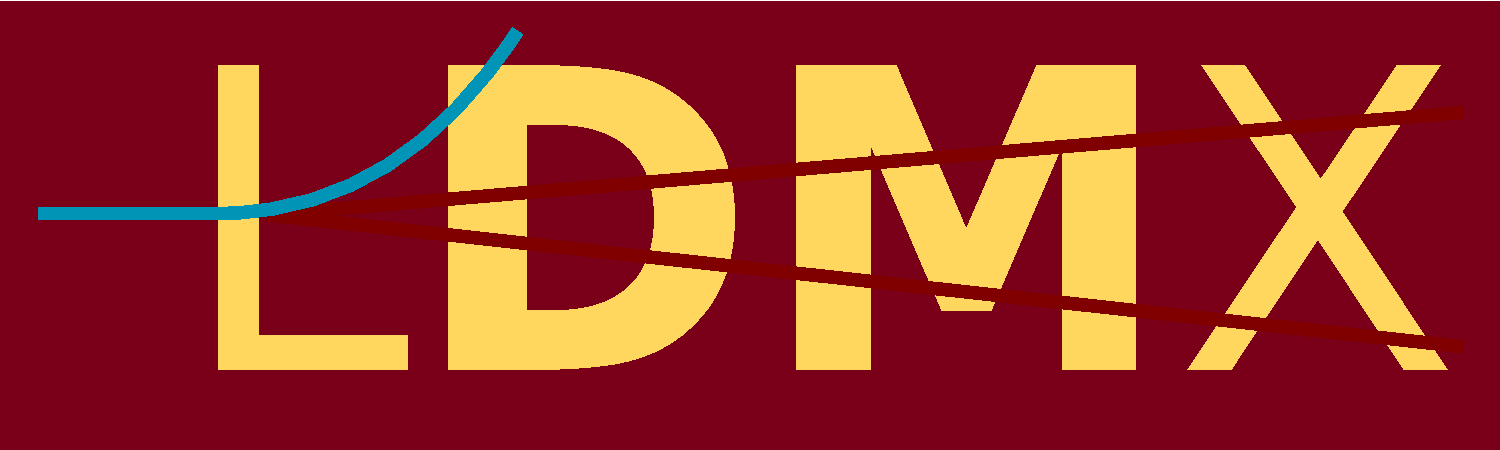
\includegraphics[height=0.95cm]{ldmx_logo}
      \end{textblock*}
      \begin{textblock*}{100mm}(0.7\textwidth,-0.95cm)
          
\includegraphics[height=0.95cm]{heavy_photon_logo}
      \end{textblock*}
  }

  % Beamer color definitions and palette
  %\setbeamercolor{structure}{fg=UMNStormy}
  \setbeamercolor{structure}{fg=UMNStormy} % Colors blocks and the 'Figure' caption heading. Default fg=UMNStormy.
  \setbeamercolor{palette primary}{fg=UMNMaroon, bg=UMNLightGray} % Default fg=UMNMaroon, bg=UMNLightGray.
  \setbeamercolor{palette secondary}{fg=UMNMaroon, bg=white}
  \setbeamercolor{palette tertiary}{fg=UMNLightGold, bg=UMNStormy}
  \setbeamercolor{frametitle}{fg=UMNLightGold, bg=UMNMaroon}
  \setbeamercolor{title}{fg=UMNMaroon, bg=UMNLightGray}
  \setbeamercolor{section in toc}{fg=UMNMaroon}
  \setbeamercolor{section in toc shaded}{fg=UMNMaroon}
  \setbeamercolor{button}{fg=UMNLightGold, bg=UMNMaroon}
  \setbeamercolor{palette sidebar secondary}{fg=UMNMaroon}
  \setbeamercolor{section in sidebar shaded}{fg=UMNMaroon}

  \setbeamertemplate{itemize item}{\color{UMNMaroon}$\blacksquare$}
  \setbeamertemplate{itemize subitem}{\color{UMNLightGold}$\blacktriangleright$}
  \setbeamertemplate{enumerate items}[default]
  \setbeamertemplate{sections/subsections in toc}[sections numbered]

  % Remove navigation symbols if not needed
  \setbeamertemplate{navigation symbols}{}

  \setbeamercolor{block body alerted}{fg=UMNSunny, bg=UMNMaroon!20}
  \setbeamercolor{block title alerted}{fg=UMNLightGold, bg=UMNMaroon}
}

%---------------------------------------------------------------------
% Author and Institution Details
%---------------------------------------------------------------------
\newcommand{\with}{} % Placeholder; fill or remove if not needed

\author{Billy Jackson} % Your name
\institute[UMN]{%
%  he/him/his \\[2mm]
  University of Minnesotas \\[2mm]
  \href{mailto:jack1851@umn.edu}{jack1851@umn.edu} \\[2mm]
  \begin{tabular}{p{0.4\textwidth}}\centering\with\end{tabular}
}

\usepackage{pgfpages}
\setbeamertemplate{note page}[plain]
\setbeameroption{show notes}
\addtobeamertemplate{note page}{}{\thispdfpagelabel{notes:\insertframenumber}}

\newcommand{\ssection}[1]{%
  \section{#1}%
  \sectionframe{#1}%
}%

\newenvironment{sframe}[1]{%
  \subsection{#1}%
  \begin{frame}{#1}%
}{%
  \end{frame}%
}%

\title[$\mathrm{W_R}$ Boson and Heavy Neutrino Search]{%
  Search for a Right-Handed W Boson and Heavy Neutrino of the Left-Right Symmetric Standard Model%
}

\begin{document}

\begin{frame}
  \maketitle
\end{frame}

\note[itemize]{
\item Hello everyone, for those of you who don't know me, my name is Billy.
  I am one of Jeremy's graduate students, and in this seminar I am going to
  talk about our search for a right-handed W boson and heavy neutrino of the 
  Left-Right Symmetric Standard Model. 
}

\begin{frame}{Outline}
  \begin{columns}
    \begin{column}{0.5\textwidth}
      \tableofcontents
    \end{column}
    \begin{column}{0.5\textwidth}
      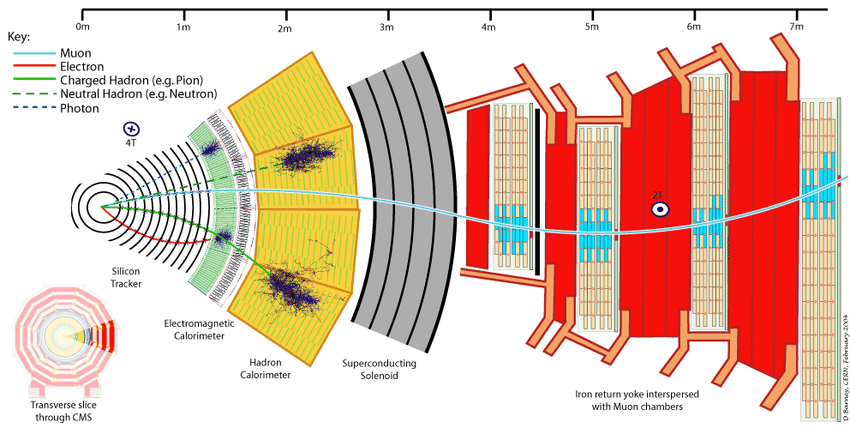
\includegraphics[width=0.9\textwidth]{../figures/experiment/cms-slice}
      \\
      \resizebox{0.9\textwidth}{!}{\begin{tikzpicture}
    \begin{feynman}
      %
      % -- Define the incoming quarks on the left
      \vertex (qbar) at (-2, 1.5) {\(\bar{q}'\)};
      \vertex (q)    at (-2,-1.5) {\(q\)};
      
      % -- Central vertex where q qbar' -> W_R
      \vertex [dot] (wr) at (0,0) {};
      
      % -- First decay: W_R -> N_\ell + l
      \vertex [dot] (Nl) at (2.5,0) {};
      \vertex (l1)  at (4,-1.5) {\(\ell^{+}\)};
      \vertex (N) at (4, 1.5) {};
      
      % -- Second decay: N_\ell -> l + W_R
      %    Then W_R -> 2 jets
      \vertex [dot] (wrl) at (4, 1.5) {};
      \vertex (l2) at (5.5,  3) {\(\ell^{-}\)};
      \vertex (wr2) at (6,  1) {};

      %    Then W_R -> 2 jets
      \vertex [dot] (jj) at (6, 1) {};
      \vertex (jet1) at (7.5,  1.7) {jet};
      \vertex (jet2) at (7.5, 0.3) {jet};
      
      % -- Draw the diagram
      \diagram*{
        % Incoming quarks
        (qbar) -- [fermion] (wr) -- [fermion] (q),
        
        % First decay of W_R
        (wr) -- [boson, edge label=\(W_R\)] (Nl),
        (l1) -- [fermion] (Nl),
        (Nl) -- [fermion, edge label=\(N_\ell\)] (wrl),
        
        % Decay of heavy neutrino N_l
        (wrl) -- [fermion] (l2),
        (wrl) -- [boson, edge label=\(W_R^{*}\)] (wr2),

        % Decay of second W_R into jets
        (jet1) -- [fermion] (jj) -- [fermion] (jet2),
      };
    \end{feynman}
  \end{tikzpicture}}
    \end{column}
  \end{columns}
\end{frame}

\ssection{Background}

\subsection{Parity Violation and Handedness}

\begin{frame}{Parity Violation in $\beta$ Decay}
  \begin{itemize}
    \item The parity operator $\hat{P}$ corresponds to a discrete 
      transformation $x \rightarrow -x$, etc.
    \item In 1957 C.S. Wu studied the beta decay:
      $\ce{^{60}_{27}Co \rightarrow ^{60}_{28}Ni + e^{-} + \bar{\nu_{e}}}$
  \end{itemize}
  \begin{columns}
    \begin{column}{0.65\textwidth}
      \begin{figure}
        \centering
        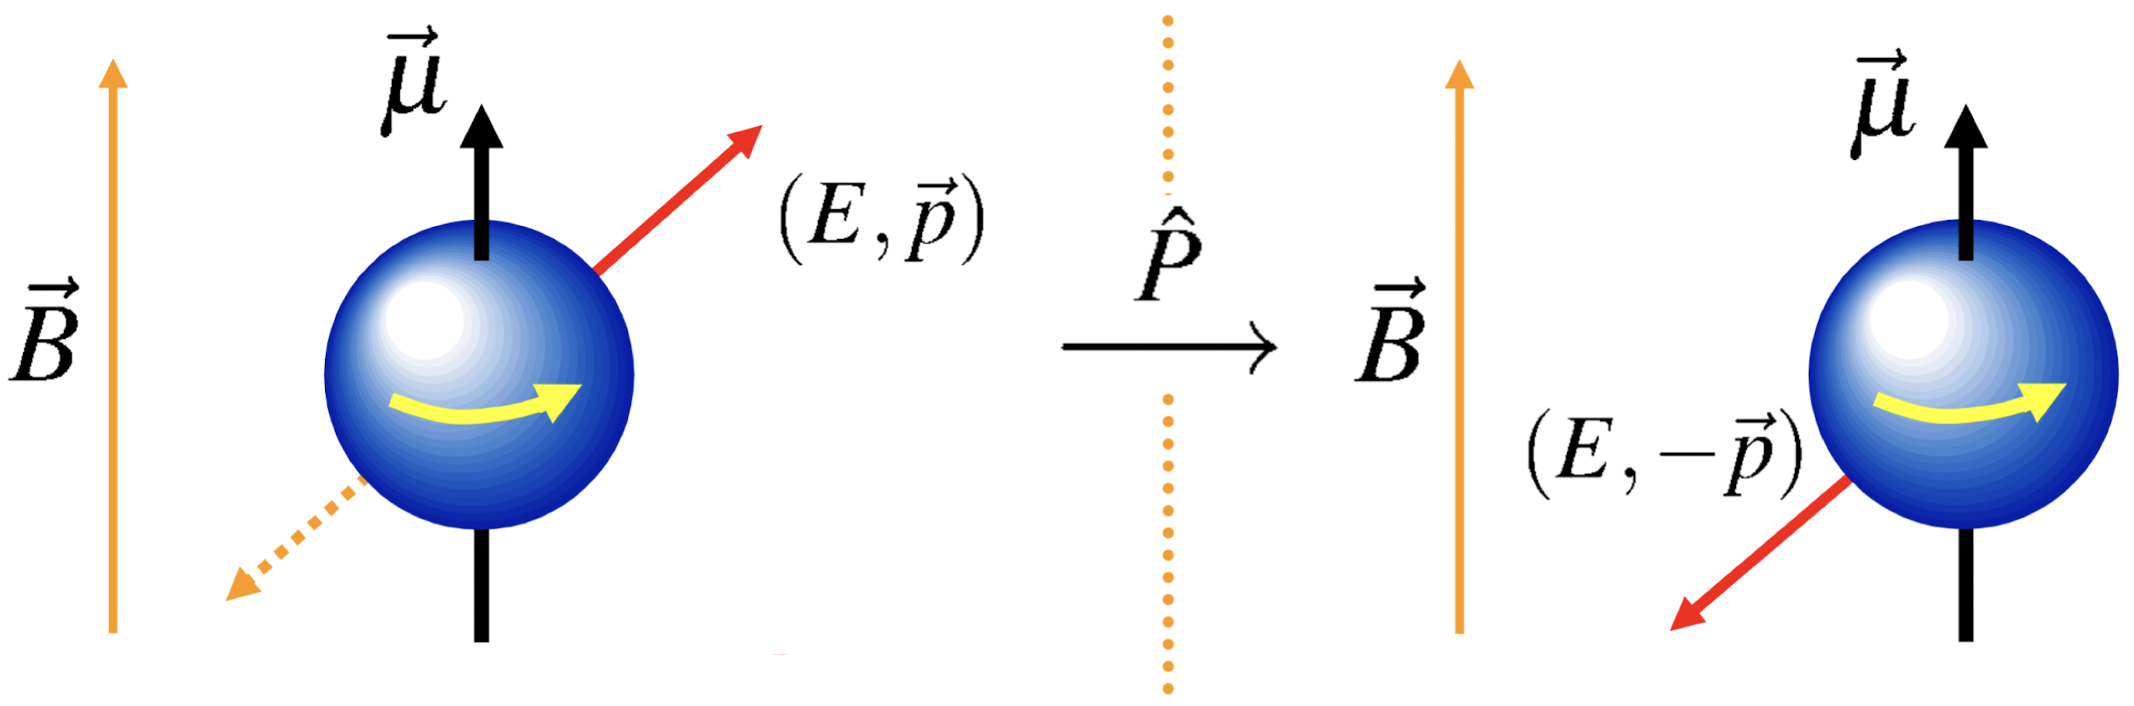
\includegraphics[width=\textwidth]{wu-experiment.png}
      \end{figure}
    \end{column}
    \begin{column}{0.3\textwidth}
      \begin{block}{}
        If parity were conserved: expect equal rate for producing $e^{-}$ in directions
            along and opposite to the nuclear spin.
      \end{block}
    \end{column}
  \end{columns}
  \begin{itemize}
    \item Observed \boldcol{UMNMaroon}{electrons emitted preferentially} in direction 
      opposite to applied field.
  \end{itemize}
  \begin{block}{}
    \centering
      Conclude \boldcol{UMNSunny}{parity is violated} in weak interactions.
  \end{block}
\end{frame}

\begin{frame}{Helicity States}
  \begin{block}{Definition}
    Define the \boldcol{UMNSunny}{Helicity} of a particle as the projection of its spin onto the direction of momentum.
  \end{block}
  \begin{columns}
    \begin{column}{0.60\textwidth}
      \begin{figure}
        \centering
        % MU DECAY - maximal positron energy
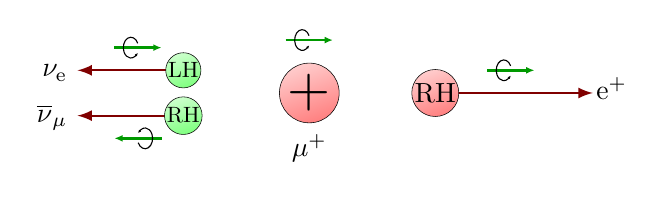
\begin{tikzpicture}[scale=2]
    % Local styling definitions
    \tikzset{>=latex} % set arrow head style
  
    % Color definitions
    \colorlet{vcol}{red!50!black}
    \colorlet{Scol}{green!60!black}
    
    % TikZ style definitions
    \tikzstyle{velocity}  =[->,thick,vcol]
    \tikzstyle{spin}      =[->,very thick,Scol]
    \tikzstyle{charge+}   =[very thin,draw=black,
                             top color=red!20!white, bottom color=red!50!white,
                             shading angle=20,circle,inner sep=0.2]
    \tikzstyle{charge0}   =[very thin,draw=black,
                             top color=green!20!white, bottom color=green!50!white,
                             shading angle=20,circle,inner sep=0.2]
  
    % Custom pic: spin (with a local length variable)
    \tikzset{
      pics/spin/.style={
        code={
          \def\Lspin{0.6} % Increased from 0.38 to 0.6 for longer spin arrows
          \draw[-{Latex[length=3,width=2.5]},pic actions,rotate=#1,line width=0.9,Scol]
            (-\Lspin/2,0) -- ++(\Lspin,0);
          \draw[pic actions,rotate=#1,thin,white]
            (-0.15*\Lspin,0) ++(170:{0.16*\Lspin} and {0.22*\Lspin}) arc (170:190:{0.16*\Lspin} and {0.22*\Lspin});
          \draw[-{Latex[length=1.2,width=1]},pic actions,rotate=#1,thin]
            (-0.15*\Lspin,0) ++(25:{0.16*\Lspin} and {0.22*\Lspin}) arc (25:305:{0.16*\Lspin} and {0.22*\Lspin})
            -- ++(50:0.09*\Lspin);
        }
      },
      pics/spin/.default=90,
    }
  
    % Drawing definitions
    \def\L{0.8}
    \def\v{1.2*\L}
    \coordinate (O) at (0,0);
    \coordinate (LT) at (-\L, 0.18*\L);
    \coordinate (LB) at (-\L,-0.18*\L);
    \coordinate (R) at (\L,0);
    \coordinate (T) at (0,0.42*\L);
    \coordinate (LTS) at ($(LT)+(-0.3*\v, 0.18*\L)$);
    \coordinate (LBS) at ($(LB)+(-0.3*\v,-0.18*\L)$);
    \coordinate (RS) at ($(R)+(0.50*\v,0.18*\L)$);
    
    % Vectors
    \draw[->,velocity] (R)++(0.05*\L,0) -- ++(\v,0);
    \draw[->,velocity] (LT) --++ (-0.7*\v,0) node[black,above=2,left=0] {\strut$\nu_\mathrm{e}$};
    \draw[->,velocity] (LB) --++ (-0.7*\v,0) node[black,below=3,left=0] {\strut$\overline{\nu}_\mu$};
    
    % Spin pictograms
    \pic at (RS)  {spin={  0}};
    \pic at (LTS) {spin={  0}};
    \pic at (LBS) {spin={180}};
    \pic at (T)   {spin={  0}};
    
    % Particles (black spin circles have been made larger)
    \draw[charge0] (LT) circle (0.1*\L); % Increased radius from 0.07*\L to 0.1*\L
    \draw[charge0] (LB) circle (0.1*\L); % Increased radius from 0.07*\L to 0.1*\L
    \node[charge+,scale=2] at (O) {$+$};
    \node[charge+,scale=1] at (R) {RH};
    \node[charge0,scale=0.80] at (LT) {LH};
    \node[charge0,scale=0.80] at (LB) {RH};
    \node at ($(O)+(0,-0.45*\L)$) {\strut$\mu^+$};
    \node[right=0] at ($(R)+(\v,0)$) {\strut$\mathrm{e}^+$};
    
\end{tikzpicture}
        \caption{Illustration of helicity states in muon decay. 
          $e^{+}$ and $\bar{\nu}_{\mu}$ are emitted as \boldcol{UMNMaroon}{right-handed} helicity states. 
          $\nu_e$ is emitted as a \boldcol{UMNMaroon}{left-handed} helicity state.}
      \end{figure}
    \end{column}
    \begin{column}{0.40\textwidth}
      \begin{block}{A Good Quantum Number}
        \centering
        $[\hat{H}_D, \hat{S} \cdot \hat{p}] = 0$
        \begin{itemize}
          \item Possible to find solutions of the Dirac equation which are also 
            eigenstates of Helicity.
        \end{itemize}
      \end{block}
    \end{column}
  \end{columns}
  \centering
  \boldcol{UMNSunny}{But it is important to remember that helicity is not Lorentz invariant.}
\end{frame}

\begin{frame}{Chirality}
  \begin{columns}
    \begin{column}{0.45\textwidth}
      \begin{figure}
        \centering
        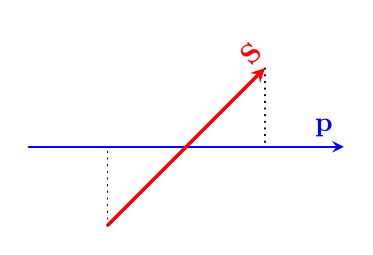
\begin{tikzpicture}[>=stealth, line cap=round, line join=round]

          % Define all coordinates (all non-negative)
          \coordinate (Foot) at (1,-1);   % "Foot" of the S arrow
          \coordinate (Tip)  at (3,1);     % "Tip"  of the S arrow
          \coordinate (Origin) at (0,0);   % Left end of the horizontal line
          \coordinate (EndLine) at (3.5,0);  % Right end of the horizontal line
          
          % Draw a horizontal reference line (no negative numbers)
          \draw[thick, blue] (Origin) -- (EndLine);
          
          % Draw the blue arrow for p to the right
          \draw[->, thick, blue] (EndLine) -- ++(0.5,0) node[midway, above] {\(\mathbf{p}\)};
          
          % Draw the red, thick diagonal arrow for S from Foot to Tip
          \draw[very thick, ->, red] (Foot) -- (Tip)
               node[pos=1, above, sloped] {\(\mathbf{S}\)};
               
          % Draw dotted vertical lines from the endpoints of S to the horizontal line at y = 0
          % Here we explicitly supply the coordinates
          \draw[dotted] (1,-1) -- (1,0);
          \draw[dotted] (3,1) -- (3,0);
        \end{tikzpicture}
        \caption{\footnotesize Reconstructed energy fraction separated by 
        energy going into nuclear processes.}
      \end{figure}
    \end{column}
    \begin{column}{0.55\textwidth}
      \begin{block}{Simulation Requirement}
        Electron reaches ECal with $> 87.5\%$ of the original beam energy.
      \end{block}

      Standard processes mimicking our signal are similar to thin-target analysis
      \begin{itemize}
        \item ``Nuclear'' processes (electrons and photons interacting with nuclei to produce hadrons)
        \item Muon pair production (via high-energy photon)
      \end{itemize}
    \end{column}
  \end{columns}
\end{frame}

\subsection{Left-Right Symmetric Extensions}

\begin{frame}{Charged Weak Interactions}
  \begin{columns}
    \begin{column}{0.5\textwidth}
      \begin{figure}
        \centering
        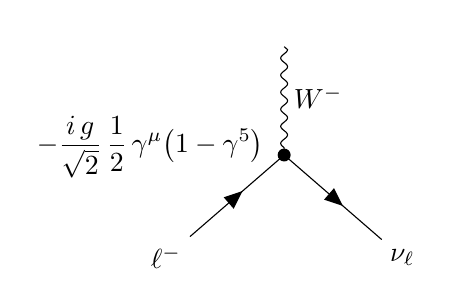
\begin{tikzpicture}
    \begin{feynman}
        % Define the central vertex and external particles
        \vertex [dot] (v) {};  % The central vertex
        \vertex [below left=1.3cm and 1.5cm of v]  (l) {\(\ell^-\)};
        \vertex [below right=1.3cm and 1.5cm of v] (n) {\(\nu_\ell\)};
        \vertex [above=1.5cm of v] (w) {};
    
        % Draw the diagram
        \diagram*{
          (l) -- [fermion] (v) -- [fermion] (n),
          (v) -- [boson, edge label'=\(W^-\)] (w),
        };
    
        % Place the vertex factor near the central vertex
        \node at ($(-1.7cm,0.1cm)$)
          {\(-\displaystyle \frac{i\,g}{\sqrt{2}} \,\frac{1}{2}\,\gamma^\mu \bigl(1-\gamma^5\bigr)\)};
    \end{feynman}
    \end{tikzpicture}
        \caption{The SM left-handed charged weak vertex.}
      \end{figure}
      \begin{itemize}
        \item The charged weak interaction vertex includes 
          the left-handed chiral projection operator.
        \item No theoretical explanation as to \emph{why} 
          the weak force is left-handed.
      \end{itemize}
    \end{column}
    \begin{column}{0.5\textwidth}
      \begin{figure}
        \centering
        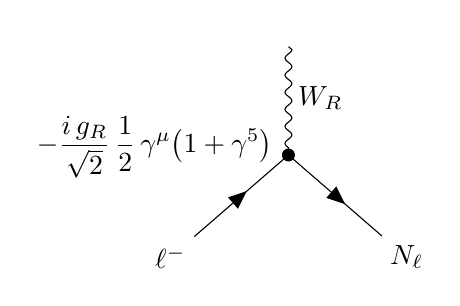
\begin{tikzpicture}
  \begin{feynman}
      % Define the central vertex and external particles
      \vertex [dot] (v) {};  % The central vertex
      \vertex [below left=1.3cm and 1.5cm of v]  (l) {\(\ell^-\)};
      \vertex [below right=1.3cm and 1.5cm of v] (n) {\(N_\ell\)};
      \vertex [above=1.5cm of v] (w) {};
  
      % Draw the diagram
      \diagram*{
        (l) -- [fermion] (v) -- [fermion] (n),
        (v) -- [boson, edge label'=\(W_{R}\)] (w),
      };
  
      % Place the vertex factor near the central vertex
      \node at ($(-1.7cm,0.1cm)$)
        {\(-\displaystyle \frac{i\,g_{R}}{\sqrt{2}} \,\frac{1}{2}\,\gamma^\mu \bigl(1+\gamma^5\bigr)\)};
  \end{feynman}
  \end{tikzpicture}
        \caption{The LRSM right-handed weak vertex.}
      \end{figure}
      \begin{itemize}
        \item Introduce $W_{R}^{\pm}$ bosons to mediate right
          chiral interactions.
      \end{itemize}
      \boldcol{UMNSunny}{The parity operator transforms left- and right-handed vertices into each other.}
    \end{column}
  \end{columns}
\end{frame}

\begin{frame}{Seesaw Mechanism}
  \begin{figure}
    \centering
    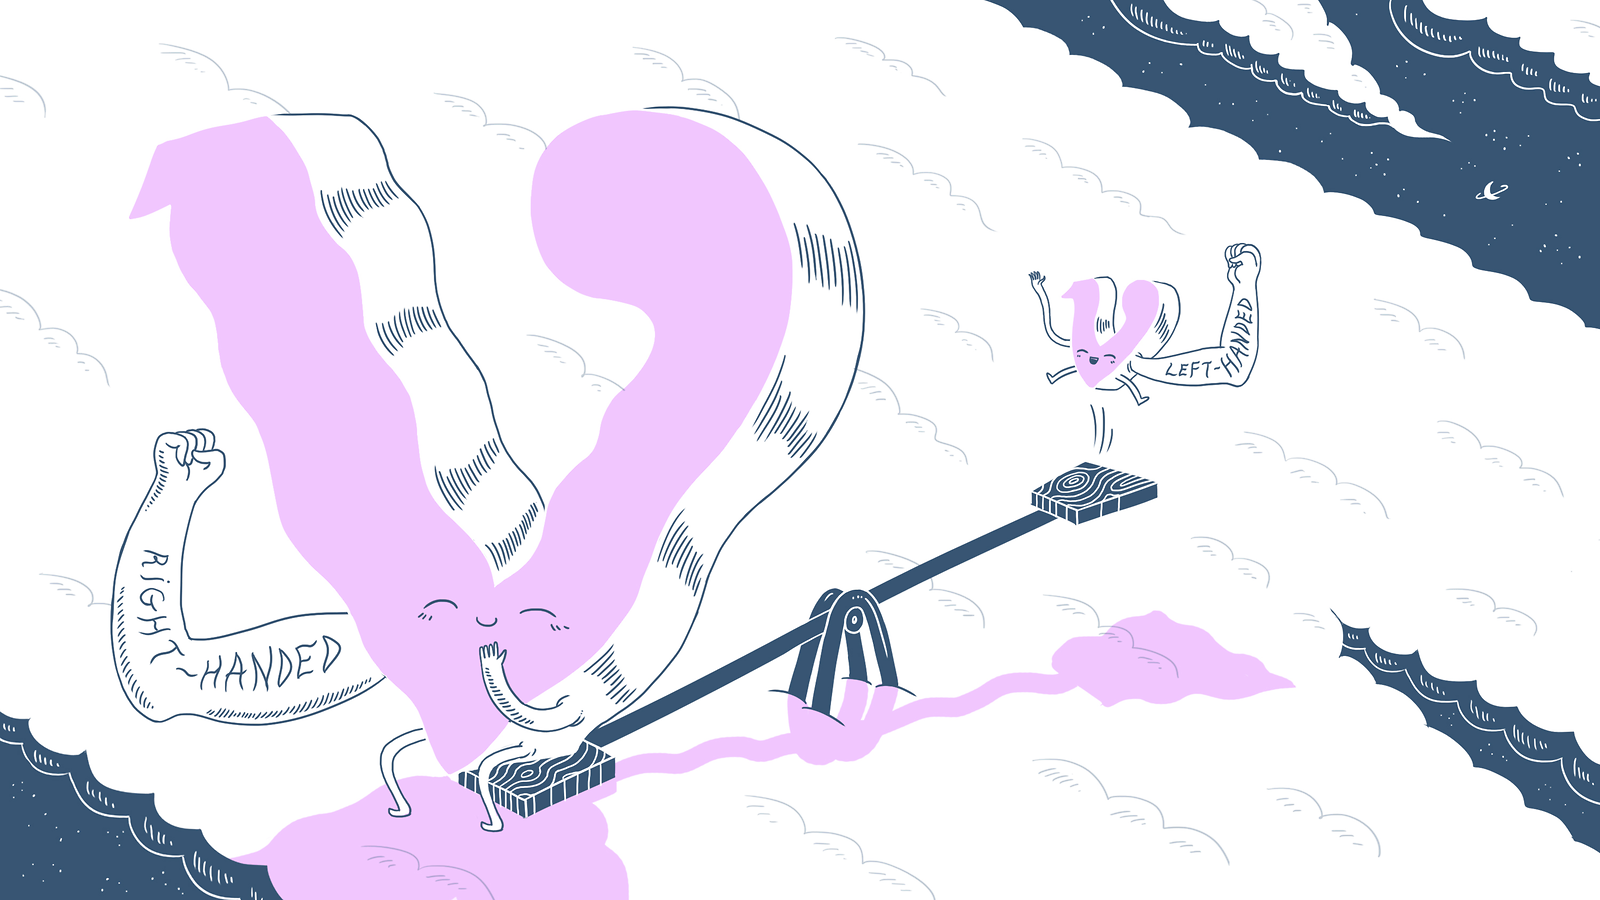
\includegraphics[width=0.70\textwidth]{seesaw-mechanism.png}
    \caption{In LRSM models the lightness of SM neutrinos is explained
    via the seesaw mechanism. Artwork by Sandbox Studio, Chicago with Ana Kova.}
  \end{figure}
\end{frame}

\begin{frame}{Left-Right Symmetric Model}
  \begin{block}{Postulate of Left-Right Symmetric Models}
    Parity violation is a low energy phenomenon -- 
    the result of a broken symmetry that is restored at a multi-TeV energy scale.
  \end{block}
  \vfill
  \begin{table}
    \begin{tabular}{|c|c|c|}
    \hline
    &&\\[-1em]
    ${}$ & Electroweak Standard Model & Left-Right Symmetric Model \\
    &&\\[-1em]
    \hline
    \hline
    &&\\[-1em]
    Gauge Group & $\mathrm{SU}(2)_{\mathbb{L}} \times \mathrm{U}(1)$ 
    & $\textcolor{red}{\mathrm{SU}(2)_{\mathbb{R}}} \times \mathrm{SU}(2)_\mathbb{L} 
    \times \mathrm{U}(1)$ \\ 
    &&\\[-1em]
    \hline
    &&\\[-1em]
    Fermions & 
    \(\begin{gathered}Q_{\mathbb{L}}=\left(u^i, d^i\right)_{\mathbb{L}}, 
        L_{\mathbb{L}}=\left(l^i, \nu^i\right)_{\mathbb{L}} \\ 
        Q_{\mathbb{R}}=\left(u^i, d^i\right)_{\mathbb{R}}, \quad  
        L_{\mathbb{R}}=l_{\mathbb{R}}^i\end{gathered}\) & 
        \(\begin{gathered}Q_{\mathbb{L}}=\left(u^i, d^i\right)_{\mathbb{L}}, 
        L_{\mathbb{L}}=\left(l^i, \nu^i\right)_{\mathbb{L}} \\ 
        Q_{\mathbb{R}}=\left(u^i, d^i\right)_{\mathbb{R}}, 
        L_{\mathbb{R}}=\left(l^i,\textcolor{red}{N^i}\right)_{\mathbb{R}} 
    \end{gathered}\) \\
    &&\\[-1em]
    \hline
    &&\\[-1em]
    Gauge Bosons & $W_{L}^{\pm}$, $Z$, $\gamma$ & $W_{L}^{\pm}$, 
    $\textcolor{red}{W_{R}^{\pm}}$, $Z$, $\textcolor{red}{Z^{\prime}}$ $\gamma$  \\
    \hline
\end{tabular}
    \caption{Summary of the Left-Right Symmetric SM
    with new extensions in \textcolor{red}{red}.}
  \end{table}
\end{frame}

\begin{frame}{Feynman Diagram}
  \begin{figure}
    \centering
    \begin{tikzpicture}
    \begin{feynman}
      %
      % -- Define the incoming quarks on the left
      \vertex (qbar) at (-2, 1.5) {\(\bar{q}'\)};
      \vertex (q)    at (-2,-1.5) {\(q\)};
      
      % -- Central vertex where q qbar' -> W_R
      \vertex [dot] (wr) at (0,0) {};
      
      % -- First decay: W_R -> N_\ell + l
      \vertex [dot] (Nl) at (2.5,0) {};
      \vertex (l1)  at (4,-1.5) {\(\ell^{+}\)};
      \vertex (N) at (4, 1.5) {};
      
      % -- Second decay: N_\ell -> l + W_R
      %    Then W_R -> 2 jets
      \vertex [dot] (wrl) at (4, 1.5) {};
      \vertex (l2) at (5.5,  3) {\(\ell^{-}\)};
      \vertex (wr2) at (6,  1) {};

      %    Then W_R -> 2 jets
      \vertex [dot] (jj) at (6, 1) {};
      \vertex (jet1) at (7.5,  1.7) {jet};
      \vertex (jet2) at (7.5, 0.3) {jet};
      
      % -- Draw the diagram
      \diagram*{
        % Incoming quarks
        (qbar) -- [fermion] (wr) -- [fermion] (q),
        
        % First decay of W_R
        (wr) -- [boson, edge label=\(W_R\)] (Nl),
        (l1) -- [fermion] (Nl),
        (Nl) -- [fermion, edge label=\(N_\ell\)] (wrl),
        
        % Decay of heavy neutrino N_l
        (wrl) -- [fermion] (l2),
        (wrl) -- [boson, edge label=\(W_R^{*}\)] (wr2),

        % Decay of second W_R into jets
        (jet1) -- [fermion] (jj) -- [fermion] (jet2),
      };
    \end{feynman}
  \end{tikzpicture}
    \caption{$\mathrm{W_R}$ decay chain. 
    The final state observables are two same-flavor leptons
    and two jets.}
  \end{figure}
\end{frame}

\note[itemize]{
  \item This feynmann diagram gives us a sense of what exactly we are looking for. 
  \item We have two qaurks coming in, annihilating and producing a right-handed W. 
  That right-handed W decays to a lepton and a heavy neutrino. That heavy neutrino 
  then decays back into a same flavor lepton and an off-shell right handed W, which 
  then decays into two quarks which hadronize to jets. 
  \item So, the observable objects in the decay are two same flavor leptons, and two jets. 
}

\ssection{LHC and CMS}

\begin{frame}{LHC}
  \begin{figure}
    \centering
    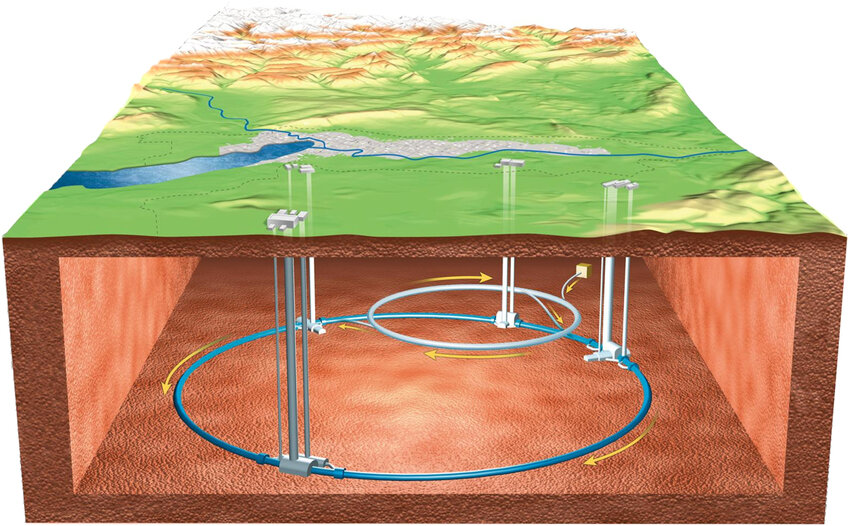
\includegraphics[width=0.7\textwidth]{../figures/experiment/lhc-schematic.png}
    \caption{Schematic showing the overall layout of the LHC. Image credit -- CERN.}
  \end{figure}
\end{frame}

\begin{frame}{CMS Detector}
  \begin{figure}
    \centering
    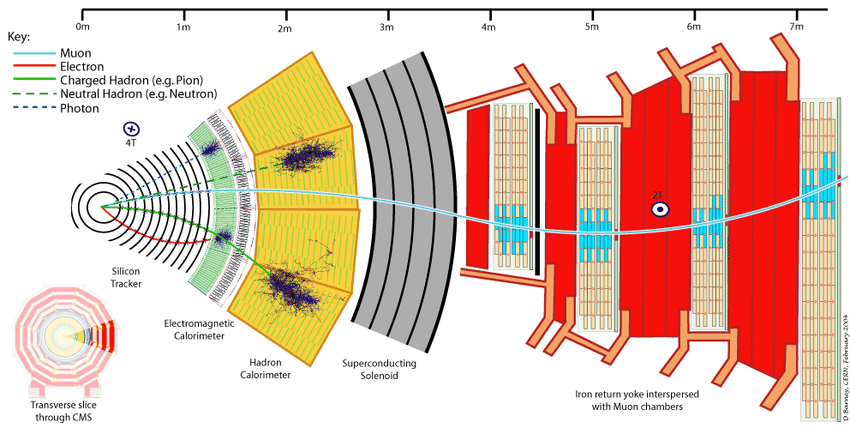
\includegraphics[width=0.85\textwidth]{../figures/experiment/cms-slice.png}
    \caption{CMS detector (slice view). Image credit -- CERN.}
  \end{figure}
\end{frame}

\begin{frame}{Analysis Regions}
  \begin{figure}
    \centering
    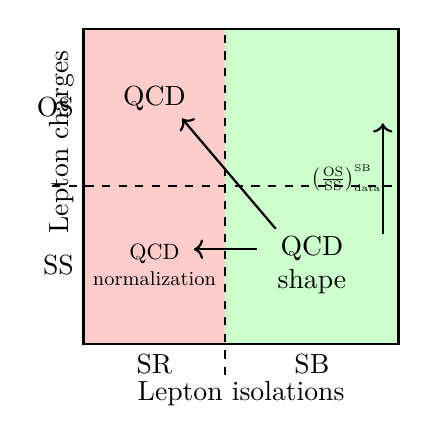
\begin{tikzpicture}[scale=4]
  
    \def\mx{0.45} %middle
    
    % boxes
    \fill [red!20!white] % SR
      (0,0) rectangle (\mx,1);
    \fill [green!20!white] % SB
      (\mx,0) rectangle (1,1);
    \draw[thick]
      (0,0) rectangle (1,1);
    
    % dashed lines
    \draw[dashed,thick]
      (\mx,-0.1) -- (\mx,1);
    \draw[dashed,thick]
      (-0.1,0.5) -- (1,0.5);
    
    % labels
    \draw
      (0,0.75) node[anchor=east]  {OS}
      (0,0.25) node[anchor=east]  {SS}
      (\mx/2,0) node[anchor=north] {SR}
      (0.5+\mx/2,0) node[anchor=north] {SB}
      (0,0.50) node[rotate=90,above=16pt] {Lepton charges}
      (0.50,0) node[below=10pt] {Lepton isolations};
    \draw
      (\mx/2,0.78) node {QCD}
      (0.5+\mx/2,0.25) node[align=center] {QCD\\shape} %{$\text{QCD}^\text{SS,SB}_\text{data}$};
      (\mx/2,0.25) node[align=center,scale=0.80] {QCD\\\small normalization};
    
    % arrows
    \draw[->,thick] % SR: SS -> OS
      (\mx+0.1,0.30) -- (\mx-0.1,0.30);
      %node[midway,above=8pt,right=-2pt,scale=0.70]{};
    \draw[->,thick] % SB: SS -> OS
      (0.95,0.35) -- (0.95,0.7)
      node[midway,above=8pt,left=-2pt,scale=0.70]{$\left(\frac{\text{OS}}{\text{SS}}\right)^\text{\tiny SB}_\text{\tiny data}$};
    
    \begin{scope}[shift={(\mx+0.02,0.54)},scale=0.35]
      \draw[->,thick]
        (0.40,-0.5) -- (-0.45,0.5);
        %node[midway,above=5pt,right=0pt,scale=0.8]{ $F^{\tiny \text{e}\mu}_\text{\tiny sim}$};
    \end{scope}
    
  \end{tikzpicture}
    \caption{A schematic diagram of the analysis region. The DY background is estimated from 
    the DY CR (blue).The backgrounds from $tW$ and $t\bar{t}$ production are estimated from the flavor CR 
    (green), where opposite flavor (OF) leptons are require.}
    \label{fig:dm-mass-scale}
  \end{figure}
\end{frame}

\note[itemize]{
  \item We define these different regions of phase space which we use to help estimate the backgrounds. 
  \item We estimate the backgrounds from Monte Carlo, but we use these different control regions in order to derive 
  corrections to the Monte Carlo in order to better predict the background in our Signal Region.
  \item We can see the Signal Region in the top right. The x-axis is the invariant mass of the two leptons in the final state. 
  So we require that the invariant mass of the two leptons by considerably high in order to reduce the background. 
  \item Moving to the left on the x-axis, you can see that if we lower that dilepton invariant mass requirement, 
  we get closer to the Z peak at 91.2 GeV. So we define a control region here, the Drell-Yan control region, right around 
  the Z peak because this is dominated by Drell-Yan and so we are able to drive corrections to our Drell-Yan Monte Carlo in 
  this control region. 
  \item Going back to our signal region and then moving down the y-axis, we see that in the signal region we require the leptons 
  to have the same flavor. But for ttbar events, the two tops are decaying independently, so they either can decay to the same flavor 
  or opposite flavor. So, when we require that our leptons be opposite flavor, we are in a region that is dominated by ttbar, and has 
  no signal within it either. So we are able to use this region to make more accurate corrections to our ttbar.
}

\begin{frame}{Standard Model}
  \begin{columns}
    \begin{column}{0.4\textwidth}
      \begin{figure}
        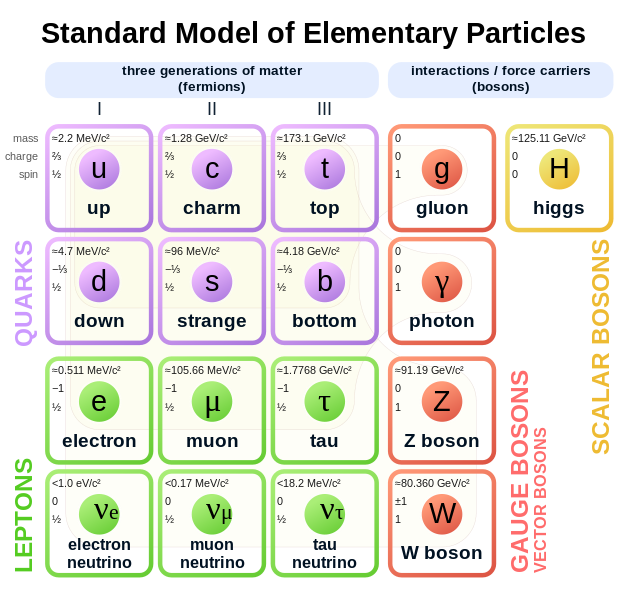
\includegraphics[width=\textwidth]{../figures/intro/Standard_Model_of_Elementary_Particles.svg.png}
        \caption{Credit to user Cush on wikipedia for providing this diagram.}
      \end{figure}
    \end{column}
    \begin{column}{0.6\textwidth}
      \begin{itemize}
        \item \boldcol{UMNSunny}{Law} -- summary of a set of consistent observations about phenomena
        \item \boldcol{UMNSunny}{Model} -- package of ``laws'' and their mathematical forms from which we can make predictions about future observations
        \item \boldcol{UMNSunny}{Orthogonal} -- used to emphasize that two different analyses are statistically independent
        \item \boldcol{UMNSunny}{Event} -- a piece of data (one ``row'' of our data ``table''), a short period of time around a single electron entering the detector volume
      \end{itemize}
    \end{column}
  \end{columns}
\end{frame}

\note[itemize]{
\item Laws are summaries of observations and models
  are just packaging these laws with some mathematical sugar
\item The SM is the most quantitatively accurate physics model ever known to human kind.
\item It is a package of particles and their interactions (also represented by particles)
  from which we can -- with a specific mathematical framework -- make predictions about
  our observations.
\item \textbf{BUT} it fails to account for all observed phenomena (e.g. \emph{gravity})
\item Other vocabulary that is helpful to know...
}

\begin{frame}{Particle Mixing}
  \begin{columns}
    \begin{column}{0.4\textwidth}
      \begin{figure}
        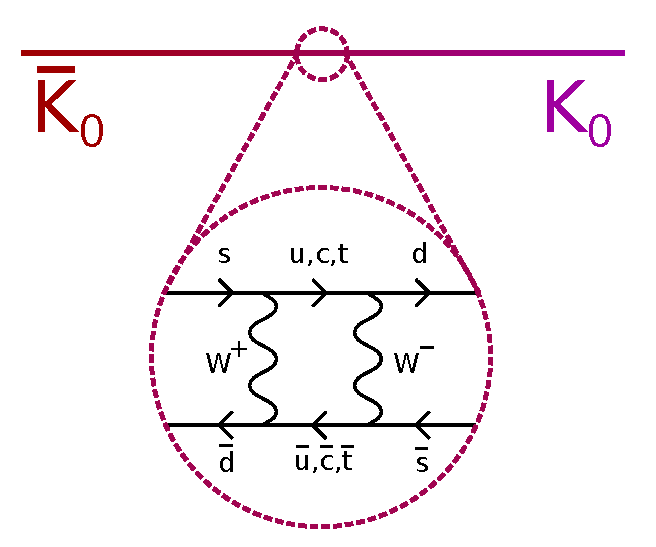
\includegraphics[width=\textwidth]{%
          ../figures/intro/Kaon-box-diagram-with-bar.pdf%
        }
        \caption{Figure created by user NikNaks on Wikipedia.}
      \end{figure}
    \end{column}
    \begin{column}{0.6\textwidth}
      Observations of particles ``changing'' into other particles with some probability
      (like neutral kaons).
      \begin{itemize}
        \item With quark model, we can describe this mixing with a Feynman diagram
        \item But also, at lower energies, we can just represent this process with
          an effective vertex
      \end{itemize}
    \end{column}
  \end{columns}
\end{frame}

\note[itemize]{
\item The quantum nature of the Standard Model leads to some odd behavior
\item One odd behavior is this idea of mixing where, from a certain perspective,
  particles ``change'' into other particles with some probability
\item We observe this ``mixing'' in systems like the neutral kaon which mixes
  with its own anti-particle
\item The quarks from the SM offer an explanation (via the lower Feynman diagram)
  that does quantitatively align with measurements
\item However, we can also just treat this detailed Feynman diagram as an effective
  vertex between the two kaons -- helpful if we are at lower energies where we only
  are observing the kaons themselves
}

\begin{frame}{Displaced Decay Vertices}
  \begin{columns}
    \begin{column}{0.8\textwidth}
      \begin{figure}
        \begin{tikzimage}[0.6\textwidth]{../figures/intro/bubble-chamber.jpeg}
          \definecolor{brilliantrose}{rgb}{1.0, 0.33, 0.64}
          % \draw[step=0.1,black,thin] (0.0,0.0) grid (1.0,1.0);
          \node (prod) at (0.4,0.54) {};
          \node[circle,draw=brilliantrose] (decay) at (0.515,0.54) {};
          \draw[dashed,brilliantrose,thick] (prod) -- (decay);
      
          \node (beam1) at (0.1,0.5) {\color{brilliantrose}\(\pi^-\)};
          \node (beam2) at (0.2,0.5) {};
          \draw[->,brilliantrose,thick] (beam1) -- (beam2);
        \end{tikzimage}
        \caption{Image of CERN's first liquid hydrogen bubble chamber from 1960.}
      \end{figure}
    \end{column}
  \end{columns}
\end{frame}

\note[itemize]{
\item Our particle detectors are not perfect and they cannot detect all particles
\item This leads to particles appearing to appear out of nowhere
\item Particles our detector cannot see (for example, the neutral $\Lambda$ does not leave a track here)
  then decay into particles we can see leading to a ``displaced vertex''
}

\begin{frame}{Dark Matter}
  \begin{columns}
    \begin{column}{0.5\textwidth}
      \begin{figure}
        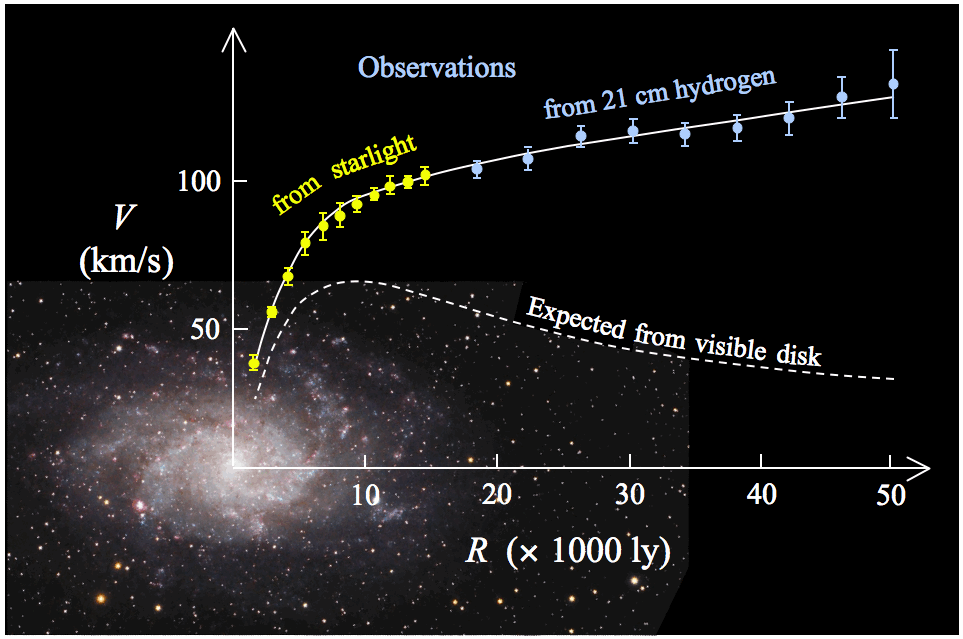
\includegraphics[width=\textwidth]{../figures/theory/rotation-curve-evidence-for-dm.png}
        \caption{Stuff is spinning too fast!}
      \end{figure}
    \end{column}
    \begin{column}{0.5\textwidth}
      \begin{figure}
        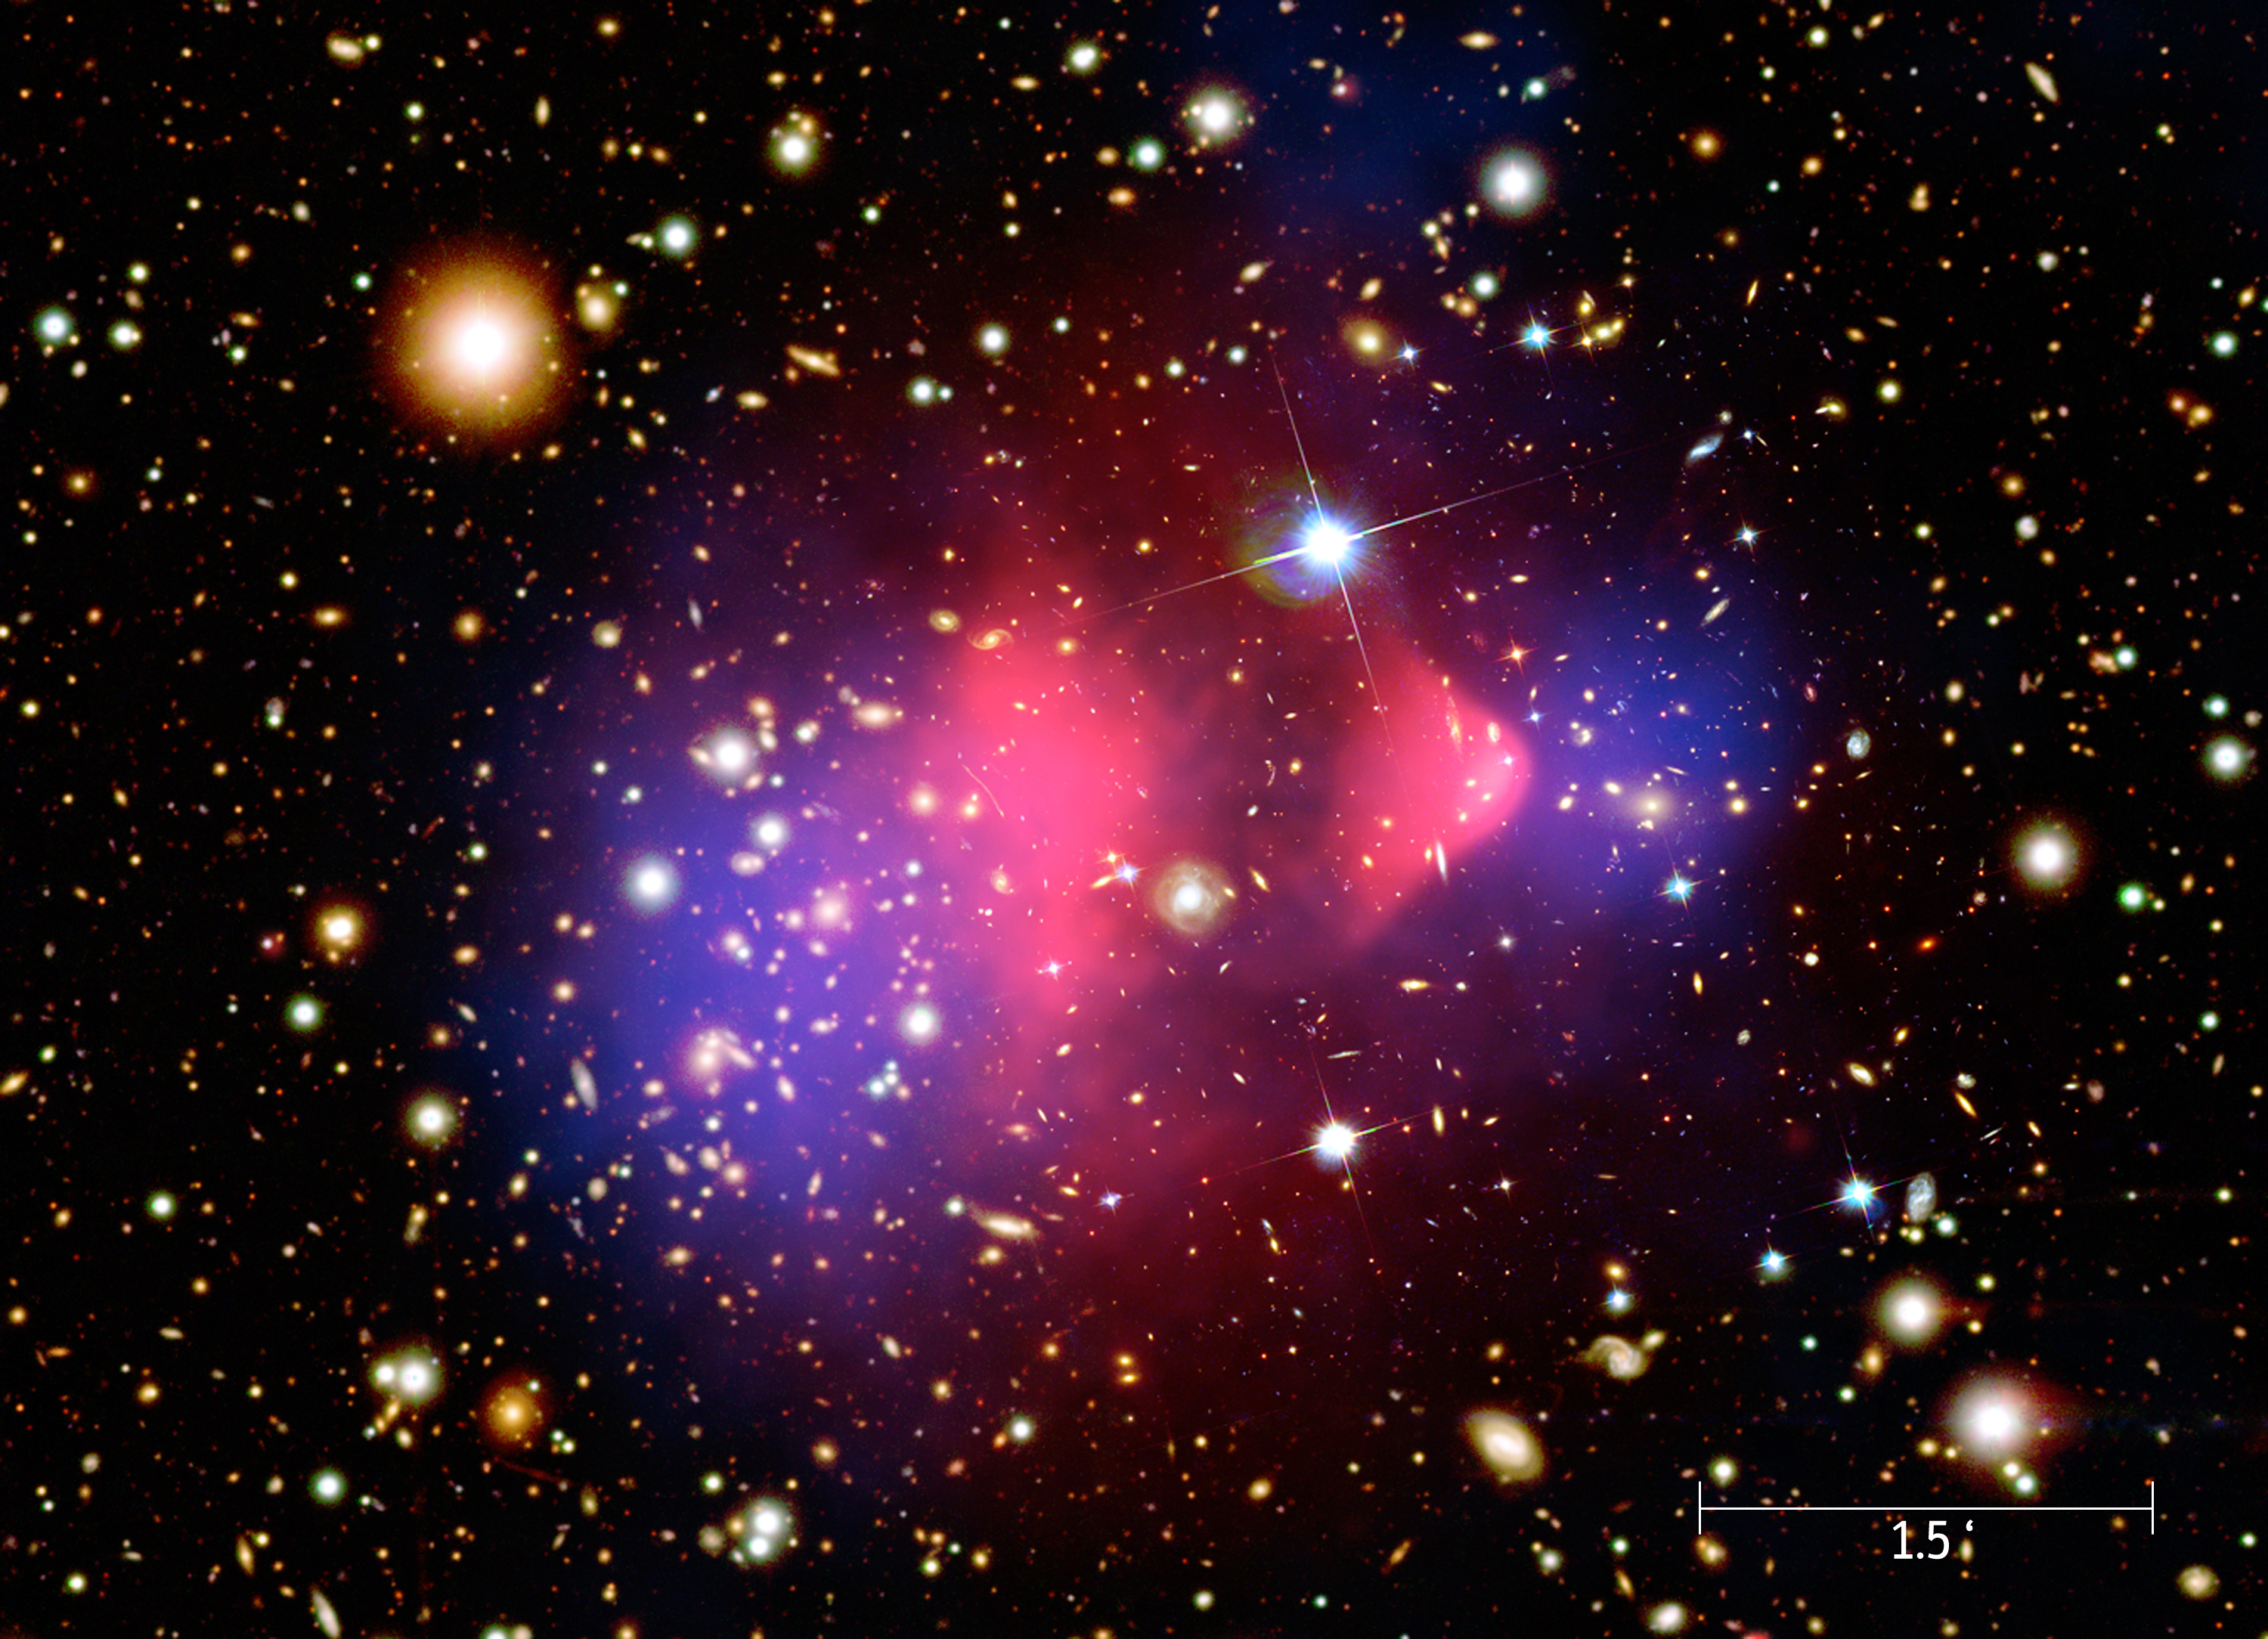
\includegraphics[width=\textwidth]{%
          ../figures/intro/bullet-cluster.jpg
        }
        \caption{Gravitational lensing (blue) and infrared (pink) observations
        show mass in different places!}
      \end{figure}
    \end{column}
  \end{columns}
\end{frame}

\note[itemize]{
\item One of the phenomena the SM doesn't account for is DM
\item We know it exists
\item Galactic rotation curves
  \begin{itemize}
    \item Expected from visible matter in dashed line
    \item Observed yellow/blue data points
    \item Either more matter we can't see helping hold these stars
      in or our model of gravity is wrong
  \end{itemize}
\item Grav lensing
  \begin{itemize}
    \item Very confident our model of gravity is correct from other measurements
    \item Additionally, grav lensing data of the bullet cluster
    \item Infrared signals (pink) differ in location than grav lensing (blue)
    \item ``heavy'' matter separate from ``visible'' matter
  \end{itemize}
}

\begin{frame}{Thermal Relic Dark Matter}
  \begin{block}{Narrow Wealth of Possibilities}
    Make the simple assumption that \ac{dm} has always been here.
  \end{block}
  \vfill
  \begin{figure}
    \centering
    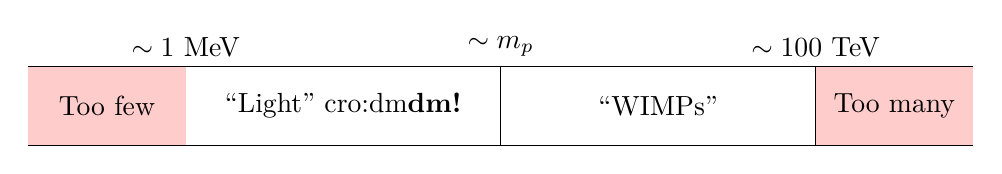
\begin{tikzpicture}
  % horizontal top/bottom lines
  \draw (0,0) -- (12,0);
  \draw (0,1) -- (12,1);
  % dividing lines along with relevant scale markers
  \draw (2,0) -- (2,1) node[above] {$\sim 1~$MeV};
  \draw (6,0) -- (6,1) node[above] {$\sim m_p$};
  \draw (10,0) -- (10,1) node[above] {$\sim100~$TeV};
  % fill non-thermal ranges with light red
  \fill [red!20!white] (0,0) rectangle (2,1);
  \fill [red!20!white] (10,0) rectangle (12,1);
  % labels offering descriptions of ranges inside the boxes
  \node at (1,0.5) {Too few};
  \node at (4,0.5) {``Light'' \acs{dm}};
  \node at (8,0.5) {``WIMPs''};
  \node at (11,0.5) {Too many};
\end{tikzpicture}

    \caption{Mass scale of Thermal Relic \ac{dm}.
      The regions in red are excluded by applying the thermal relic assumption
      to our observations of the universe's early evolution.}
    \label{fig:dm-mass-scale}
  \end{figure}
  \boldcol{UMNSunny}{Both LDMX and HPS are searching for production of Light DM with electrons.}
\end{frame}

\note[itemize]{
\item Simplifying assumption: Dark Matter has always been here (like standard matter)
  and was in thermal equilibrium with standard matter in the early universe
\item (Observations of the CMB also imply this so its a decently motivated assumption.)
\item Limits the scale of mass of DM particles by connecting the mass to the interaction
  strength
\item Above $m_p\sim\qty{1}{\GeV}$, the interaction could be provided by the standard Weak
  force (so-called WIMPs), many experiments searching in this region
\item Below $m_p$, the interaction needs to be even weaker than the standard Weak force
\item Particles are lighter than WIMPs so referred to as Light DM
}

\begin{frame}{A Benchmark Model}
  \begin{columns}
    \begin{column}{0.5\textwidth}
      \begin{figure}
        \centering
        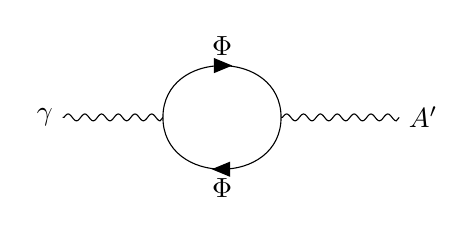
\begin{tikzpicture}
  \begin{feynman}
    \vertex (standard) {\(\gamma\)};
    \vertex [right=of standard] (loopleft);
    \vertex [right=of loopleft] (loopright);
    \vertex [right=of loopright] (dark) {\(A'\)};

    \diagram*{
    (standard)
    -- [photon] (loopleft)
    -- [fermion, half left, edge label=\(\Phi\)] (loopright)
    -- [photon] (dark),
    (loopright)
    -- [fermion, half left, edge label=\(\Phi\)] (loopleft),
    };
  \end{feynman}
\end{tikzpicture}

        \caption{Heavy field $\Phi$ enabling mixing between standard and dark photons.}
      \end{figure}

      The required connection between standard and dark sector provides an
      effective mixing of the standard and dark photons at our energy scales.
    \end{column}
    \begin{column}{0.5\textwidth}
      \begin{figure}
        \centering
        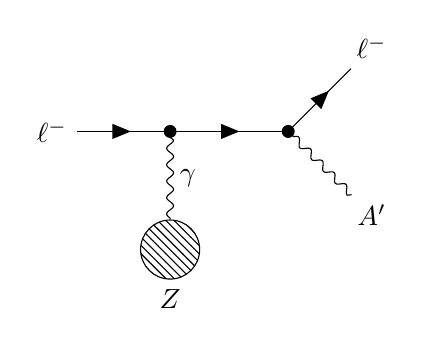
\begin{tikzpicture}
  \begin{feynman}
    \vertex (in) {\(\ell^-\)};
    \vertex [right=of in, dot] (nuc) {};
    \vertex [below=of nuc, blob, label={below:\(Z\)}] (nucleus) {};
    \vertex [right=of nuc, dot] (emit) {};
    \vertex [above right=of emit] (recoil) {\(\ell^-\)};
    \vertex [below right=of emit] (decay) {\(A'\)};
    % \vertex [above right=of decay] (chi2) {\(\overline{\chi}\)};
    % \vertex [below right=of decay] (chi1) {\(\chi\)};

    \diagram*{
    (in) -- [fermion] (nuc) -- [fermion] (emit) -- [fermion] (recoil),
    (nucleus) -- [photon, edge label'=\(\gamma\)] (nuc),
    (emit) -- [photon] (decay),
    % (emit) -- [photon, edge label'=\(A'\)] (decay),
    % (chi2) -- [fermion] (decay) -- [fermion] (chi1),
    };
  \end{feynman}
\end{tikzpicture}

        \caption{Dark bremsstrahlung process.}
      \end{figure}
      
      Mixing allows for a new process producing dark particles

      \boldcol{UMNSunny}{Both HPS and LDMX search for this production mechanism}
    \end{column}
  \end{columns}
\end{frame}

\note[itemize]{
\item The thermal relic assumption combined with curiosity for the lower masses
  requires the introduction of a new field which is presumably much heavier
  (i.e. harder to produce and observe) than our current energies.
\item This required connection does provide an effictive mixing of the standard
  and dark photons (like how kaons can mix) at our energy scales
\item Allowing for this mixing then gives a new process that can produce
  dark particles in our experiments -- dark bremsstrahlung
\item Both HPS and LDMX search for dark brem; however, they have different
  tactics to look for it
}

\ssection{Search Strategy}

\note[itemize]{
\item First, let's talk about the experiment I started with
\item The Light Dark Matter eXperiment is a \textbf{Missing Momentum} search for
  the dark bremsstralung production of dark particles with an electron beam
\item i.e. We assume that the dark photon that is produced ``stays in'' the dark sector
  and the momentum it had is not observable by our detector
}

\subsection{Resonance Searches}

\subsection{Analysis Regions}
\begin{frame}{Missing Momentum Search}
  \begin{columns}
    \begin{column}{0.25\textwidth}
      \begin{block}{To Do MM Search}
        \begin{itemize}
          \item Know fate of every single electron
          \item Need faithful ID of even very rare SM processes
        \end{itemize}
      \end{block}
    \end{column}
    \begin{column}{0.7\textwidth}
      \begin{figure}
        \centering
        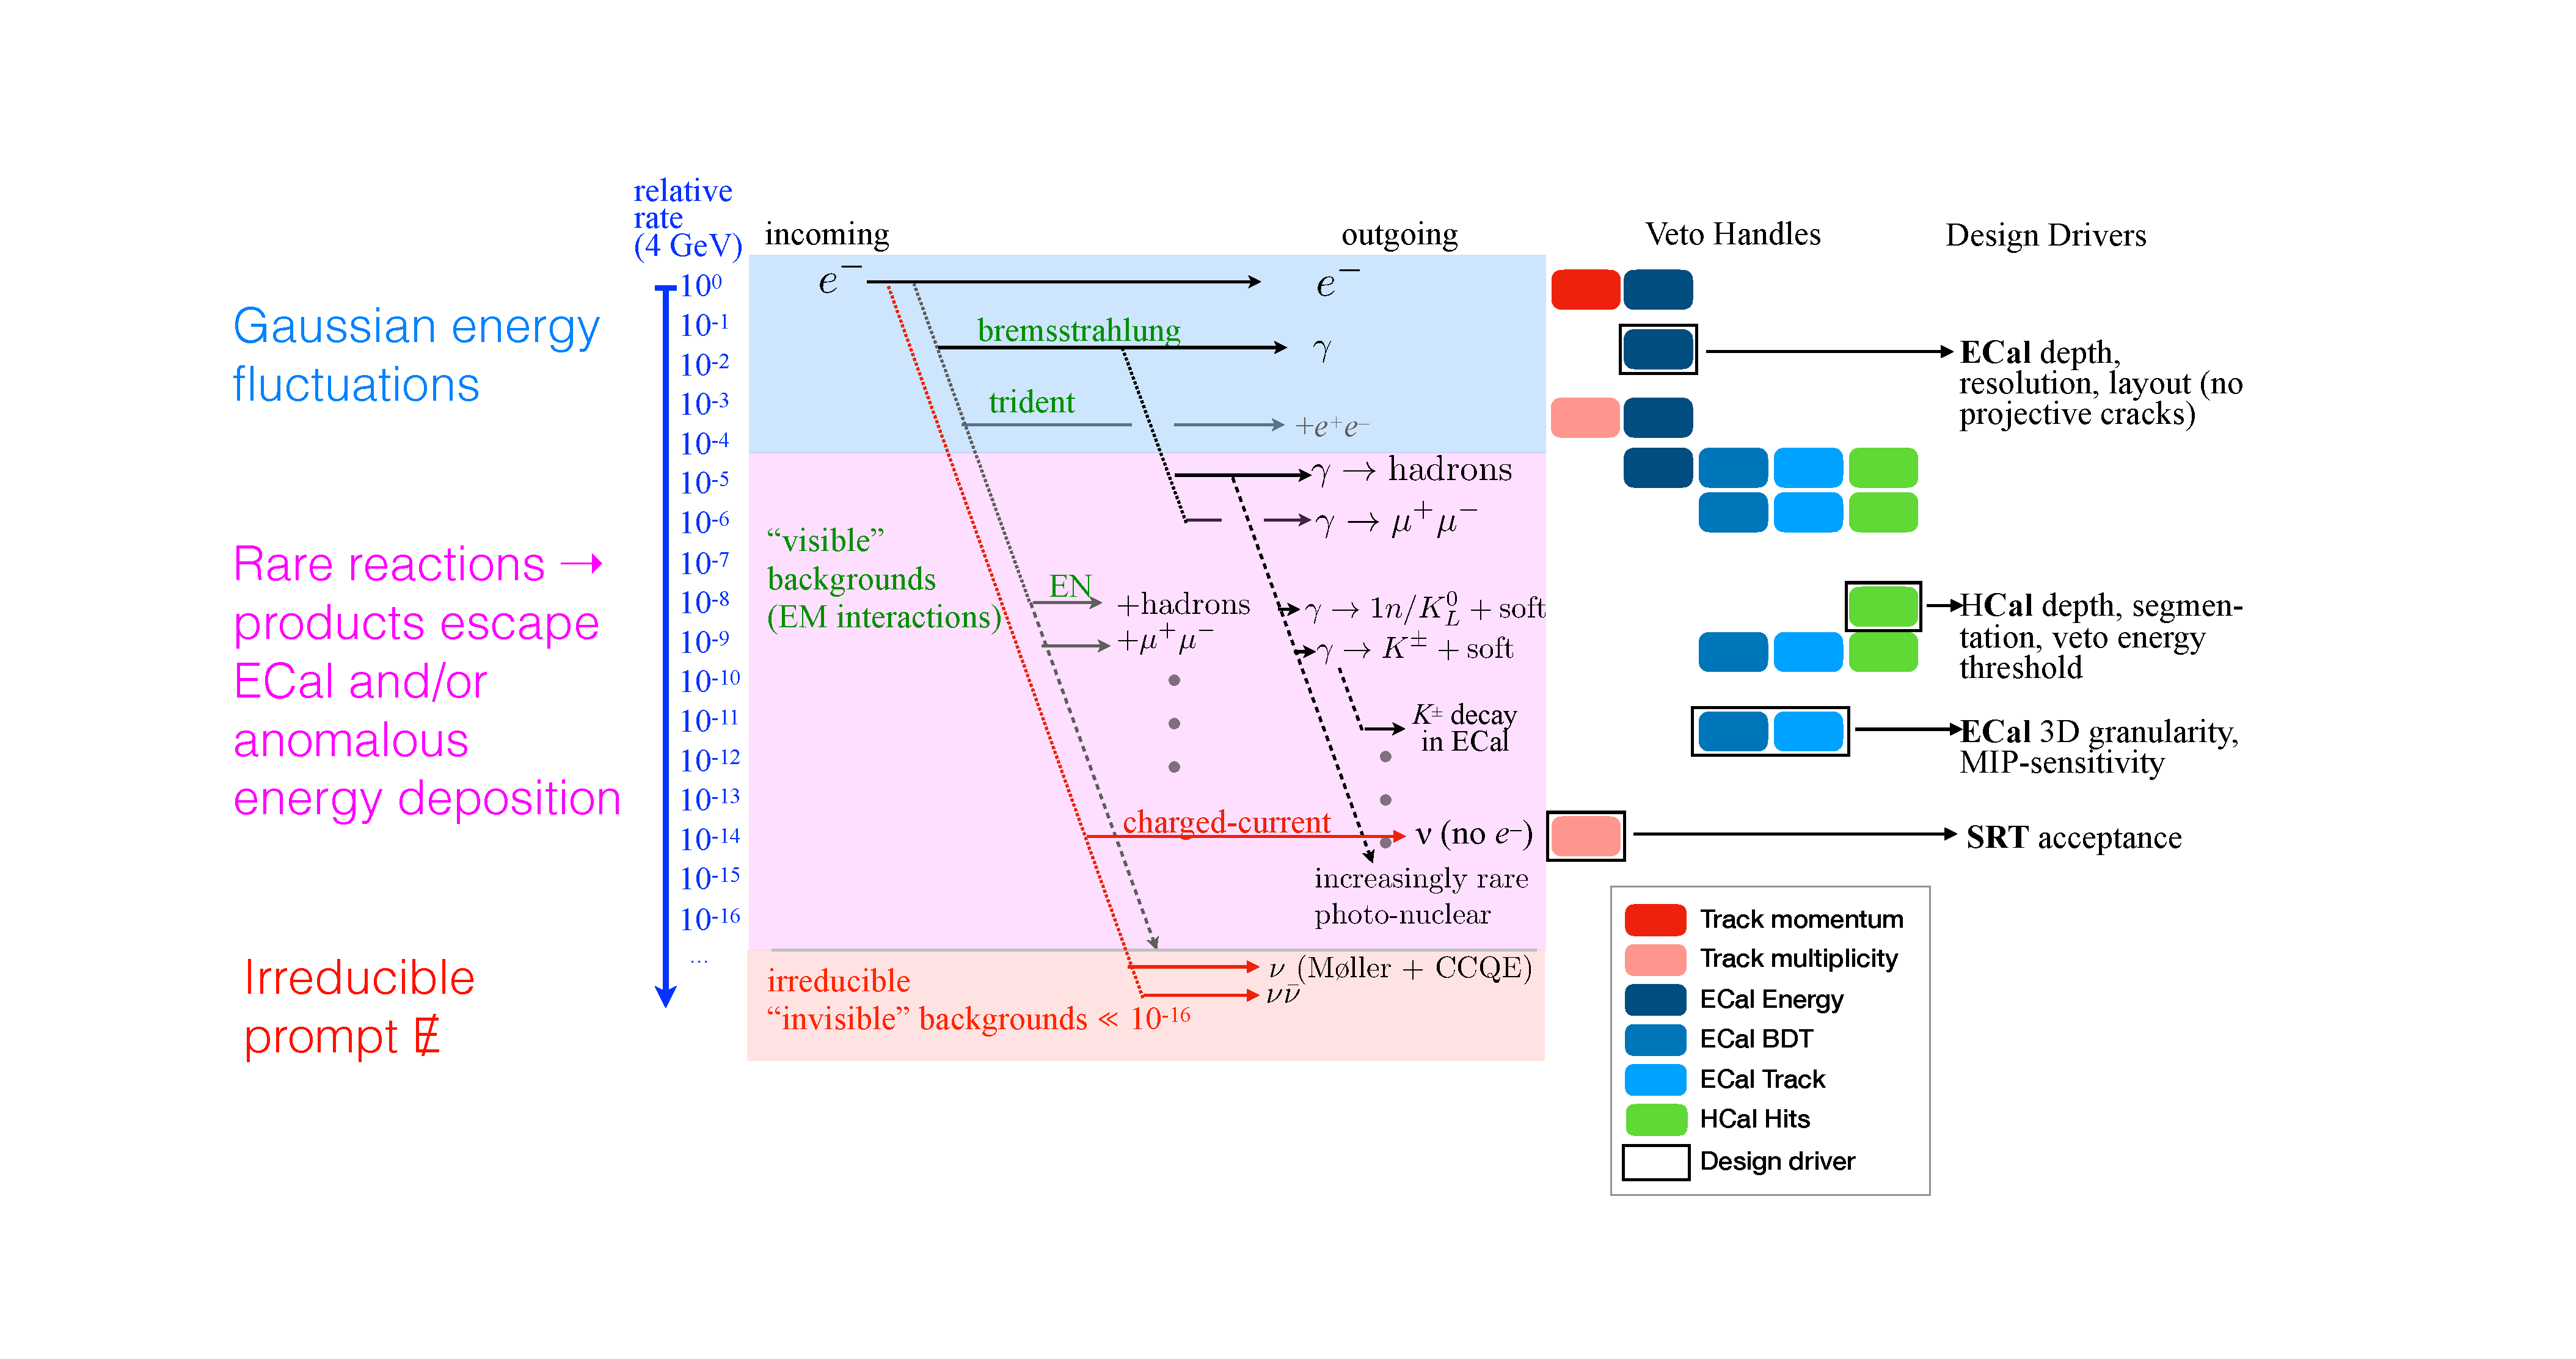
\includegraphics[width=\textwidth]{../figures/ldmx/experiment/reaction_staircase_with_designDrivers.pdf}
        \caption{Credit to Tim Nelson}
      \end{figure}
    \end{column}
  \end{columns}
\end{frame}

\note[itemize]{
\item LDMX, as mentioned, is a MM search and, to do MM, we need to
  know the fate of \textbf{every single electron}
  and be able to faithfully ID very rare SM processes
\item Here is a diagram of prominent SM processes ordered by their relative rate
\item Blue -- would happen in any target "brem" and "trident"
  \begin{itemize}
    \item Need tracker to measure incident and outgoing momenta of electron
    \item Need ECal to measure photon if brem ocurs
  \end{itemize}
\item Pink -- sometimes the photon gets up to some funky stuff in the ECal
  that makes the ECal's measurement more complicated
  \begin{itemize}
    \item rarer processes requiring more granular information about what happens
    \item stuff that is hard for the ECal to measure motivates a seconadary
      calorimeter for these particles (HCal)
  \end{itemize}
\item Red -- very rare processes that we will not be able to remove
  (but could constrain using measurements of these processes by other experiments)
}

\begin{frame}{Experiment}
  \begin{figure}
    \centering
    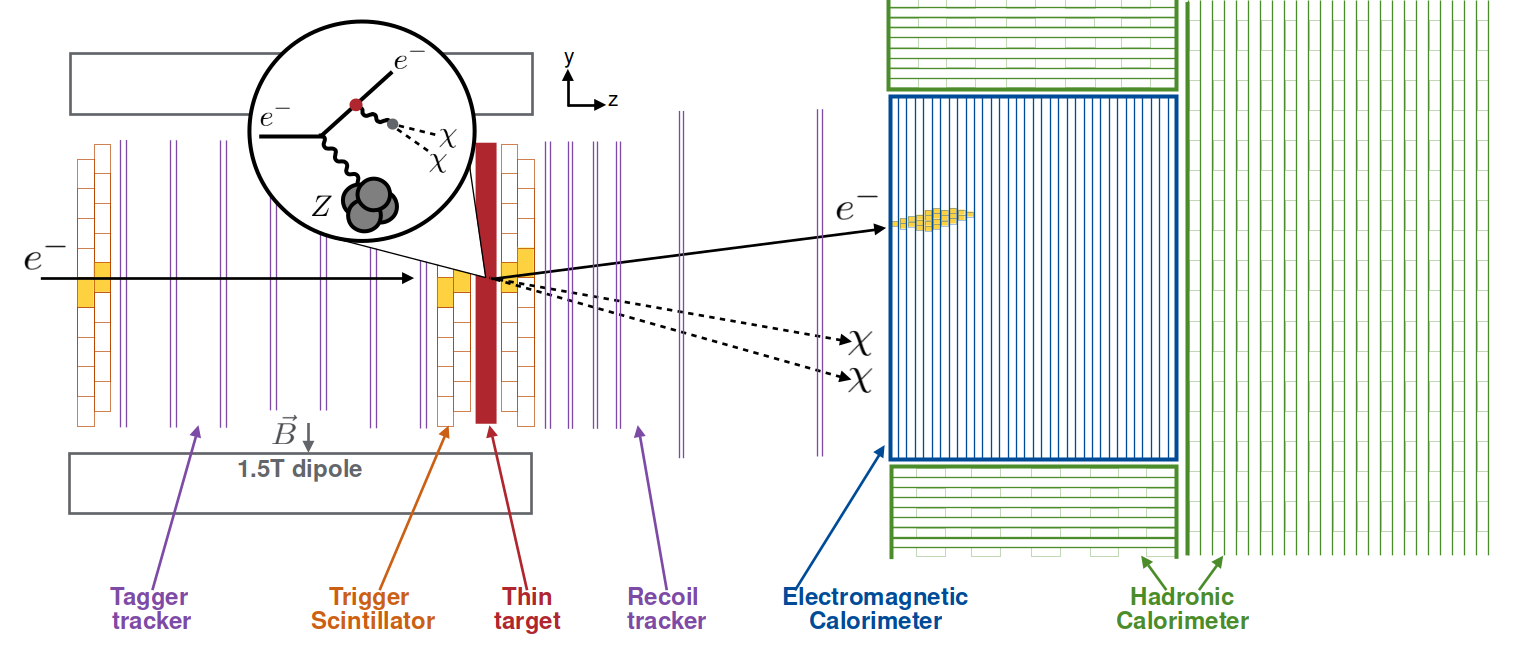
\includegraphics[width=\textwidth]{../figures/ldmx/experiment/detector.png}
    \caption{Credit to Christian Herwig for original diagram}
  \end{figure}
\end{frame}

\note[itemize]{
\item These processes motivate a staged design
  \begin{itemize}
    \item a tracker (tagger for incoming and recoil for outgoing)
    \item ECal for electrons/positrons and photons
    \item HCal for hadrons (e.g. protons/neutrons) and muons
    \item a TrigScint to quickly count electrons and help ECal make trigger decision in time.
  \end{itemize}
\item Hosted at SLAC Natl Accelerator Lab, recieving beam from LCLS-II 
\item Beam facility upgrading from \qty{4}{\GeV} to \qty{8}{\GeV}, LDMX may see
  some \qty{4}{\GeV} beam depending on how schedules line up but a majority
  of data will be taken with \qty{8}{\GeV}
\item \textbf{Thin target to help momentum resolution.} -- most electrons pass through
  only minimally interacting
\item Can we still use this data we would collect anyways?
}

\begin{frame}{Using the ECal as Target}
  \begin{figure}
    \centering
    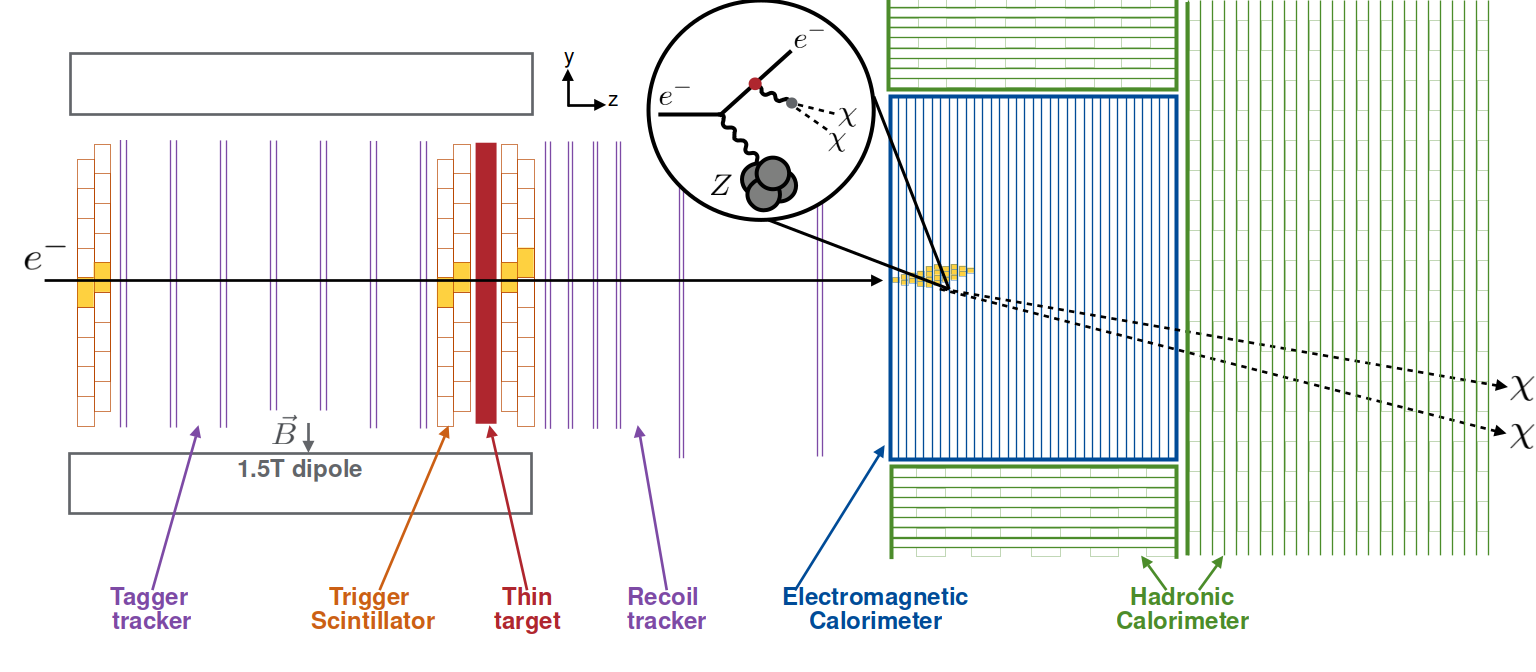
\includegraphics[width=\textwidth]{figs/detector-eat-signal.png}
    \caption{Credit to Christian Herwig for original diagram}
  \end{figure}
\end{frame}

\note[itemize]{
\item Yes we can!
\item If the dark brem process exists and would happen in the thin target,
  it would also happen within other parts of our detector -- namely the ECal
  which has a lot of material and would recieve similar numbers of electrons as
  the target
\item Use the Ecal as another Target for our dark brem search
\item Shift focus to \textbf{Missing Energy} search
\item Use upstream detectors to confirm near-beam-energy electron entering ECal \\
  (orthogonality condition, MM search requires significant loss within thin target)
\item ECal has more material $\to$ more ``chances'' for dark brem to happen \\
  (about $\sim 3$ times more when accounting for acceptance and trigger efficiency)
}

\begin{frame}{Familiar Culprits}
  \begin{columns}
    \begin{column}{0.45\textwidth}
      \begin{figure}
        \centering
        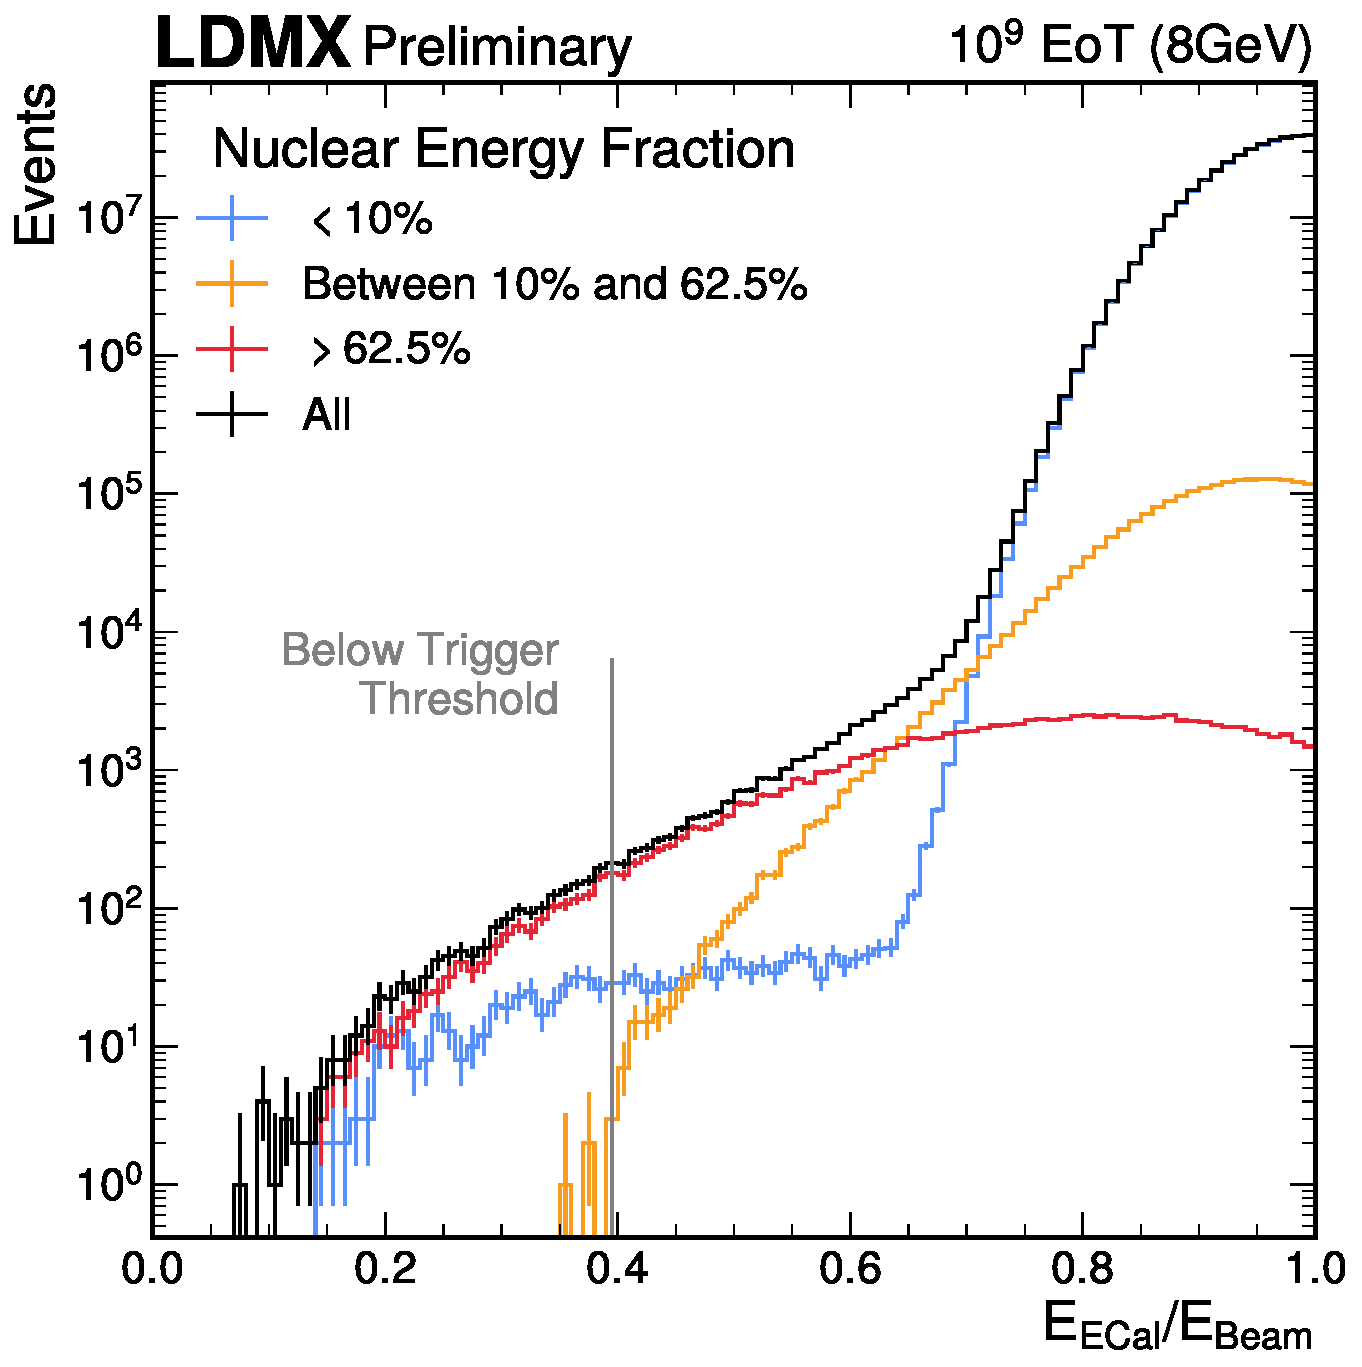
\includegraphics[width=0.9\textwidth]{../figures/ldmx/simulation/8gev-ecal-by-nuc.pdf}
        \caption{\footnotesize Reconstructed energy fraction separated by 
        energy going into nuclear processes.}
      \end{figure}
    \end{column}
    \begin{column}{0.55\textwidth}
      \begin{block}{Simulation Requirement}
        Electron reaches ECal with $> 87.5\%$ of the original beam energy.
      \end{block}

      Standard processes mimicking our signal are similar to thin-target analysis
      \begin{itemize}
        \item ``Nuclear'' processes (electrons and photons interacting with nuclei to produce hadrons)
        \item Muon pair production (via high-energy photon)
      \end{itemize}
    \end{column}
  \end{columns}
\end{frame}

\note[itemize]{
\item The standard processes we need to identify are familiar culprits
  \begin{itemize}
    \item ``Nuclear'' processes
    \item ``Di-Muon'' production via high-energy photons
  \end{itemize}
\item Handling these background will depend on the volume of data we collect
}

\begin{frame}{Target Data Volume}
  \begin{columns}
    \begin{column}{0.45\textwidth}
      \begin{figure}
        \centering
        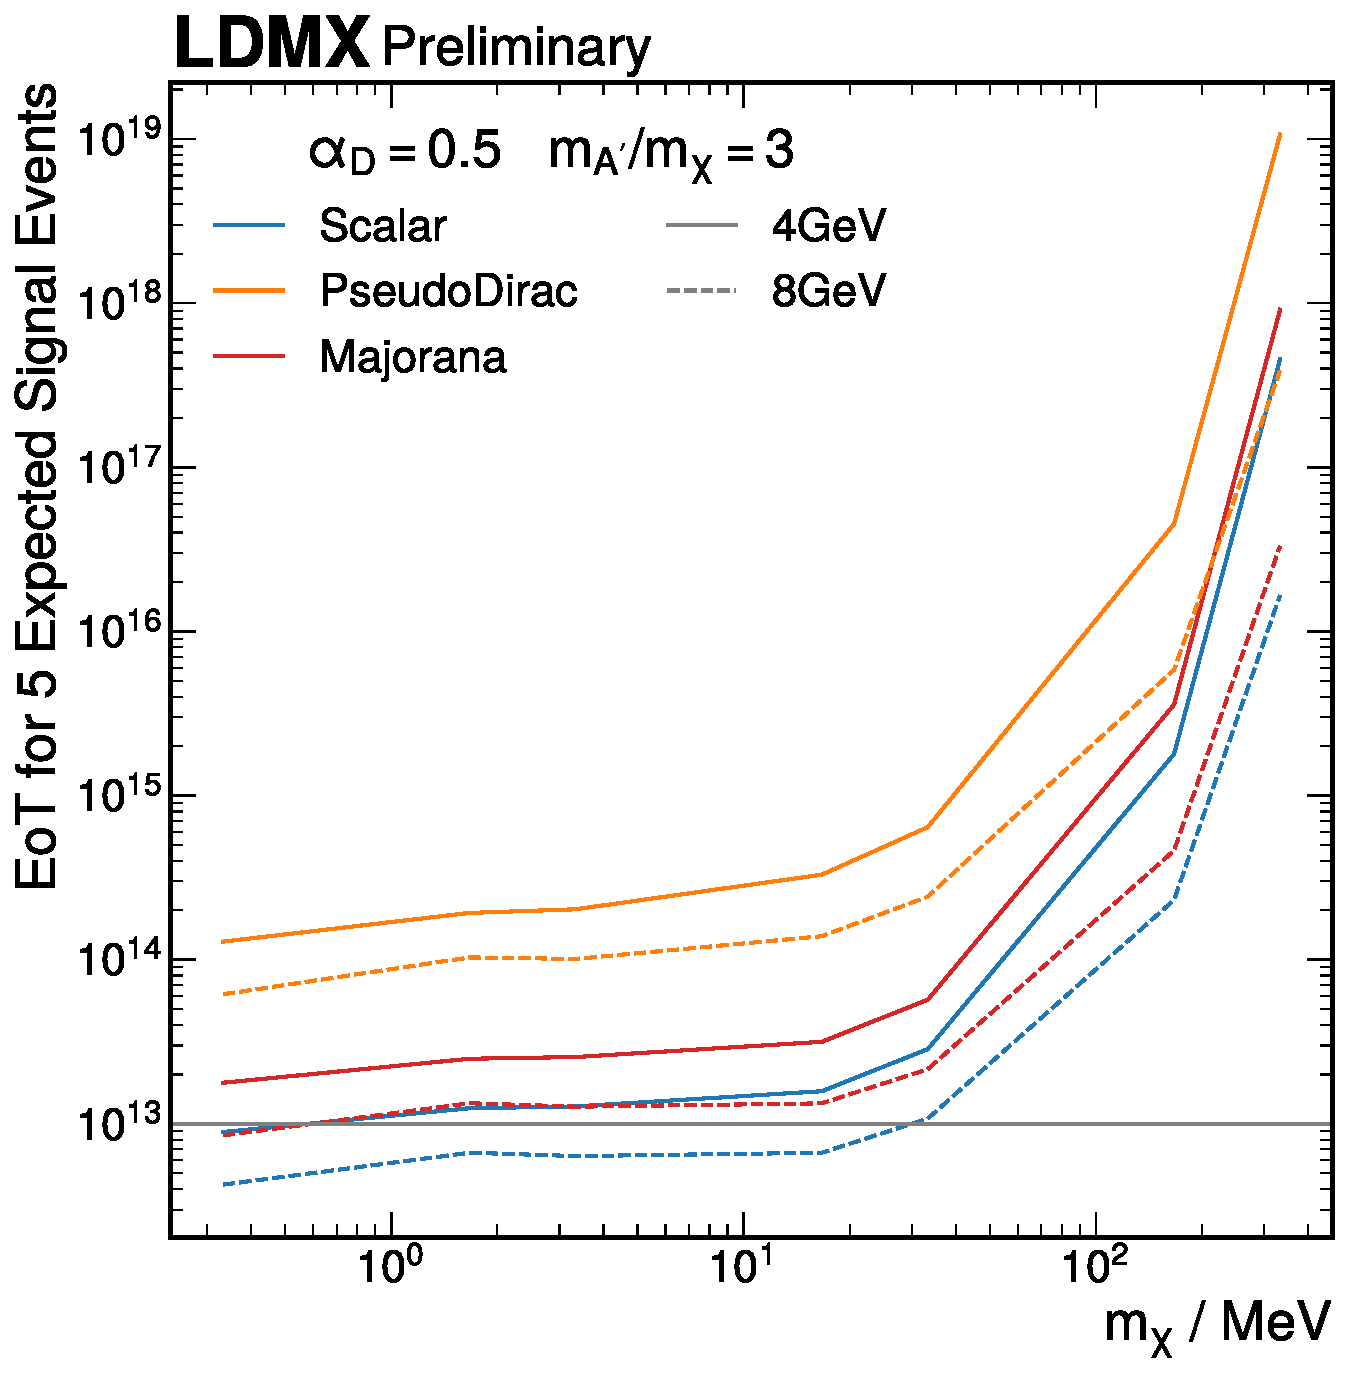
\includegraphics[width=0.9\textwidth]{figs/eot-for-n-signal.pdf}
      \end{figure}
    \end{column}
    \begin{column}{0.55\textwidth}
      \begin{itemize}
        \item Targeting $\sim 5$ expected signal events for a few possible thermal relic models
        \item Focus on \num{1e13} \ac{eot}
        \item $\sim\qty{2}{week}$ nominal beam time
      \end{itemize}

      \begin{block}{Early Running}
        Focus on first contact with real data
      \end{block}
    \end{column}
  \end{columns}
\end{frame}

\note[itemize]{
\item We choose to focuse on \num{1e13} \ac{eot} for two key reasons
  \begin{enumerate}
    \item Amounts to $\sim 5$ signal events for a few possible thermal relic models \\
      (discovery is hard for EaT -- focusing on exclusion)
    \item Only would require $\sim\qty{2}{week}$ nominal beam time
  \end{enumerate}
\item Also points out that this EaT analysis can probably be a first-contact analysis
\item Add goals of simplicity and robustness to insulate analysis from complexities of first data
}

\begin{frame}{Mid-shower Simulation Samples}
  Requirements
  \begin{itemize}
    \item Save computer time
    \item Save computer space
    \item focus on specific processes that are interesting to us \\
      (signal itself or standard processes that mimick it)
  \end{itemize}
  \vfill
  \begin{block}{Solution for Mid-Shower Samples}
    \begin{enumerate}
      \item \boldcol{UMNSunny}{Sort} simulation so higher-energy particles go first
      \item \boldcol{UMNSunny}{Bias} the process-of-interest for these high-energy particles
      \item \boldcol{UMNSunny}{Filter} out events that do not pass criteria
    \end{enumerate}
  \end{block}
\end{frame}

\note[itemize]{
\item Don't have real data yet -- need to simulate it
\item We also are focusing on specific processes (``Nuclear'' and ``Dimuon'') ocurring
  within the developing shower in the ECal
\item \textit{Requirements}
\item Developed a method to do just that -- \textit{Solution}
\item Since LDMX's beam provider LCLS-II is being upgraded separately,
  we have the potential to observe \fourgev or \eightgev beams.
\item With this technique, generated ``Nuclear'' and ``Dimuon'' samples
  statistically equivalent to \num{1e13} \ac{eot} -- combined to represent
  total ``Background''
\item \eightgev is more likely so I'll default to those figures
}

\begin{frame}{Missing Energy Signature}
  \begin{columns}
    \begin{column}{0.3\textwidth}
      \begin{enumerate}
        \item Energy measurement significantly below beam energy
        \item Nothing ``escaped'' the ECal
        \item Nothing ``funky'' happened in the ECal
      \end{enumerate}
    \end{column}
    \begin{column}{0.7\textwidth}
      \begin{tikzimage}[\textwidth]{figs/ldmx-funky-and-escape-diagram.png}
        \node[anchor=south,align=center] at (0.25,1.0) {Escaped};
        \node[anchor=south,align=center] at (0.75,1.0) {Funky};
      \end{tikzimage}
    \end{column}
  \end{columns}
\end{frame}

\note[itemize]{
\item Three key ingredients for our missing energy search
}

\begin{frame}[t]{Cuts for Missing Energy Signature}
  \begin{columns}[t]
    \begin{column}{0.32\textwidth}
      \centering
      \framesection{Low Energy Measurement}
      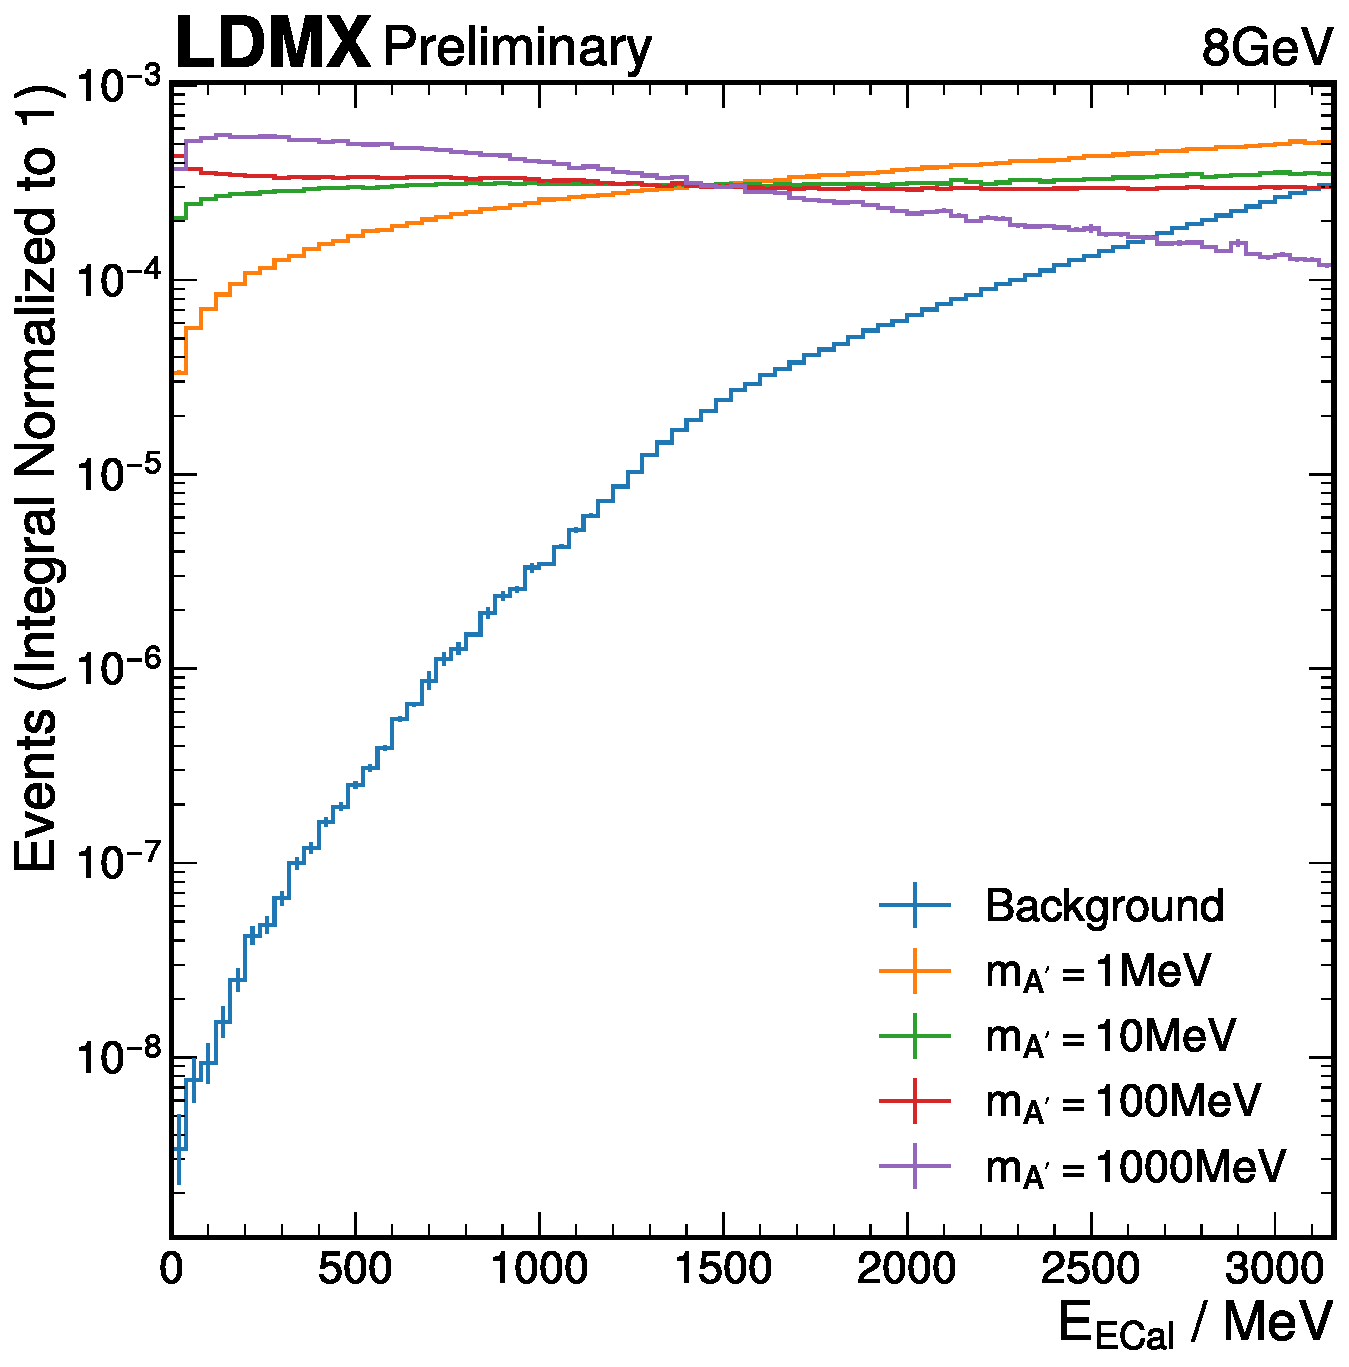
\includegraphics[width=0.9\textwidth]{../figures/ldmx/analysis/energy-after-trigger-8gev.pdf}
      {
        \footnotesize
        \begin{itemize}
          \item Use ME trigger same as nominal analysis
          \item Require lower energy on sum over all layers
        \end{itemize}
      }
    \end{column}
    \begin{column}{0.32\textwidth}
      \centering
      \framesection{Nothing Escapes}
      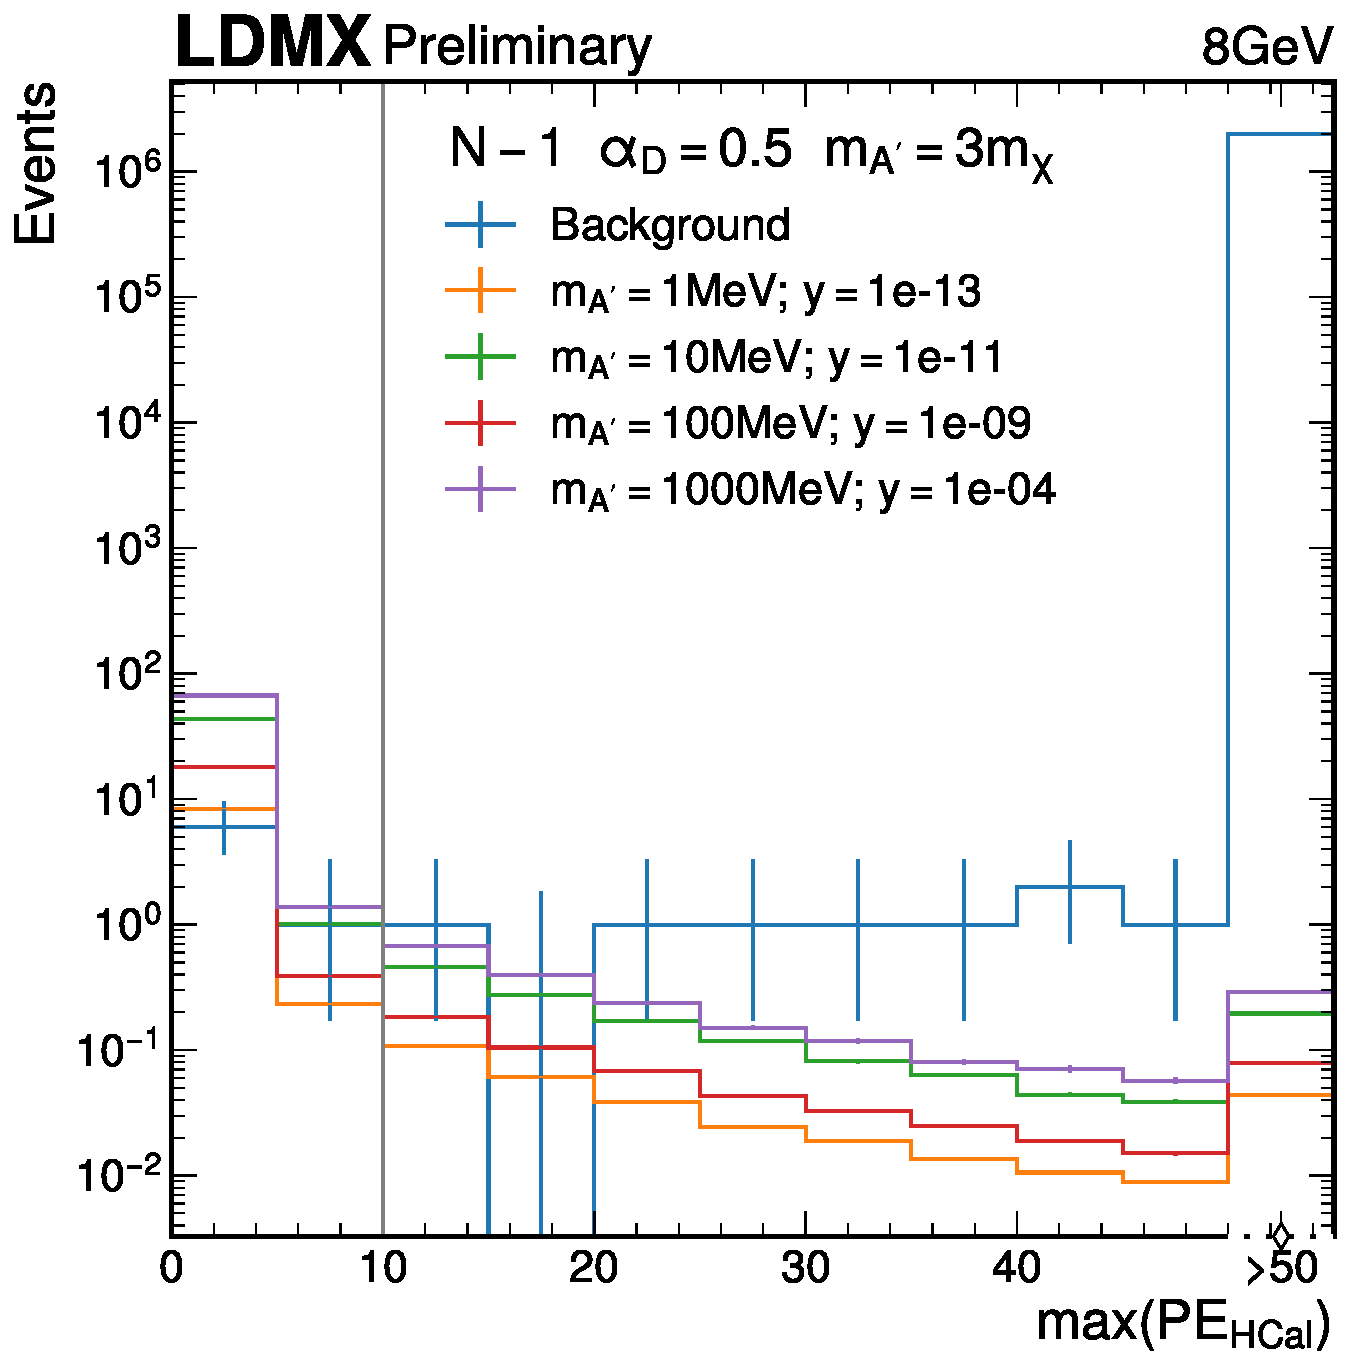
\includegraphics[width=0.9\textwidth]{../figures/ldmx/analysis/nm1-hcal-max-pe-8gev-1e13norm.pdf}
      {
        \footnotesize
        No bar within the HCal with a total signal $> \qty{10}{PE}$
      }
    \end{column}
    \begin{column}{0.32\textwidth}
      \centering
      \framesection{Nothing Funky}
      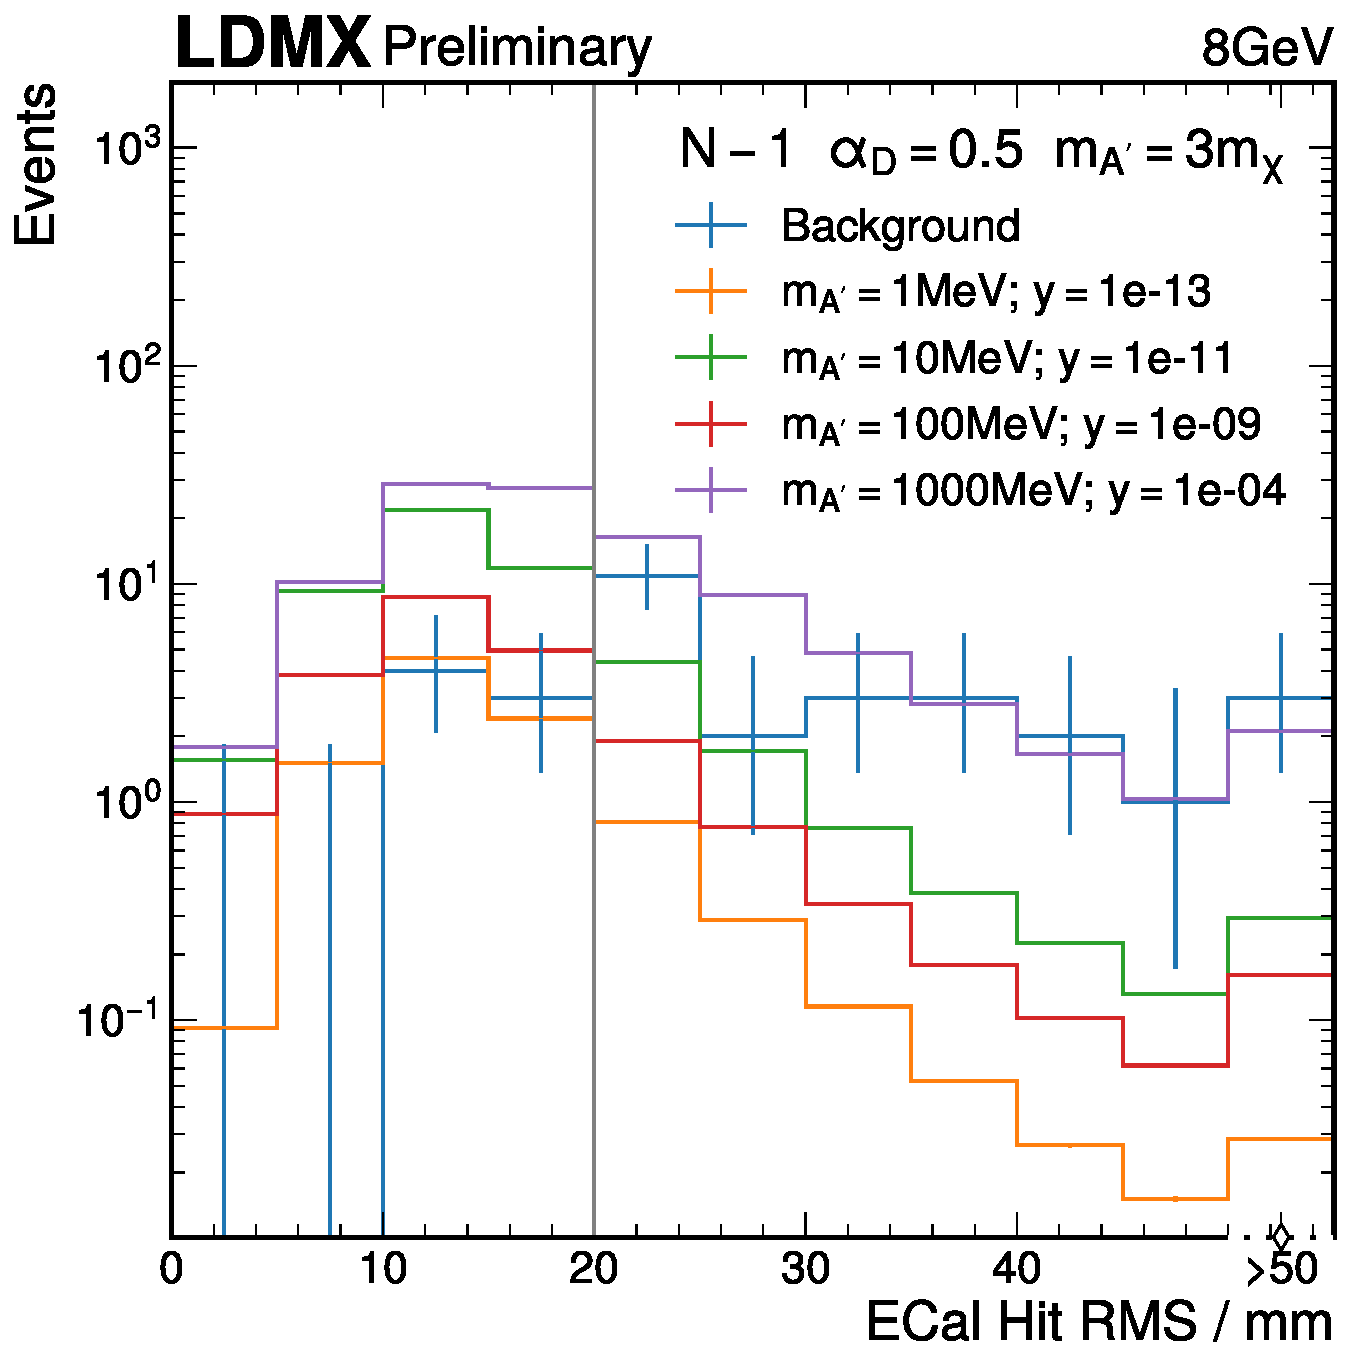
\includegraphics[width=0.9\textwidth]{../figures/ldmx/analysis/nm1-ecal-rms-8gev-1e13norm.pdf}
      {
        \footnotesize
        Energy-weighted transverse RMS of hits with amplitude $\geq 0.5E_\mathrm{MIP}$
        to be $<\qty{20}{\mm}$
      }
    \end{column}
  \end{columns}
\end{frame}

\note[itemize]{
\item Accomplish this signature using three specific variables
\item Energy sum
  \begin{itemize}
    \item After using the same trigger as the thin target MM analysis
    \item Sum over all layers and require the measurement to be \qty{400}{\MeV} less
      than the threshold used for the trigger
    \item Helps avoid contamination from miscalibrations in early running
  \end{itemize}
\item \textit{Explanatory Comma} N-1 plots show the cut variable in question after
  all other selections have been applied. Evidence that the cut is being helpful.
\item Quiet HCal
  \begin{itemize}
    \item Typical signals from muons are $\sim\qty{80}{PE}$ and other particles have higher typical signals
    \item Require no bar within HCal to register signal higher than \qty{10}{PE}
  \end{itemize}
\item Thin Shower
  \begin{itemize}
    \item Indirectly remove ``funky'' interactions by requiring hits to be close to each other
    \item Avoid hits below half a MIP 
  \end{itemize}
}

\begin{frame}{Summary of Cutflow}
  \begin{table}
    \begin{tabular}{|r|c||c|c|c|c|}
    \hline
    \multirow{2}{*}{Analysis Stage for \fourgev Beam} & 
      Background & 
      \multicolumn{4}{c|}{Signal Efficiency (\%)} 
      \\ \cline{3-6} 
    & Event Yield & $1$~MeV & $10$~MeV & $100$~MeV & $1$~GeV \\ \hline
    \ecal Trigger ($E_{20} < 1.5$~GeV) &
      \num{4.60e+07} & 58 & 67 & 71 & 83 \\
    \ecal Energy ($E_{\mathrm{\ecal}} < 1.1$~GeV) & 
      \num{1.95e+06} & 35 & 48 & 53 & 72 \\
    $\max(\text{PE}_{\text{\hcal}}) < 10$ &
      \num{1.15e+03} & 34 & 47 & 52 & 69 \\
    ECal Hit RMS $< 20\;\mathrm{mm}$ &
      126 & 28 & 37 & 41 & 33 \\
    \hline
    \hline
    \multirow{2}{*}{Analysis Stage for \eightgev Beam} & 
      Background & 
      \multicolumn{4}{c|}{Signal Efficiency (\%)} 
      \\ \cline{3-6} 
    & Event Yield & $1$~MeV & $10$~MeV & $100$~MeV & $1$~GeV \\ \hline
    \ecal Trigger ($E_{20} < 3.16$~GeV) &
      \num{6.10e+07} & 66 & 74 & 79 & 89 \\
    \ecal Energy ($E_{\text{\ecal}} < 2.76$~GeV) &
      \num{6.88e+06} & 52 & 63 & 69 & 84 \\
    $\max(\text{PE}_{\text{\hcal}}) < 10$ &
      31.8 & 50 & 61 & 67 & 81 \\
    ECal Hit RMS $< 20\;\mathrm{mm}$ &
      7 & 43 & 52 & 56 & 52
    \\ \hline
\end{tabular}

    \caption{Cutflow for this analysis.
    Background event yields are estimates for $10^{13}$ EoT.}
  \end{table}
  \vfill
\end{frame}


\note[itemize]{
\item After these simple, physically-defined selections -- background is reduced by 5 or 7
  orders of magnitude while maintaining $\sim\qty{50}{\%}$ signal efficiency
\item Still some background left, how to handle it?
}

\begin{frame}{Multi-Channel Analysis}
  \begin{block}{}
    Search within adjacent ``channels'' or ``bins'' using different shapes to our advantage
  \end{block}
  \vfill
  \begin{columns}
    \begin{column}{0.35\textwidth}
      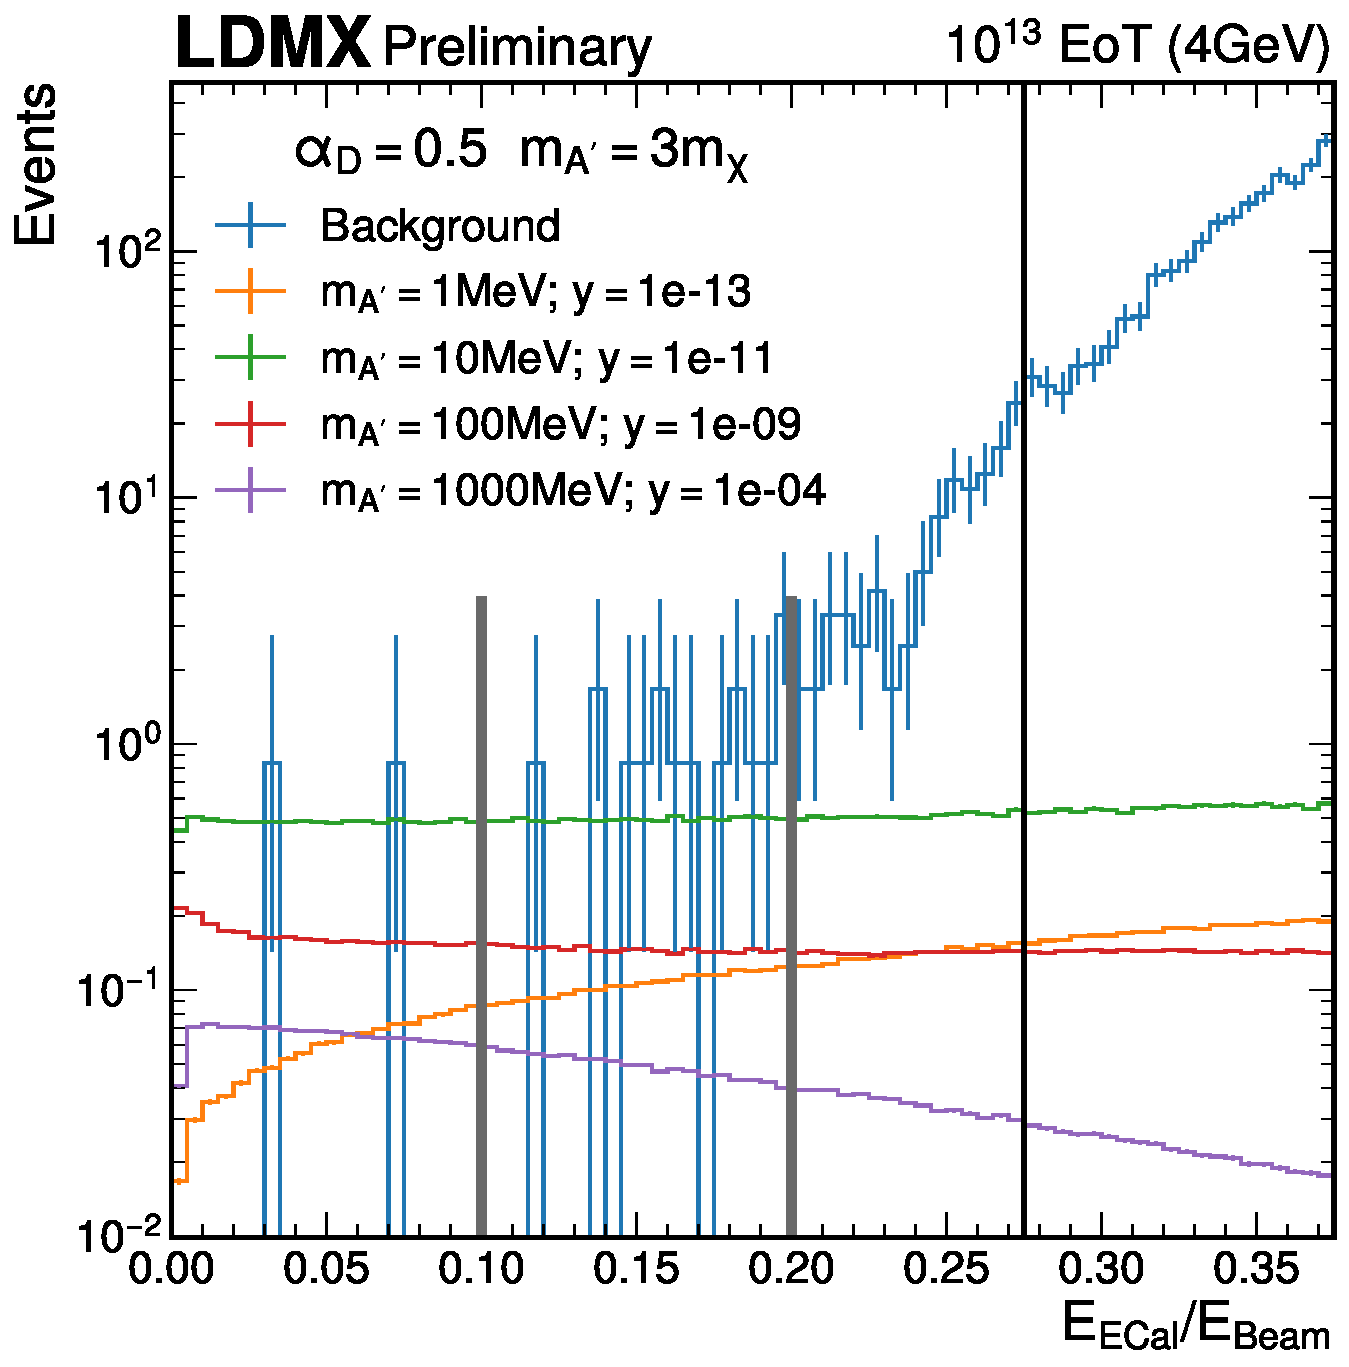
\includegraphics[width=\textwidth]{%
        ../figures/ldmx/analysis/final-selection-with-ana-bin-edges-4gev.pdf}
    \end{column}
    \begin{column}{0.35\textwidth}
      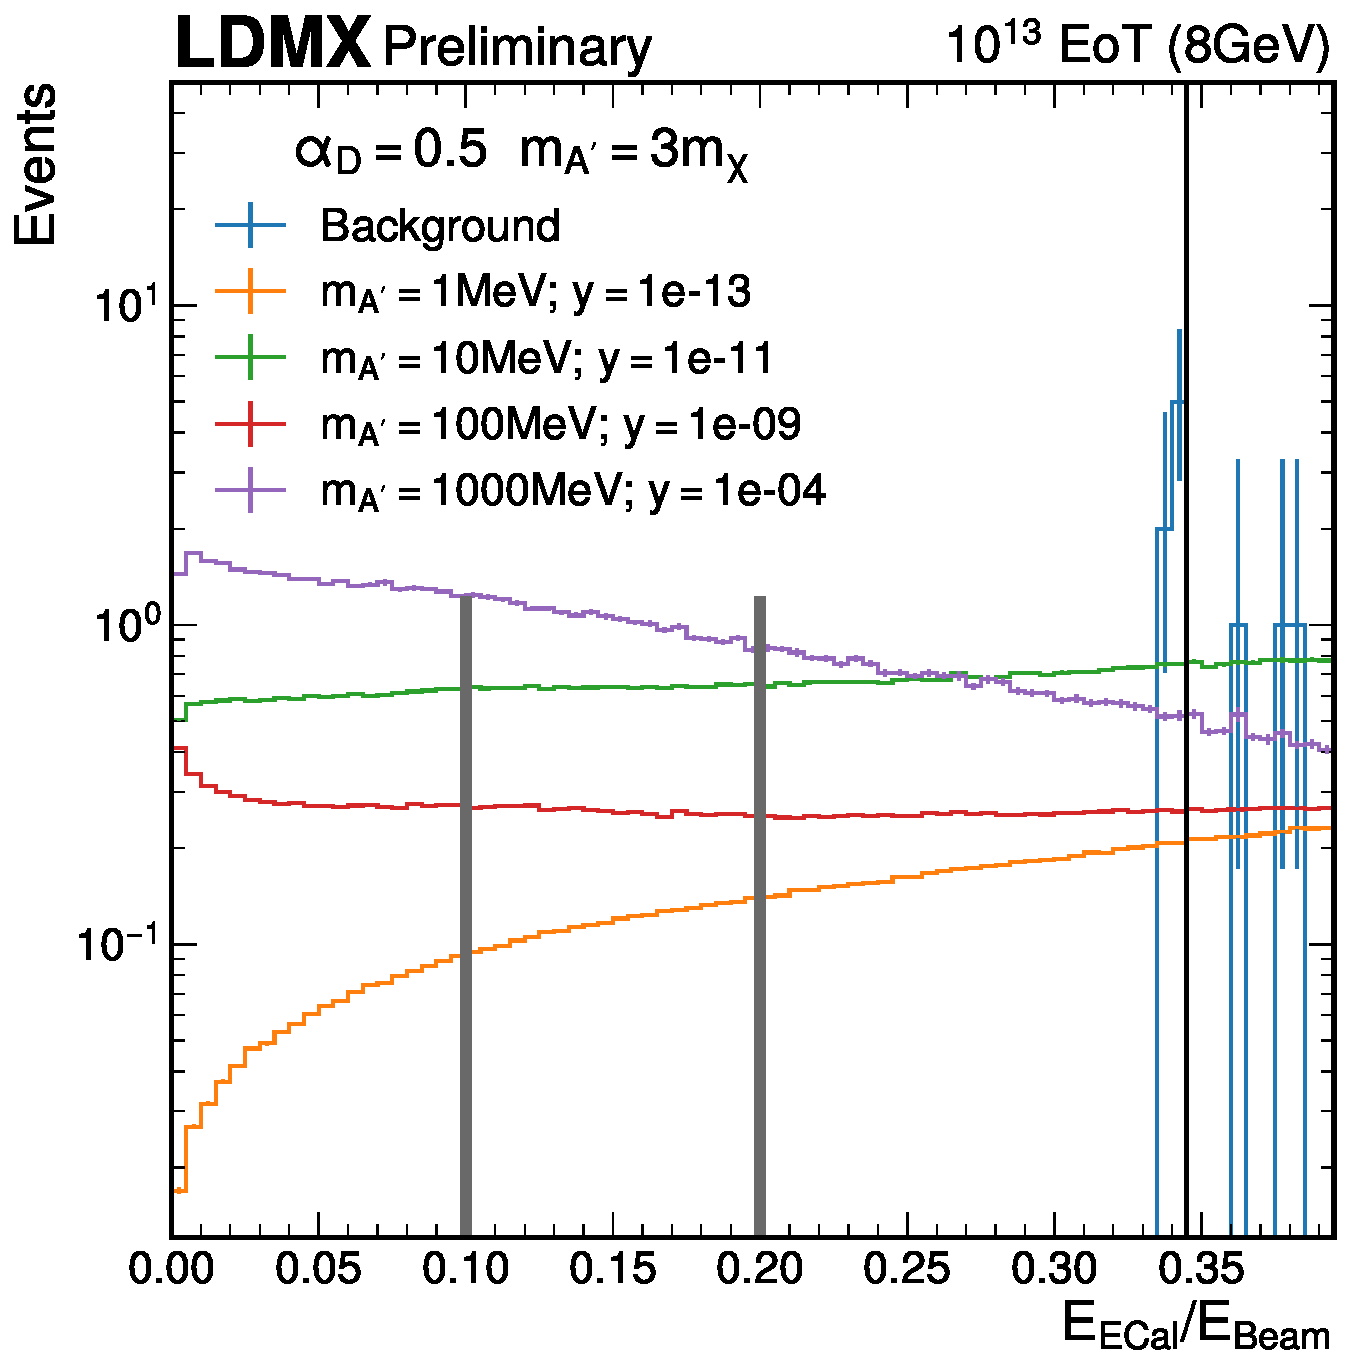
\includegraphics[width=\textwidth]{%
        ../figures/ldmx/analysis/final-selection-with-ana-bin-edges-8gev.pdf}
    \end{column}
    \begin{column}{0.3\textwidth}
      \footnotesize
      \begin{enumerate}
        \item Fit background with simple exponential function
        \item Predict background yield in three channels
        \item Separate signal efficiency into three channels
        \item Include systematic uncertainties for ECal miscalibration
          and HCal PE variation
        \item \textsc{Combine} estimates 95\% CL upper limit on signal
          production yield
      \end{enumerate}
    \end{column}
  \end{columns}
\end{frame}

\note[itemize]{
\item Can still use different shapes between signal and background to our advantage
\item Cut up final energy distribution into three bins (gray lines) with an adjacent
  control region above analysis energy threshold (black line) up to trigger threshold
  (right edge)
\item Signal is roughly evenly distributed across three bins
\item Background is sharply falling
\item Fit with control region to help constrain shape and statistical uncertainties
\item Include systematic uncertainties for ECal miscalibration and HCal PE variation
\item Use \textsc{Combine} statistical tool to estimate 95\% CL median expected limit
  on signal production yield
}

\begin{frame}{Sensitivity in Early Running}
  \begin{columns}
    \begin{column}{0.45\textwidth}
      \begin{figure}
        \centering
        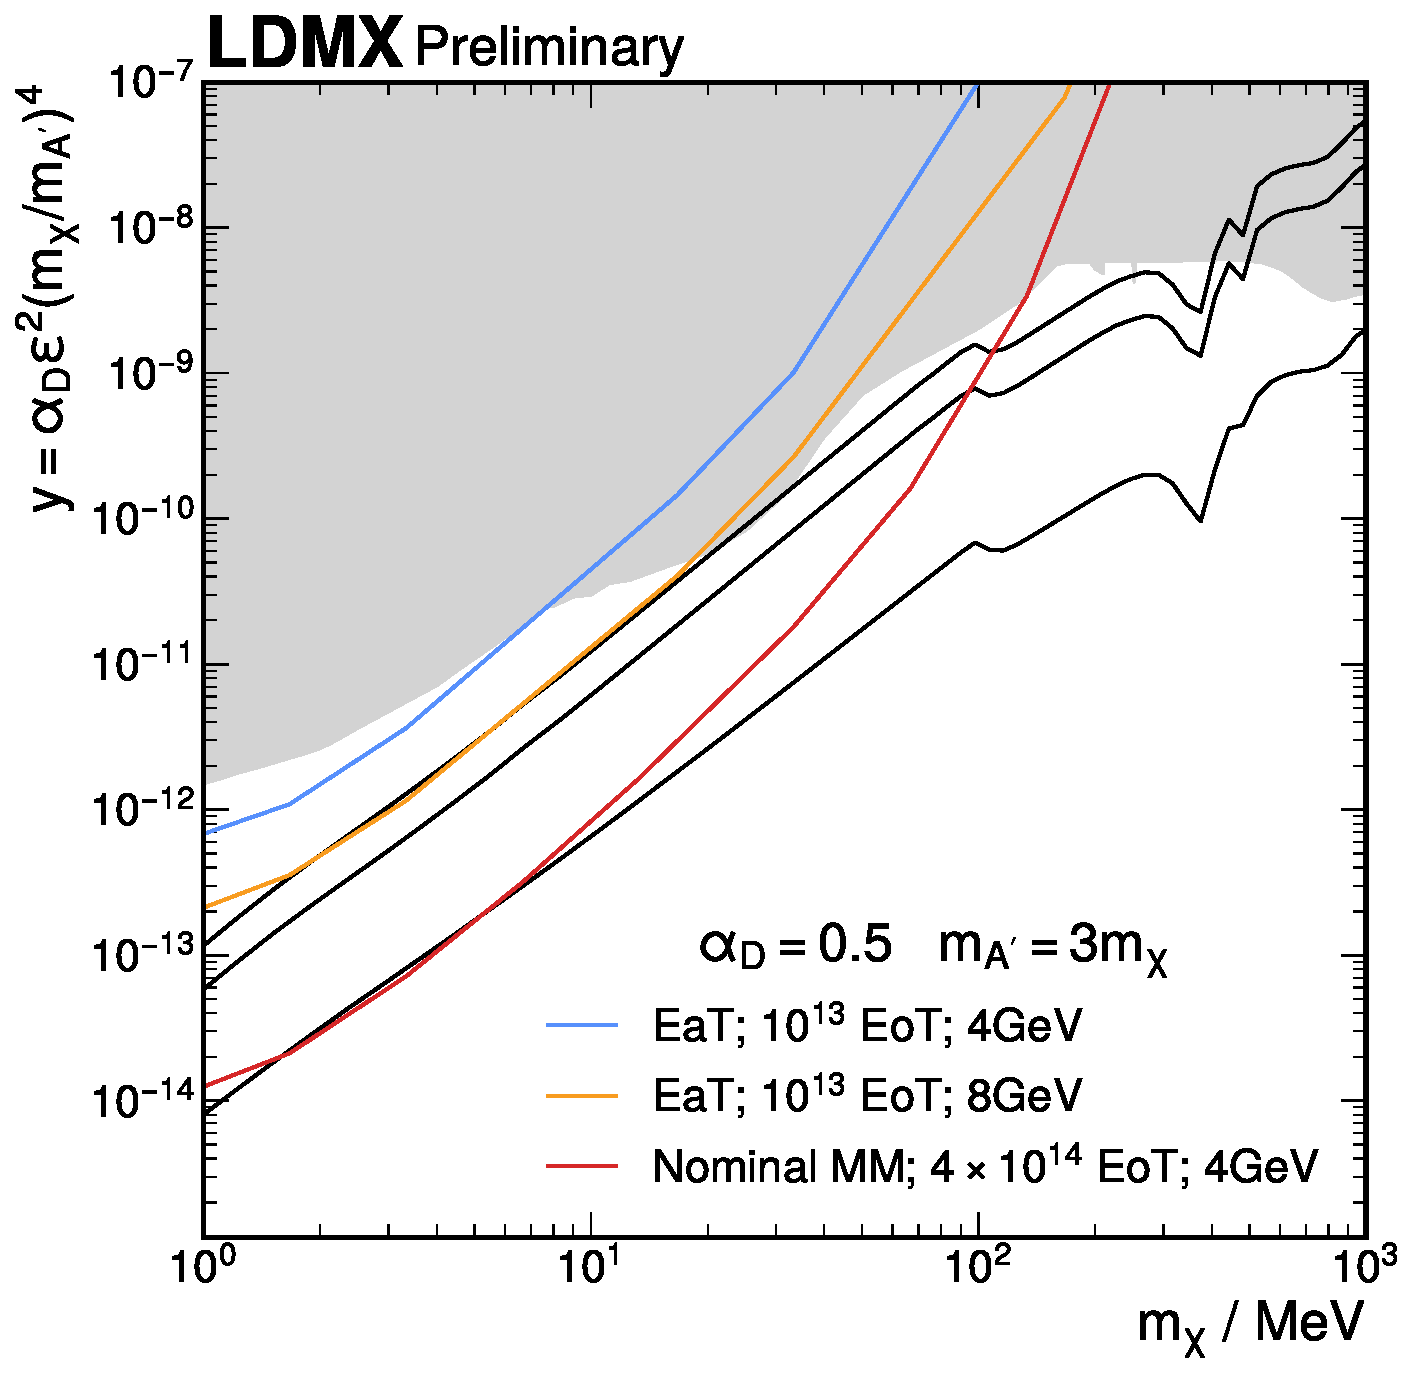
\includegraphics[width=\textwidth]{../figures/ldmx/analysis/reach.pdf}
      \end{figure}
    \end{column}
    \begin{column}{0.55\textwidth}
      \begin{itemize}
        \item For easier comparison, scale upper limit on production yield
          to lower limit on effective interaction strength $y$ using
          estimate of signal production rate
      \end{itemize}
      \vfill 
      \begin{block}{New Territory}
        Able to explore new territory of possible DM while
        learning more about our detector and setting up for
        more data enabling the full nominal analysis.
      \end{block}
    \end{column}
  \end{columns}
\end{frame}

\note[itemize]{
\item Gray is already excluded territory from experiments like NA64, BaBar, and COHERENT
\item Black lines are specific thermal relic theory expectations (From the top: Scalar, Majorana, Pseudo-Dirac)
\item Blue (Orange) is expected limit for this \fourgev (\eightgev) analysis
\item Red is nominal (missing momentum) analysis with 40x more data at \fourgev
}

\ssection{Drell-Yan Estimation}

\note[itemize]{
\item Heavy Photon Search experiment
\item HPS takes a different approach towards searching for dark brem
\item Instead of looking for extra events with missing energy/momentum,
  we look for extra events with a specific reconstructed quantities
}

\subsection{Jet $p_{T}$ Reweighting}
\begin{frame}{Visible Signature}
  \begin{columns}
    \begin{column}{0.5\textwidth}
      \begin{figure}
        \begin{tikzpicture}
          \begin{feynman}
            \vertex (beamorigin) {$e^{-}$};
            \vertex [right=of beamorigin] (beamspacer) {};
            \vertex [right=of beamspacer, circle, fill] (target) {};
            \vertex [above right= of target] (recoilspacer) {};
            \vertex [above right= of recoilspacer] (recoil) {$e^{-}$};
            \vertex [below right= of target] (propagate);
            \vertex [below right= of propagate, circle, fill] (decay) {};
            \vertex [above right= of decay] (produced) {$e^{-}$};
            \vertex [below right= of decay] (positron) {$e^{+}$};
            \diagram*[large] {
              (beamorigin) -- [fermion] (target) -- [fermion] (recoil),
              (positron) -- [fermion] (decay) -- [fermion] (produced),
              (target) -- [scalar, edge label={\boldcol{UMNMaroon}{?}}] (decay)
            };
          \end{feynman}
        \end{tikzpicture}
      \end{figure}
    \end{column}
    \begin{column}{0.5\textwidth}
      \boldcol{UMNMaroon}{Some particle} is created and then eventually
      decays back to particles we can observe.

      \begin{block}{Displaced}
        Observe produced particles ``far'' from target location due
        to lifetime of \boldcol{UMNMaroon}{?}
      \end{block}

      \begin{block}{Resonant}
        Produced particles reconstruct the mass of \boldcol{UMNMaroon}{?}
      \end{block}
    \end{column}
  \end{columns}
\end{frame}

\note[itemize]{
\item If light thermal-relic DM exists, then it interacts with SM particles somehow
\item After it is produced from dark brem, it could similarly go back into SM particles we can then observe
\item Particle question mark gets created and decays somehow but we can observe the electrons and positron
  interacting with it
\item This signature of new physics is what HPS was built for
\item Focused on electron-positron pairs that are displaced and reconstruct the mass of a previously unknown particle
\item Benefits
  \begin{itemize}
    \item Physical quantities come with any DM observation
    \item More specific event topology required for standard process to be considered background
    \item HPS can throw away a majority of the electrons that don't do anything interesting
  \end{itemize}
\item Downsides
  \begin{itemize}
    \item Need to ``go through'' mixing twice and thus need much higher data volume
    \item Dark sector needs to be ``more defined'' so we can predict
      how it decays back into standard particles
  \end{itemize}
}

\begin{frame}{Experiment}
  \resizebox{\textwidth}{!}{\begin{tikzpicture}
  \drawhps
\end{tikzpicture}
}
  \vfill
  \begin{columns}
    \begin{column}{0.32\textwidth}
      High rate $\sim\qty{500}{\MHz}$ of incident electrons
    \end{column}
    \begin{column}{0.32\textwidth}
      \qty{15}{mrad} opening angle to avoid detector damage
    \end{column}
    \begin{column}{0.32\textwidth}
      ECal for trigger and energy, SVT for tracks and vertices
    \end{column}
  \end{columns}
\end{frame}

\note[itemize]{
\item HPS installed at Thomas Jefferson Natl Lab
\item Took physics data in 2016, 2019, and 2021 -- scheduled for more data collection in coming years
\item ECal to quickly observe multiple candidate particles and make data collection decision
\item Silicon Vertex Tracker to reconstruct tracks and vertices
\item Many possible dark sectors yield the correct thermal relic abundance
  simpler one (dark photon returns back to ele-pos pair) has already been searched for
\item Choose one to focus on for further analysis
}

\begin{frame}{Strongly-Interacting Dark Sector}
  \begin{columns}
    \begin{column}{0.6\textwidth}
      \begin{figure}
        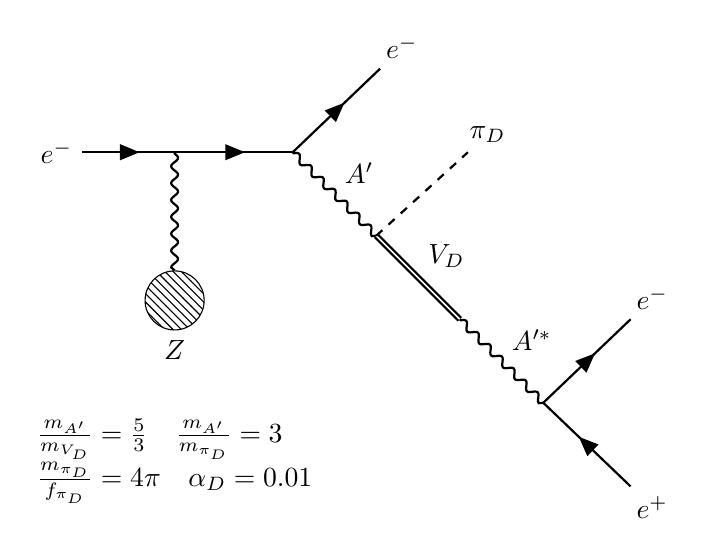
\begin{tikzpicture}
  \begin{feynman}
    \vertex (a) {$e^{-}$};
    \vertex [right= of a](d);
    \vertex [below=of d, blob,label={below:$Z$}] (e) {};
    \vertex [right= of d] (b);
    \vertex [above right= of b] (g) {$e^{-}$};
    \vertex [below right= of b] (aprime_decay);
    \vertex [below right= of aprime_decay] (rhod_decay);
    \vertex [above right= of aprime_decay] (dm) {$\pi_D$};
    \vertex [below right= of rhod_decay] (i);
    \vertex [above right= of i] (j) {$e^{-}$};
    \vertex [below right= of i] (k) {$e^{+}$};
    \diagram*[large] {
    (a) -- [fermion] (d),
    (d) -- [boson] (e),
    (d) -- [fermion] (b),
    (b) -- [fermion] (g),
    (b) -- [boson, edge label={$A'$}] (aprime_decay) -- [double, edge label={$V_D$}] (rhod_decay),
    (aprime_decay) -- [scalar] (dm),
    (rhod_decay) -- [boson, edge label={$A'^*$}] (i),
    (k) -- [fermion] (i) -- [fermion] (j),
    };
  \end{feynman}

  \node [below=of e,align=left] (param)
    {\(\frac{m_{A'}}{m_{V_D}} = \frac{5}{3}\quad\frac{m_{A'}}{m_{\pi_D}} = 3\)\\%
    \(\frac{m_{\pi_D}}{f_{\pi_D}} = 4\pi\quad\alpha_D = 0.01\)};
\end{tikzpicture}

      \end{figure}
    \end{column}
    \begin{column}{0.4\textwidth}
      {\color{UMNMaroon}
      \textbf{S}trongly-\textbf{I}nteracting \\
      \textbf{M}assive \textbf{P}articles
      }
      \begin{itemize}
        \item Dark sector contains ``dark quarks'' -- $\pi_D$ and $V_D$ are mesons like
          standard $\pi$ and $\rho$
        \good Decouples production rate from decay rate
        \bad  Extra missing energy lost to $\pi_D$ during decay chain
      \end{itemize}
      $$
        m_\mathrm{reco} = m_{V_D} \qquad
        z_\mathrm{reco} \sim e^{-z/(c\tau_{V_D})}
      $$
    \end{column}
  \end{columns}
\end{frame}

\note[itemize]{
\item HPS's 2016 dataset is relatively small meaning a simpler dark sector that has
  the dark photon decaying back to electron-positron pair itself was not reachable
\item SIMPs decouple the production and decay rate allowing real sensitivity for HPS
  within this smaller dataset
\item Observables
  \begin{itemize}
    \item[$\to$] Reconstructed mass peaking at dark vector mass
    \item[$\to$] Excess of highly-displaced vertices from decay length of dark vector
  \end{itemize}
\item HPS geometric and trigger acceptance basically requires $A'$ and $V_D$ to be
  colinear with incident electron
  \begin{itemize}
    \item Not difficult for $A'$ since it takes a vast majority of the incident electrons' energy
  \end{itemize}
}

\begin{frame}{Data Collection Trigger}
  \begin{figure}
    \centering
    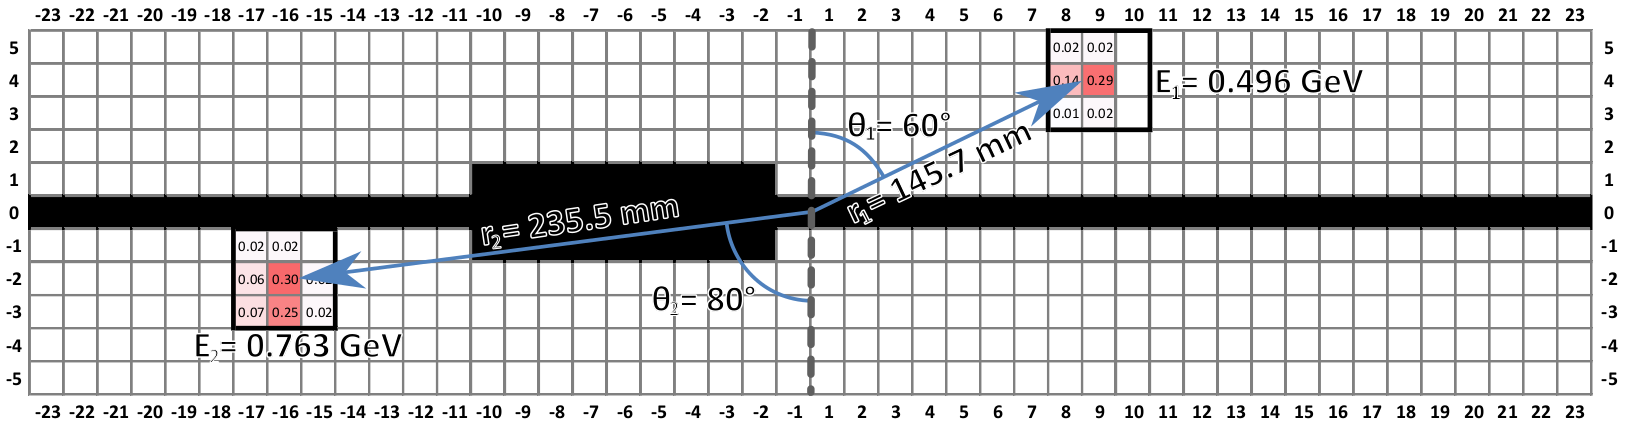
\includegraphics[width=\textwidth]{%
      ../figures/hps/experiment/skmccarty-thesis-fig-27-pair-trigger-depiction.png}
    \caption{Diagram of ECal Pair Trigger. Fig 27 from S K McCarty Thesis 2020.}
  \end{figure}
\end{frame}

\note[itemize]{
\item Credit to SK McCarty for studying and tuning these trigger parameters
\item Individual clusters have at least 2 hits and \qty{0.15}{\GeV} and at most \qty{1.40}{\GeV}
\item Pair energy sum has between \qty{0.6}{\GeV} and \qty{2}{\GeV}
\item Pair energy difference less than \qty{1.14}{\GeV}
\item Low energy cluster matching curvature from magnetic field (roughly)
\item Pair within \qty{35}{\degree} of opposite
}

\begin{frame}{Preliminary Quality Selections}
  \begin{columns}
    \begin{column}{0.35\textwidth}
      \centering
      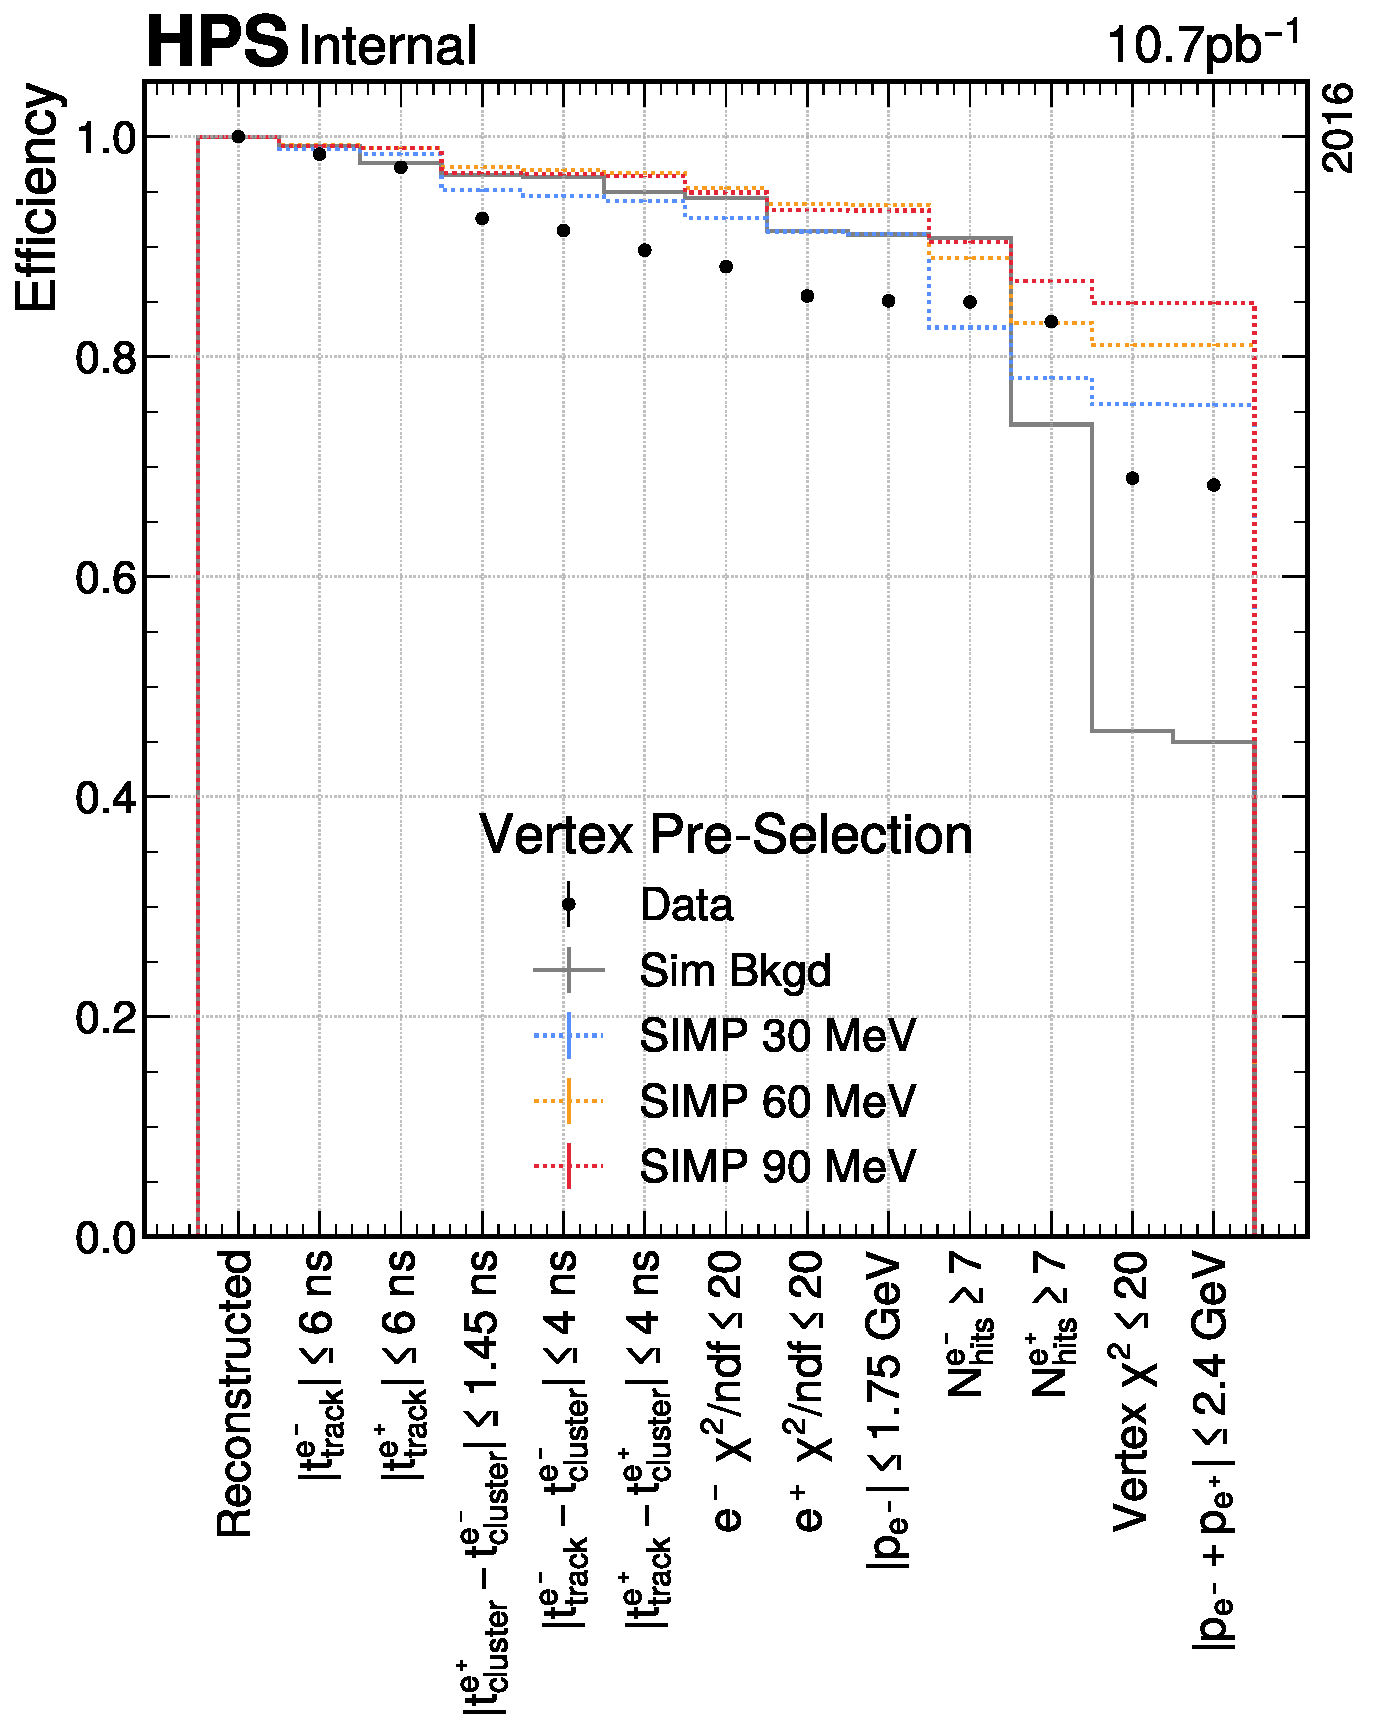
\includegraphics[width=\textwidth]{%
        ../figures/hps/dataset/vertex-pre-selection-efficiency.pdf}
    \end{column}
    \begin{column}{0.3\textwidth}
      Count number of vertices passing the
      quality selections
    \end{column}
    \begin{column}{0.35\textwidth}
      \centering
      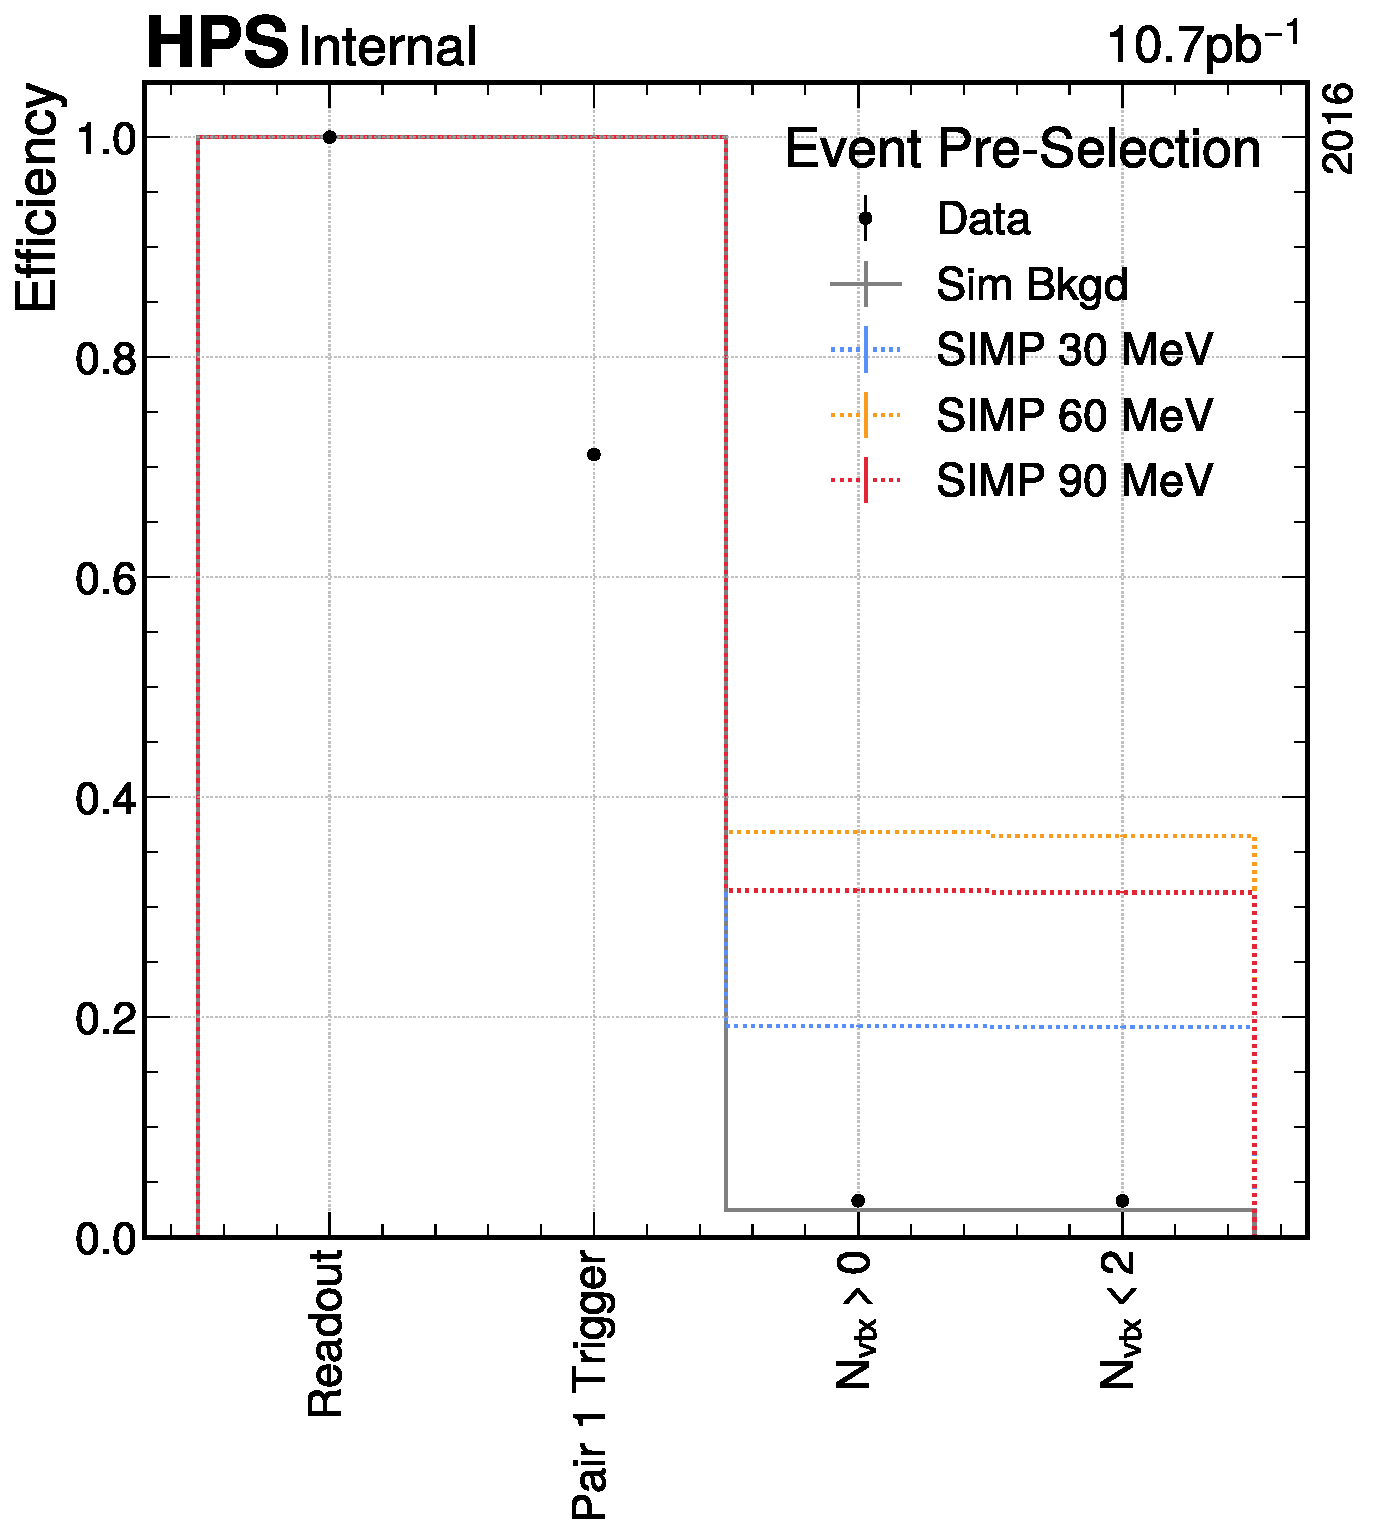
\includegraphics[width=\textwidth]{%
        ../figures/hps/dataset/event-pre-selection-efficiency.pdf}
    \end{column}
  \end{columns}
\end{frame}

\note[itemize]{
\item After this trigger selection, we apply some more selections to focus
  on higher quality vertices
\item Credit to A Spellmen for studying and tuning this pre-selection
\item Requirement that a vertex is reconstructed is biggest difficulty,
  reflects (roughly) the geometric acceptance of the detector
}

\begin{frame}{L1L1 and L1L2}
  \begin{columns}
    \begin{column}{0.3\textwidth}
      \resizebox{\textwidth}{!}{\begin{tikzpicture}
  \drawhpsfirsttwolayers
  \node at (\targetx,+2) {L1L1};
  \node at (\targetx+1,0.1) [circle,fill,inner sep=1.5pt] {};
  \draw[black,->] (\targetx+1,0.1) -- (2.5,2) node[anchor=north west] {\(e^-\)};
  \draw[black,->] (\targetx+1,0.1) -- (2.5,-1.9) node[anchor=south west] {\(e^+\)};
\end{tikzpicture}
}
      \resizebox{\textwidth}{!}{\begin{tikzpicture}
  \drawhpsfirsttwolayers
  \node at (\targetx,+2) {L1L2};
  \node at (\targetx+2.0,0.1) [circle,fill,inner sep=1.5pt] {};
  \draw[black,->] (\targetx+2.0,0.1) -- (2.5,2) node[anchor=north west] {\(e^-\)};
  \draw[black,->] (\targetx+2.0,0.1) -- (2.5,-1.8) node[anchor=south west] {\(e^+\)};
\end{tikzpicture}
}
    \end{column}
    \begin{column}{0.6\textwidth}
      Quality of reconstruction is closely tied with how many (and which)
      tracker layers are hit.
      \begin{itemize}
        \item Helpful to separate analyses into reconstruction categories
      \end{itemize}
      \vfill
      \begin{block}{Orthogonal Analyses}
        Experiment design categories (should) have no effect on observable
        physics so they are helpful cross checks for each other.
      \end{block}
    \end{column}
  \end{columns}
\end{frame}

\note[itemize]{
\item \textit{Quality -- Categories}
\item L1L1 requires all four sensors in first two layers to have hits for both tracks
\item L1L2 drops the first layer requirement for only one of the tracks
\item L1L2 vertices are more ``contaminated'' but also reach to higher displacements
}

\begin{frame}{Basic, Fixed Selection}
  \begin{itemize}
    \item \boldcol{UMNSunny}{L1L2}: In the vertex, one of the particles 
      must have a hit in both sensors in Layer 1 and Layer 2
      while the other must have a hit in both sensors in Layer 2 and Layer 3.
      \begin{itemize}
        \item The reconstruction category I am studying
      \end{itemize}
    \item \boldcol{UMNSunny}{Low Momentum Sum}:
      $\qty{1.0}{\GeV} < P_\mathrm{sum} < \qty{1.9}{\GeV}$
      \begin{itemize}
        \item Missing energy ``lost`` to $\pi_D$
      \end{itemize}
    \item \boldcol{UMNSunny}{Decay after Target}: $z > z_\mathrm{target}$
      \begin{itemize}
        \item Redundant with the \minyzero cut, but ensures decay weights
          don't unphysically diverge
      \end{itemize}
    \item \boldcol{UMNSunny}{Mass Window}: $p_m < 1.5$ (search SR),
      $1.5 < p_m < 4.5$ (search sideband)
      \begin{itemize}
        \item electron-positron pair has mass within resolution of $V_D$ test mass
      \end{itemize}
  \end{itemize}
  $$
    p_m = \frac{|m_\mathrm{reco}-m_{V_D}|}{\sigma_m}
  $$

  \begin{block}{Optimization}
    Optimize further cuts on 10\% subsample of data
  \end{block}
\end{frame}

\note[itemize]{
\item The L1L1 category, consisting of higher-quality vertices, has already
  been studied, helpfully optimizing many selections that are easily applicable
  to the L1L2 category as well
\item \textit{Selections}
\item Using sub-sample of data in order to avoid background simulation that
  is not trustworthy
}

\begin{frame}{Helpful Physics Variable}
  \begin{block}{Vertical Impact Parameter $y_0$}
    gives helpful insight into displaced nature of vertex
  \end{block}
  \begin{figure}
    \begin{subfigure}{0.32\textwidth}
      \resizebox{\textwidth}{!}{\begin{tikzpicture}
  \drawhpsfirsttwolayers
  \draw[black] (\targetx-\targethalfthick,0) -- (2.5,0);
  \node[anchor=north west,align=left,text depth=\baselineskip] at (\targetx,+3)
    {Truly\\Displaced};
  \node at (\targetx+2,0.1) [vertex] {};
  \draw[black,->] (\targetx+2.0,0.1) -- (2.5,2) node[anchor=north west] {\(e^-\)};
  \node at (\layeronex-\sensorhalfsep,\elelayeronestereoy) [hit] {};
  \node at (\layeronex+\sensorhalfsep,\elelayeroneaxialy) [hit] {};
  \node at (\layertwox-\sensorhalfsep,\elelayertwostereoy) [hit] {};
  \node at (\layertwox+\sensorhalfsep,\elelayertwoaxialy) [hit] {};
  \draw[black,->] (\targetx+2.0,0.1) -- (2.5,-1.8) node[anchor=south west] {\(e^+\)};
  \node at (\layeronex-\sensorhalfsep,\poslayeronestereoy) [miss] {};
  \node at (\layeronex+\sensorhalfsep,\poslayeroneaxialy) [miss] {};
  \node at (\layertwox-\sensorhalfsep,\poslayertwostereoy) [hit] {};
  \node at (\layertwox+\sensorhalfsep,\poslayertwoaxialy) [hit] {};
  \draw[black,dotted]
    (\targetx+2,0.1) -- (\targetx,\eleyzero)
    (\targetx+2,0.1) -- (\targetx,\posyzero);
  \draw[decoration={brace,raise=5pt},decorate]
    (\targetx,\eleyzero) -- node[left=6pt] {$y_{0}^{e^-}$} (\targetx,0);
  \draw[decoration={brace,raise=5pt},decorate]
    (\targetx,0) -- node[left=6pt] {$y_{0}^{e^+}$} (\targetx,\posyzero);
\end{tikzpicture}
}
    \end{subfigure}
    \begin{subfigure}{0.32\textwidth}
      \resizebox{\textwidth}{!}{\begin{tikzpicture}
  \drawhpsfirsttwolayers
  \draw[black] (\targetx-\targethalfthick,0) -- (2.5,0);
  \node[anchor=north west,align=left] at (\targetx,+3)
    {Fake Displaced\\$y_0^{e^-}\approx\qty{0}{\mm}$};

  \draw[black,->] (\targetx+\targethalfthick,0.0) -- (2.5,2) node[anchor=north west] {\(e^-\)};
  \node at (\layeronex-\sensorhalfsep,\fdelelayeronestereoy) [hit] {};
  \node at (\layeronex+\sensorhalfsep,\fdelelayeroneaxialy) [hit] {};
  \node at (\layertwox-\sensorhalfsep,\fdelelayertwostereoy) [hit] {};
  \node at (\layertwox+\sensorhalfsep,\fdelelayertwoaxialy) [hit] {};

  \draw[black,->] (\fdposx, \fdposy) -- (2.5,-1.8) node[anchor=south west] {\(e^+\)};
  \draw[dashed] (\layertwox,\fdposlayertwoaxialy) -- (\targetx+\targethalfthick,0.0)
    node[near start,below,sloped,font=\scriptsize] {True \(e^+\)};
  \node at (\layeronex-\sensorhalfsep,\fdbadhitstereoy) [hit] {};
  \node at (\layeronex+\sensorhalfsep,\fdbadhitaxialy) [miss] {};
  \node at (\layeronex-\sensorhalfsep,\fdtruhitstereoy) [miss] {};
  \node at (\layeronex+\sensorhalfsep,\fdtruhitaxialy) [miss] {};
  \node at (\layertwox-\sensorhalfsep,\fdposlayertwostereoy) [hit] {};
  \node at (\layertwox+\sensorhalfsep,\fdposlayertwoaxialy) [hit] {};

  \node at (\fdposx,\fdposy) [vertex] {};

  \draw[black,dotted] (\fdposx,\fdposy) -- (\targetx,\fdposyzero);

  \draw[decoration={brace,raise=5pt},decorate]
    (\targetx,0) -- node[left=6pt] {$y_{0}^{e^+}$} (\targetx,\fdposyzero);

%  \node[vertex,label=right:{Vertex}] (vtxlabel) at (\targetx,-2.0) {};
%  \node[hit,label=right:{Hit},below=5.0pt of vtxlabel] (hitlabel) {};
%  \node[miss,label=right:{Missed},below=5.0pt of hitlabel] {};

%  \node[vertex,label=right:{Vertex}] (vtxlabel) at (\targetx,+3.0) {};
%  \node[hit,label=right:{Hit}] at (\targetx+1.8,+3.0) {};
%  \node[miss,label=right:{Missed}] at (\targetx+3.0,+3.0) {};
\end{tikzpicture}
}
    \end{subfigure}
    \begin{subfigure}{0.32\textwidth}
      \resizebox{\textwidth}{!}{\begin{tikzpicture}
  \drawhpsfirsttwolayers
  \draw[black] (\targetx-\targethalfthick,0) -- (2.5,0);

  \node[anchor=north west,align=left] at (\targetx,+3)
    {Not Displaced\\$y_0^{e^-}\approx\qty{0}{\mm}$\\$y_0^{e^+}\approx\qty{0}{\mm}$};
  \draw[black,->] (\targetx+\targethalfthick,0.0) -- (2.5,2) node[anchor=north west] {\(e^-\)};
  \node at (\layeronex - \sensorhalfsep, \ndelelayeronestereoy) [hit] {};
  \node at (\layeronex + \sensorhalfsep, \ndelelayeroneaxialy) [hit] {};
  \node at (\layertwox - \sensorhalfsep, \ndelelayertwostereoy) [hit] {};
  \node at (\layertwox + \sensorhalfsep, \ndelelayertwoaxialy) [hit] {};
  
  \draw[black,->] (\targetx+\targethalfthick,0.0) -- (2.5,-1.8) node[anchor=south west] {\(e^+\)};
  \node at (\layeronex - \sensorhalfsep, \ndposlayeronestereoy) [miss] {};
  \node at (\layeronex + \sensorhalfsep, \ndposlayeroneaxialy) [hit] {};
  \node at (\layertwox - \sensorhalfsep, \ndposlayertwostereoy) [hit] {};
  \node at (\layertwox + \sensorhalfsep, \ndposlayertwoaxialy) [hit] {};

  \node at (\targetx+\targethalfthick,0.0) [vertex] {};
\end{tikzpicture}
}
    \end{subfigure}
  \end{figure}
  $$
    y_{0,\min} = \min(|y_0^{e^+}|,|y_0^{e^-}|)
  $$
\end{frame}

\note[itemize]{
\item Exploring data found that the vertical impact parameter $y_0$ is helpful
\item Both tracks high for truly displaced
\item Either or both near zero for fake and not displaced
\item Use variable ``minimum y zero'' to make this distinction
}

\begin{frame}{Helpful Physics Variables}
  \begin{columns}
    \begin{column}{0.3\textwidth}
      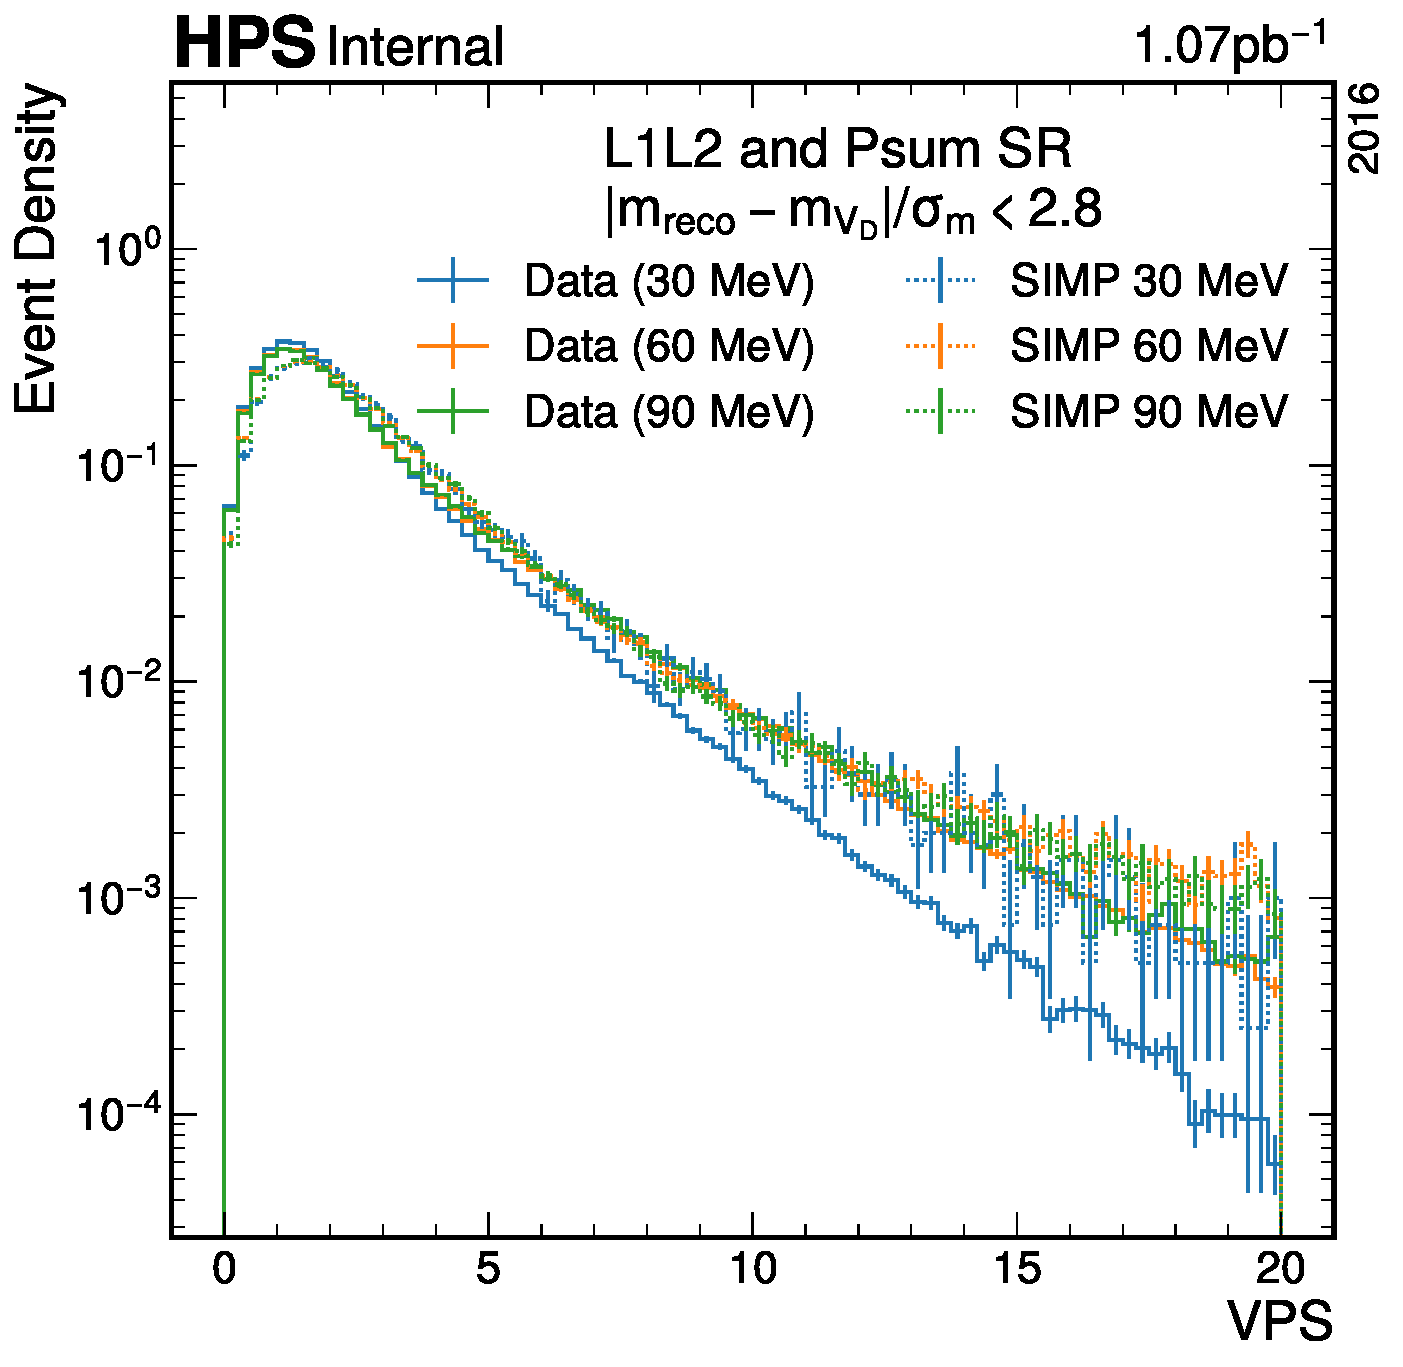
\includegraphics[width=\textwidth]{%
        ../figures/hps/analysis/vtx_proj_sig-distribution.pdf}
      \ac{vps} measures how close vertex
      is to originating from beam spot
    \end{column}
    \begin{column}{0.3\textwidth}
      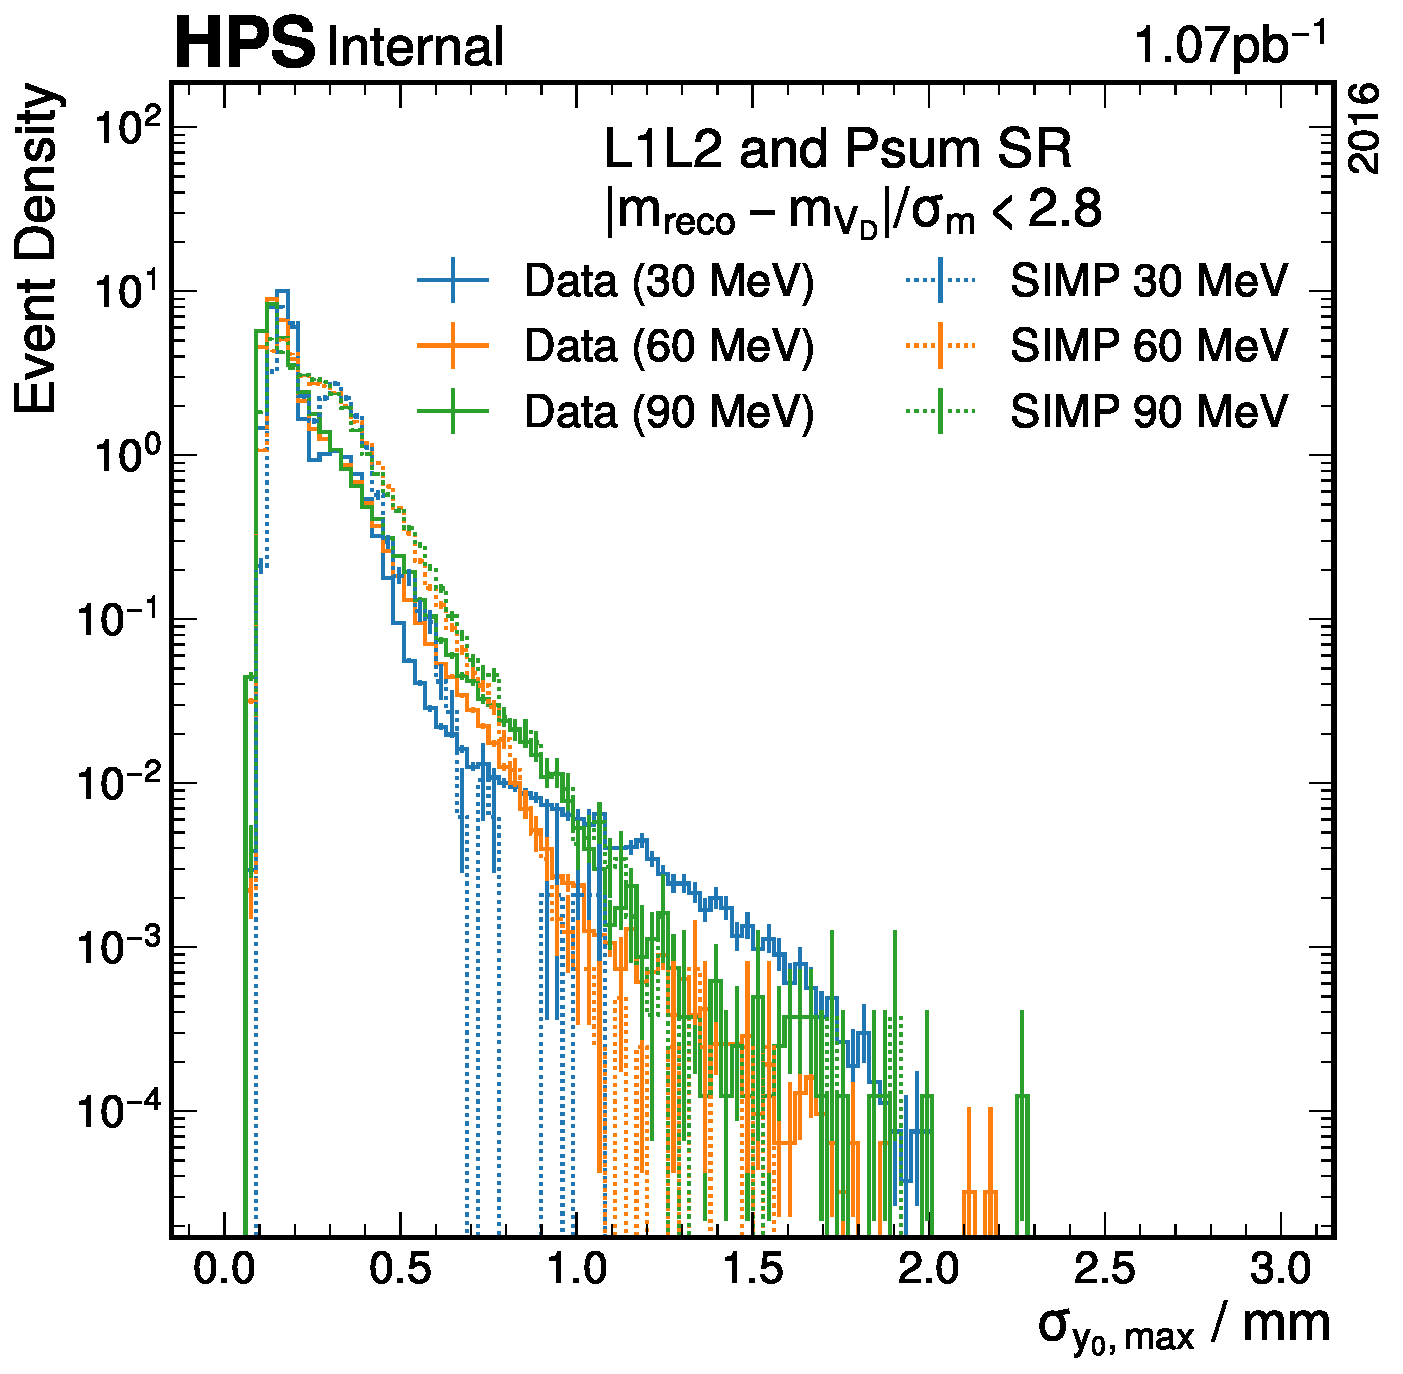
\includegraphics[width=\textwidth]{%
        ../figures/hps/analysis/max_y0_err-distribution.pdf}
      \maxyzeroerr requires high precision
      of vertical impact parameter
    \end{column}
    \begin{column}{0.3\textwidth}
      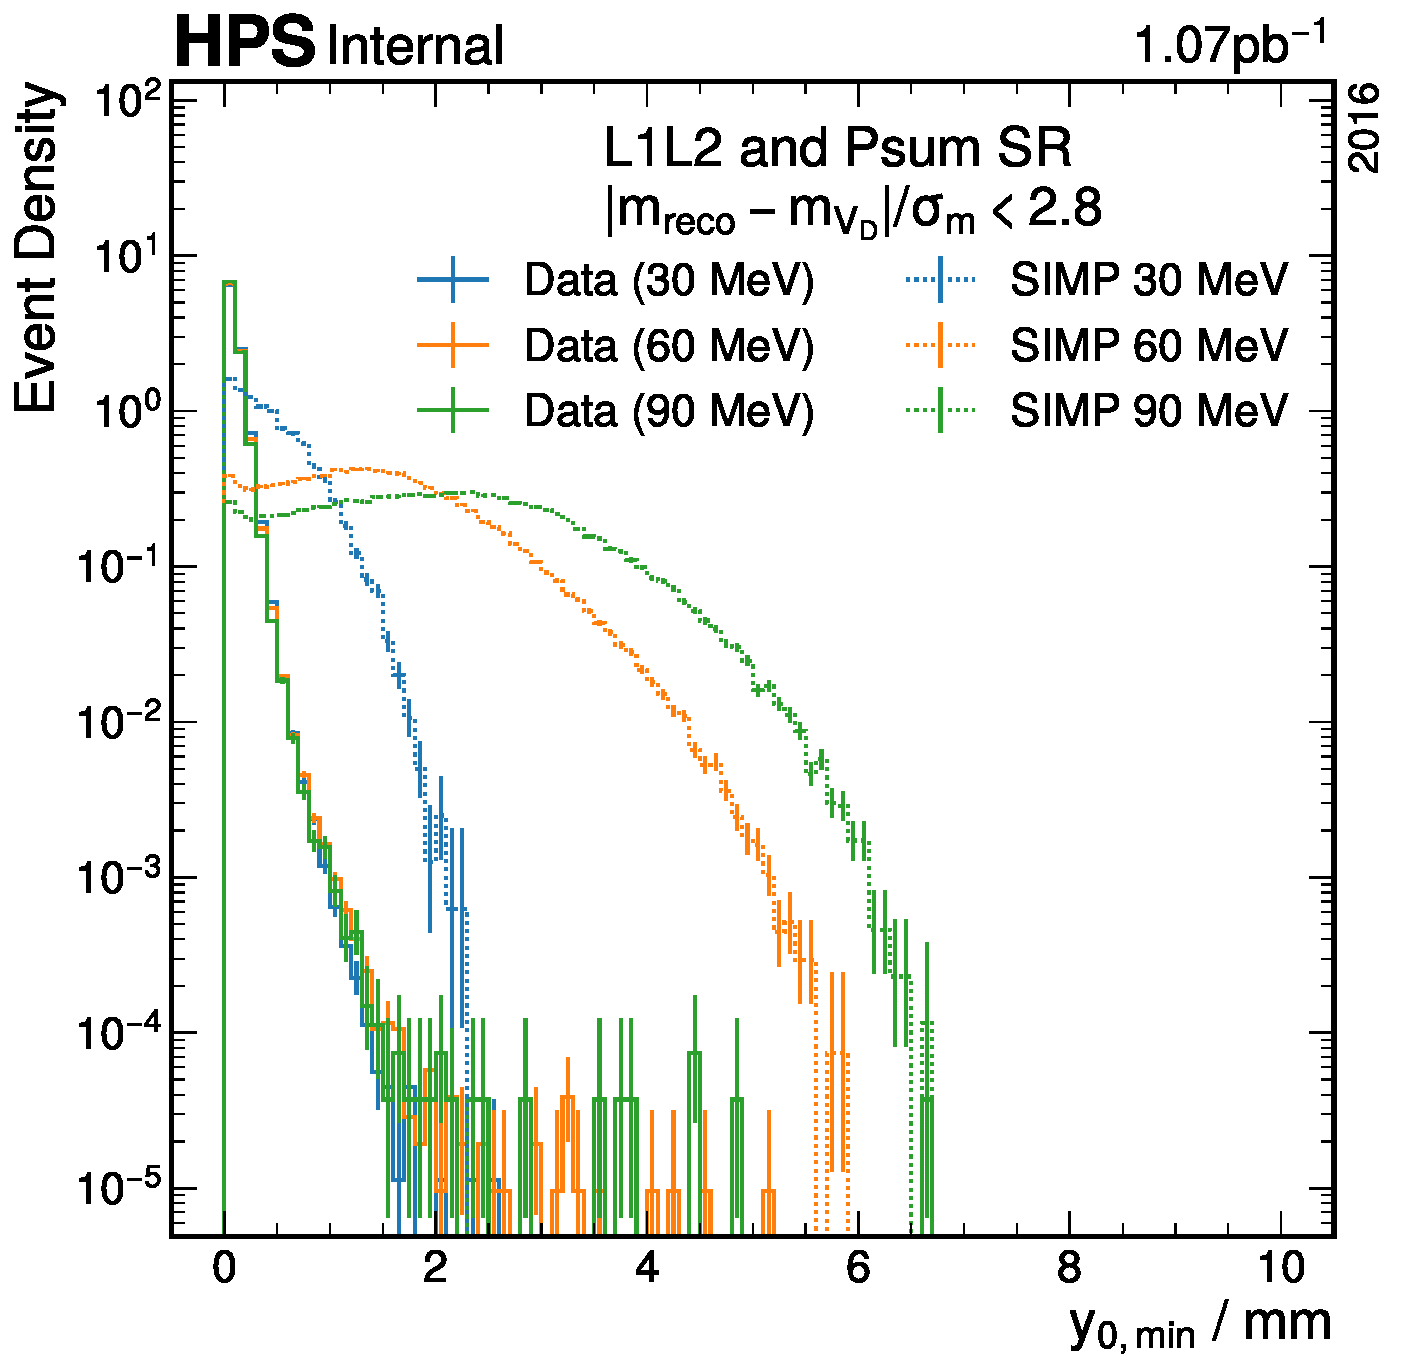
\includegraphics[width=\textwidth]{%
        ../figures/hps/analysis/min_y0-distribution.pdf}
      \minyzero separates signal and background
      with better resolution compared to others
      (like $z$ for example)
    \end{column}
  \end{columns}
\end{frame}

\note[itemize]{
\item Two additional quality requirements help \minyzero
\item \ac{vps} helps ensure vertex originates from beamspot
\item Limiting error on $y_0$
}

\begin{frame}{Optimization Procedure}
  \begin{columns}
    \begin{column}{0.3\textwidth}
      {Keep relative signal efficiency high ($> \qty{80}{\%}$)
      while trimming data tail of \minyzero distribution.}
      
      \vfill

      {
      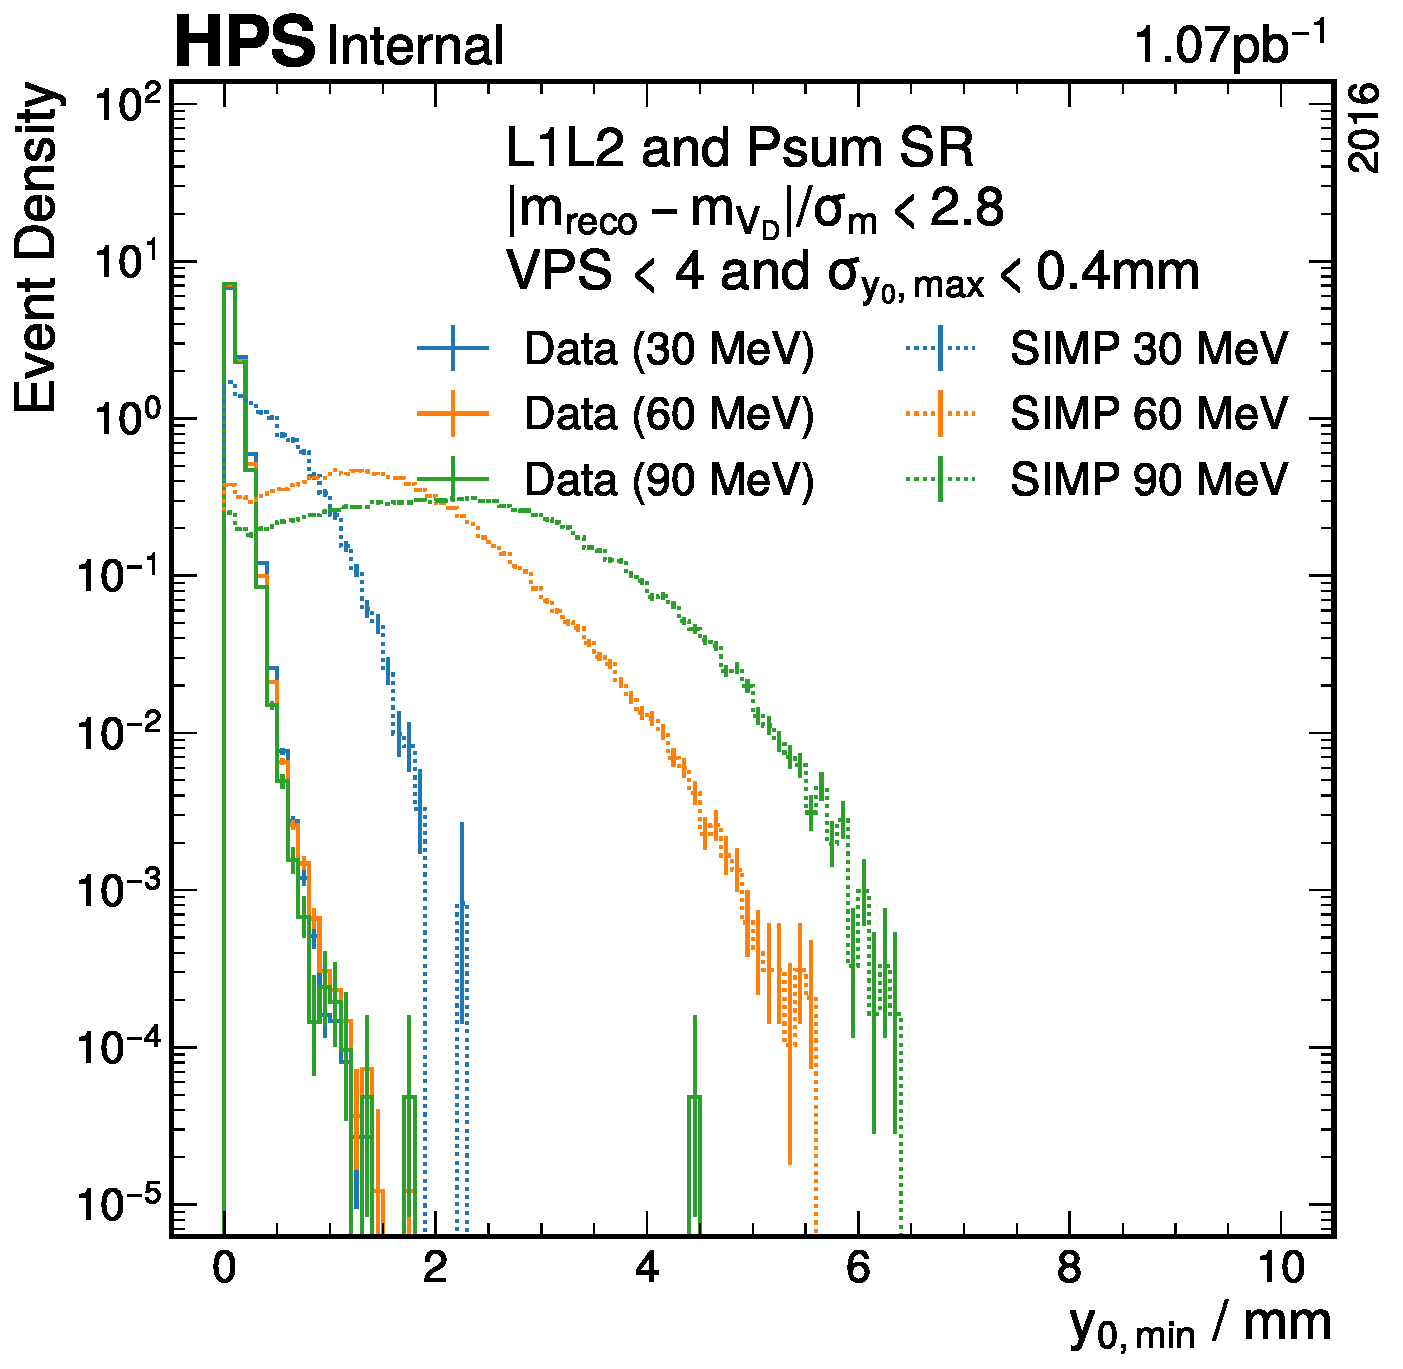
\includegraphics[width=\textwidth]{%
        ../figures/hps/analysis/min-y0-after-others.pdf}
      }
    \end{column}
    \begin{column}{0.69\textwidth}
      \begin{block}{Binomial Significance}
        Maximize binomial significance $Z_\mathrm{Bi}$
        within core mass region with best sensitivity
        and then smooth with a linear fit.
      \end{block}
      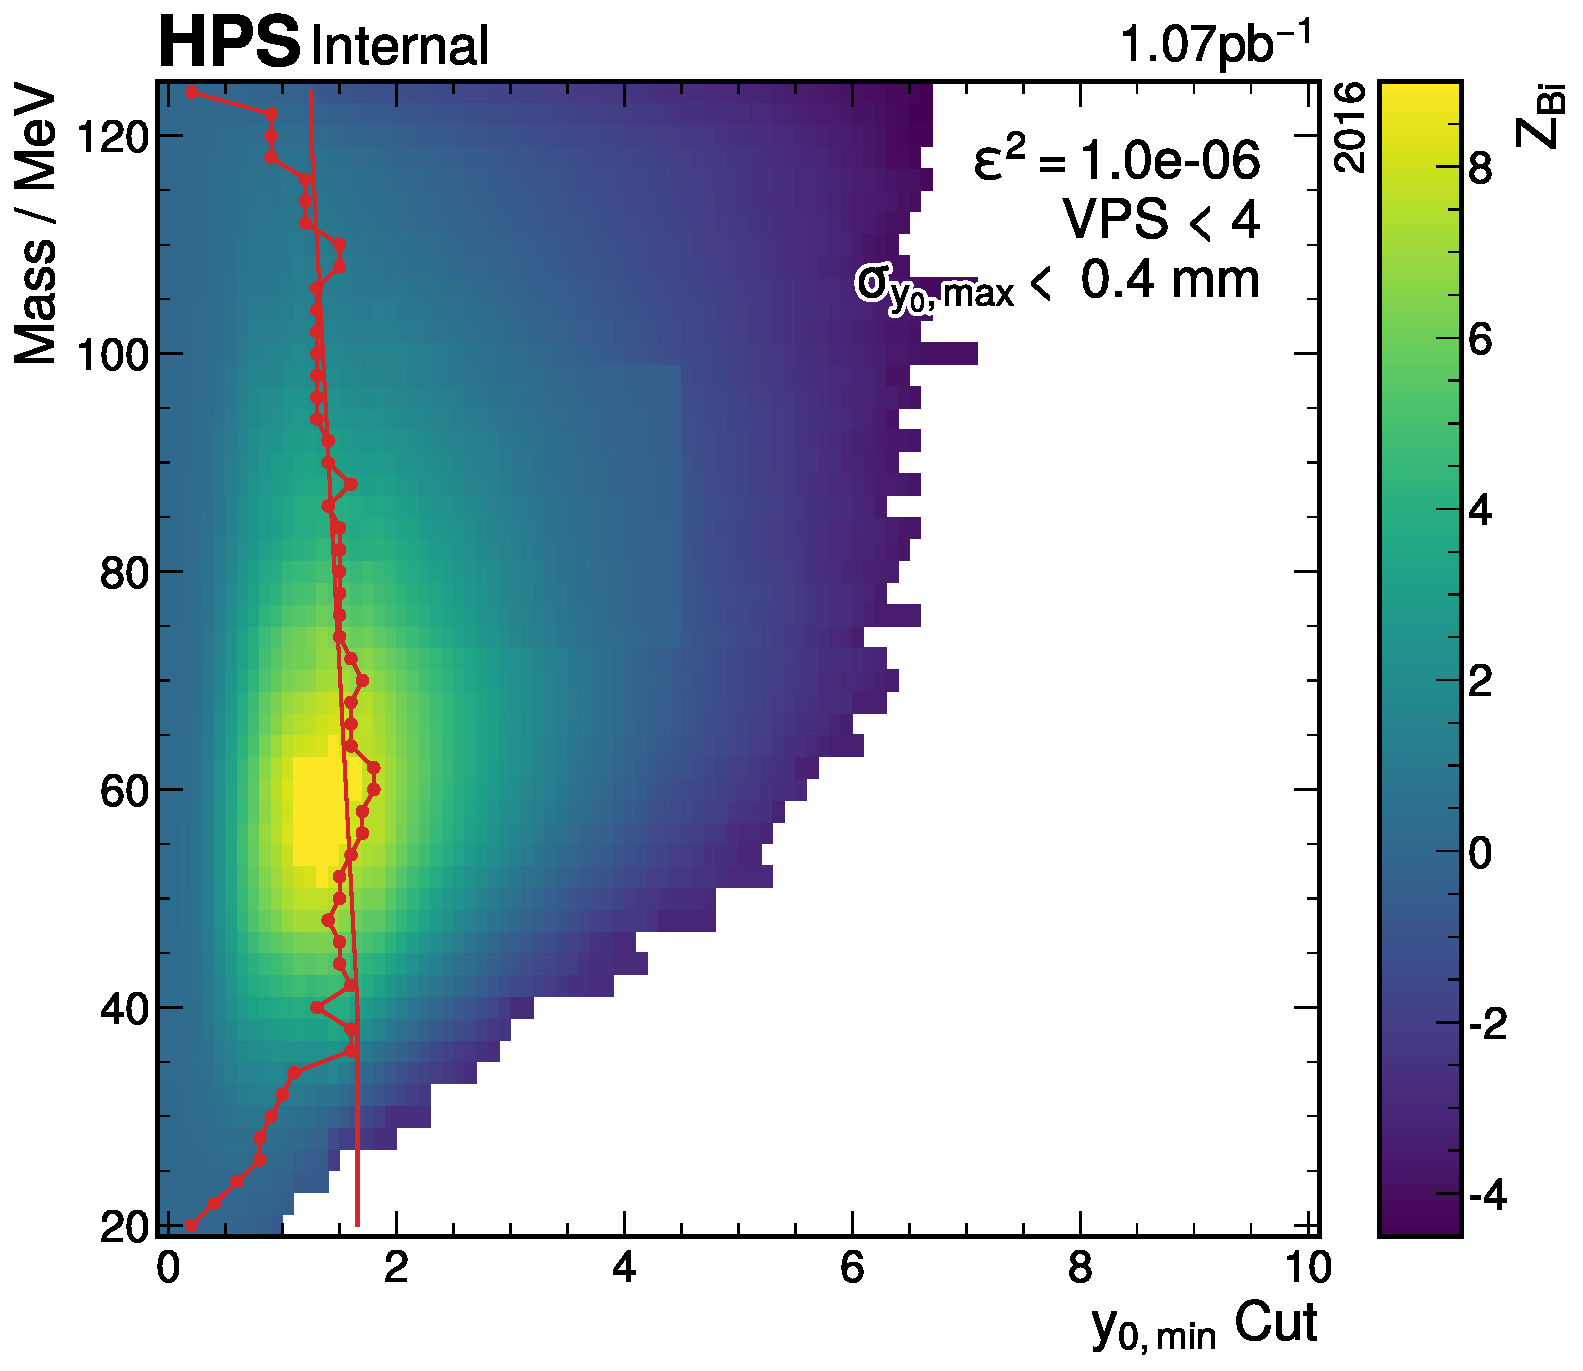
\includegraphics[width=0.48\textwidth]{%
        ../figures/hps/analysis/miny0-after-others-zbi-eps2-1e-6.pdf}
      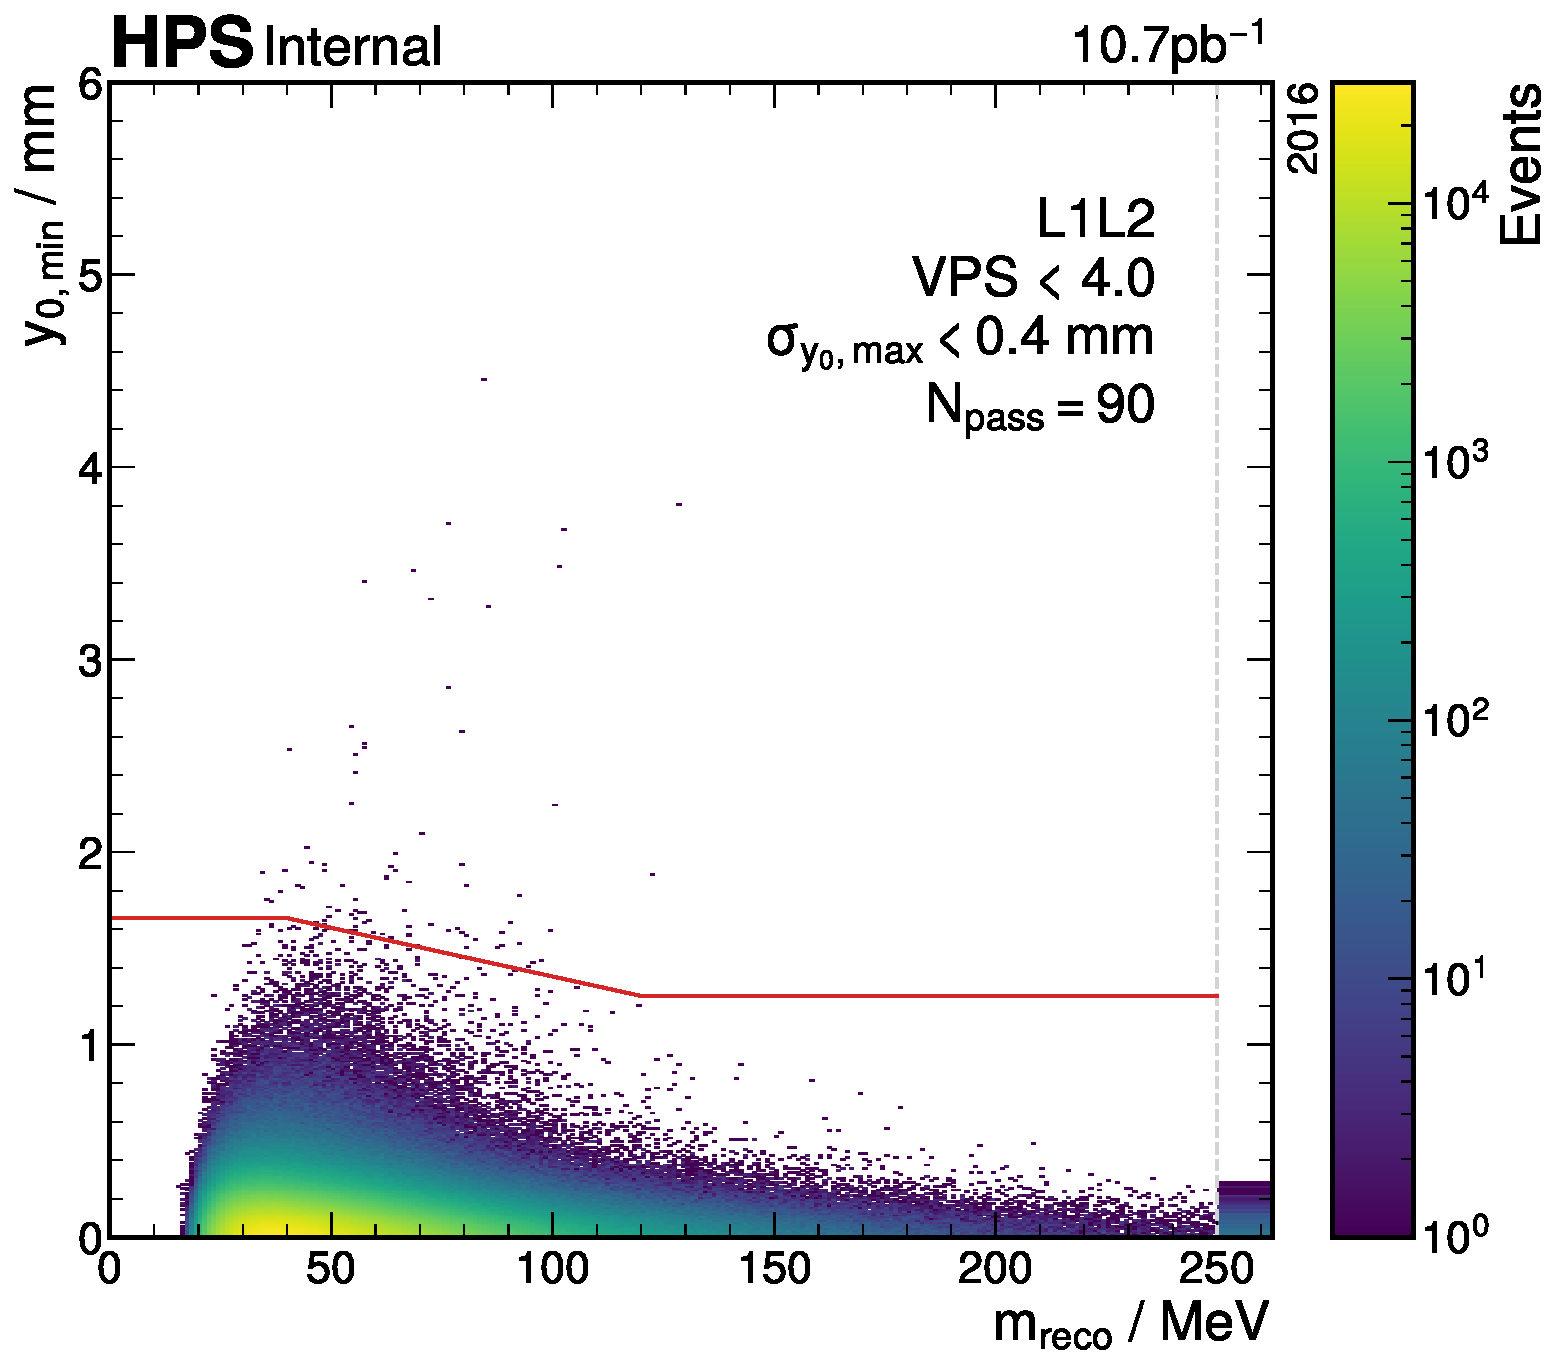
\includegraphics[width=0.48\textwidth]{%
        ../figures/hps/analysis/results/y0-cut-on-data.pdf}
    \end{column}
  \end{columns}
\end{frame}

\note[itemize]{
\item Trim the data tail of the \minyzero distribution while keeping the signal efficiency
  high
\item After some searching and double-checking, landed on \ac{vps} $< 4$
  and \maxyzeroerr$< \qty{0.4}{\mm}$
\item After these additional quality cuts, we then focus on maximizing the binomial
  significance of the hypothetical signal on top of the background distribution
  \begin{itemize}
    \item Signal yield needed to be artificially scaled so that it was on the same
      order of magnitude as the observed data
    \item Varying this scale did not alter the chosen cuts except in extreme cases
  \end{itemize}
\item The cuts maximizing the $Z_\mathrm{Bi}$ are then smoothed with a linear fit
  to help alleviate statistical bias
\item \minyzero cut extending outside of the fit range with a flat value
\item Unblind...
}

\subsection{Run 2 Results}

\begin{frame}{Search}
  \begin{columns}
    \begin{column}{0.45\textwidth}
      \centering
      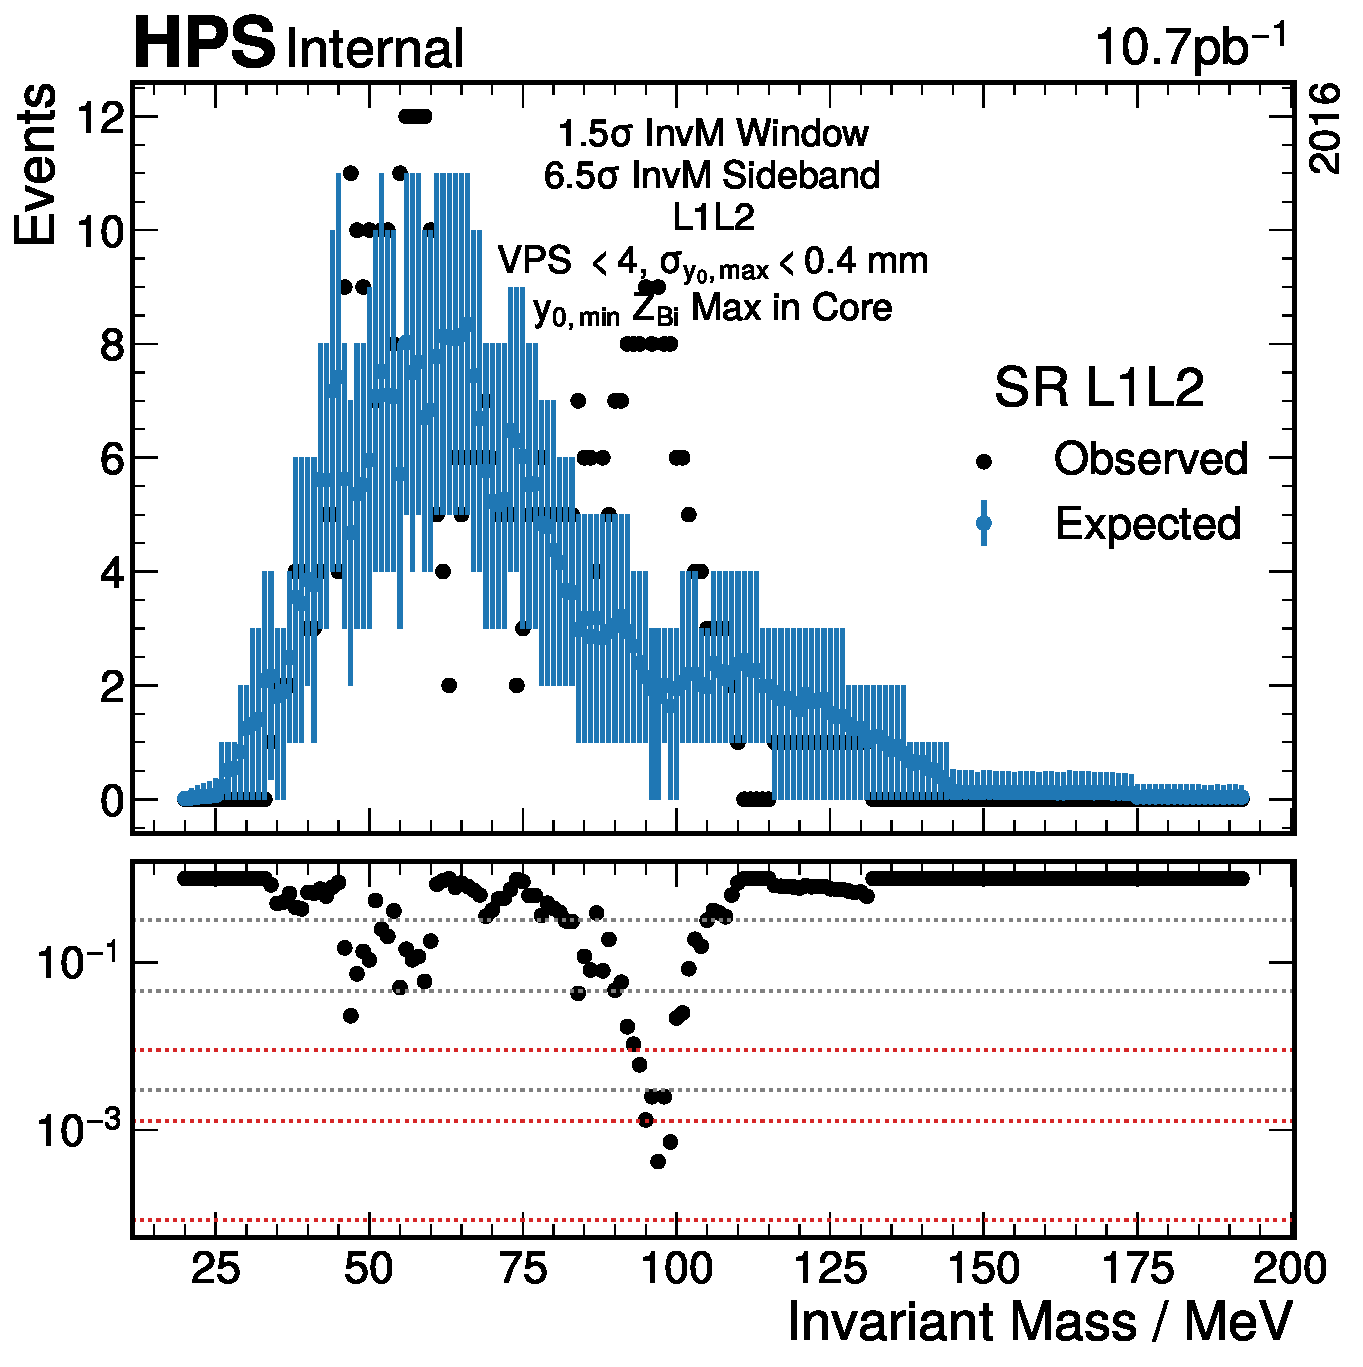
\includegraphics[width=\textwidth]{../figures/hps/analysis/results/search.pdf}
    \end{column}
    \begin{column}{0.55\textwidth}
      \centering
      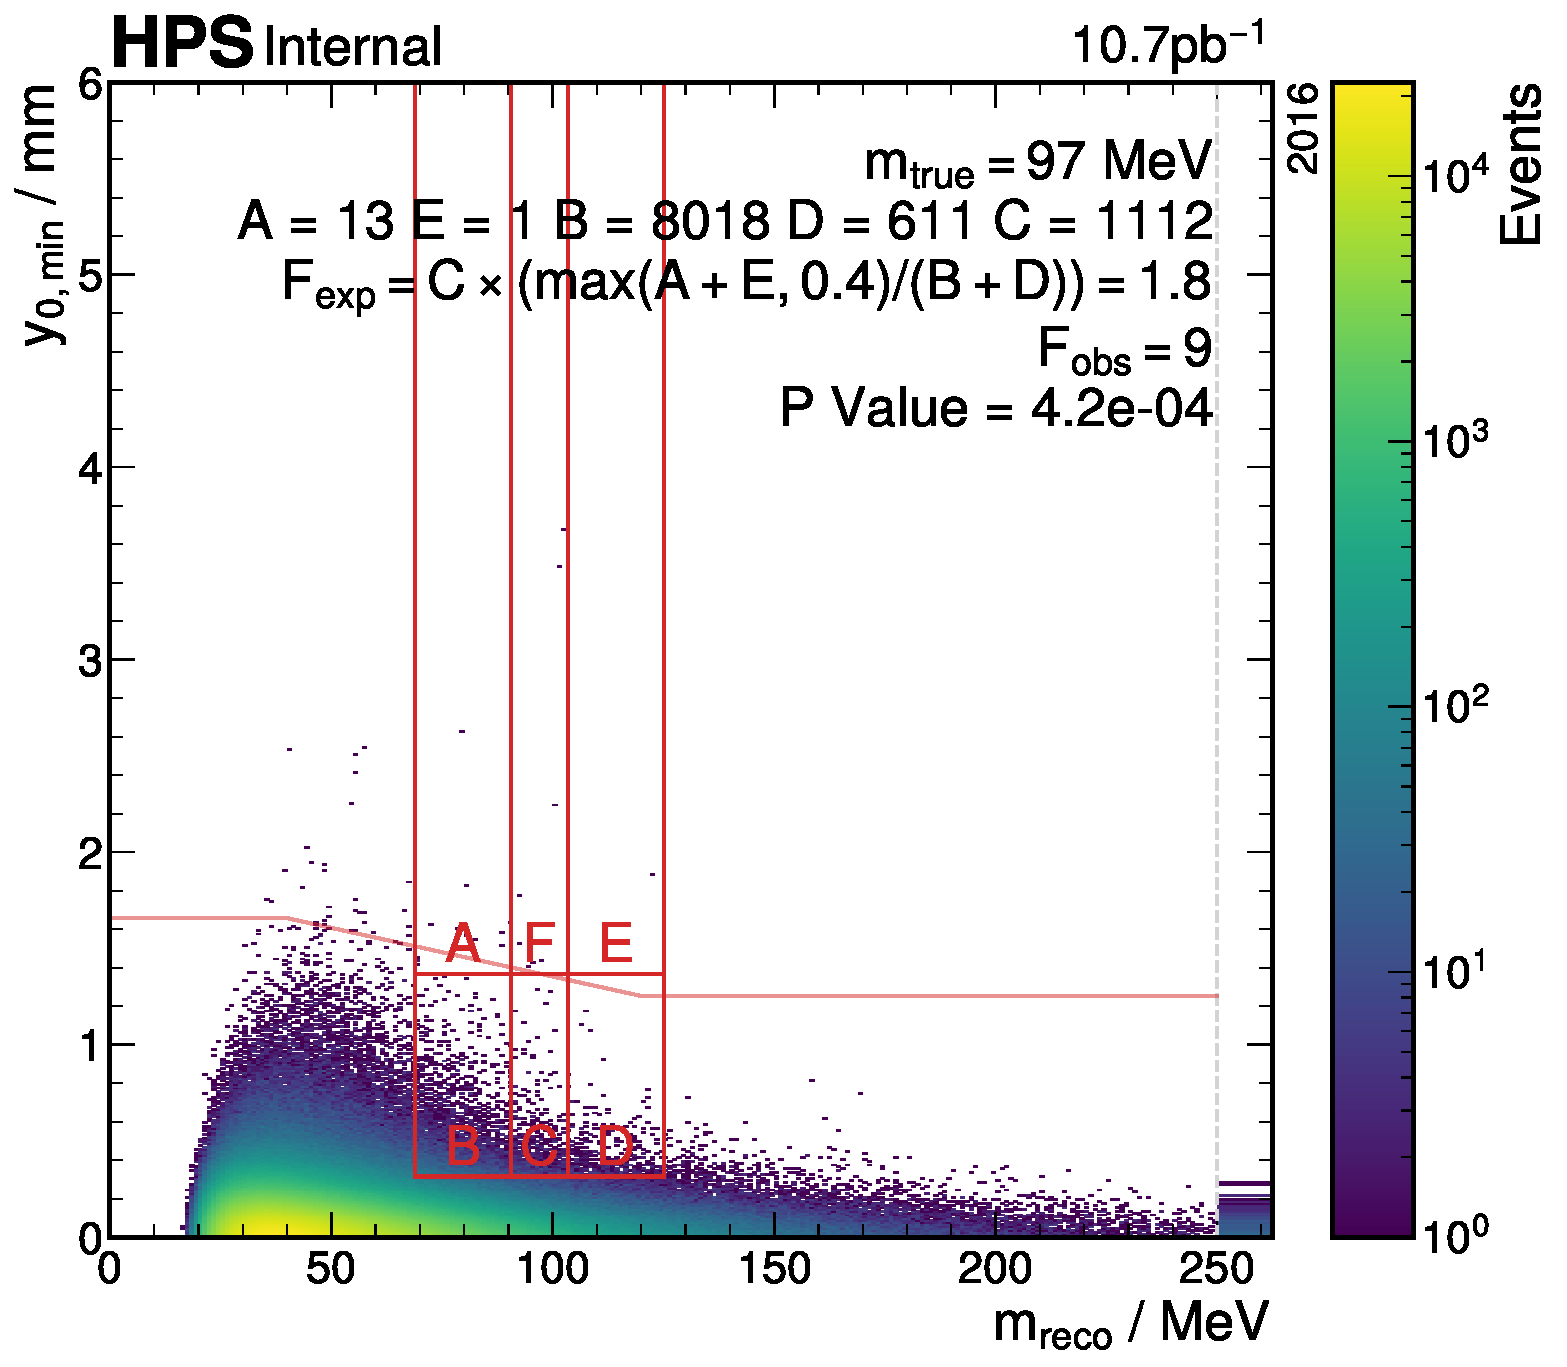
\includegraphics[width=\textwidth]{../figures/hps/analysis/results/search-min-p-val.pdf}
    \end{column}
  \end{columns}
\end{frame}

\note[itemize]{
\item Search for excess in mass-displacement space using a modified ABCD approach
\item Do not observe any excess exceeding one sigma global significance (red lines)
  within the 10\% subsample used for cut optimization
\item No excess $\to$ move to exclusion
}

\begin{frame}{Sensitivity from L1L2}
  \begin{columns}
    \begin{column}{0.5\textwidth}
      \centering
      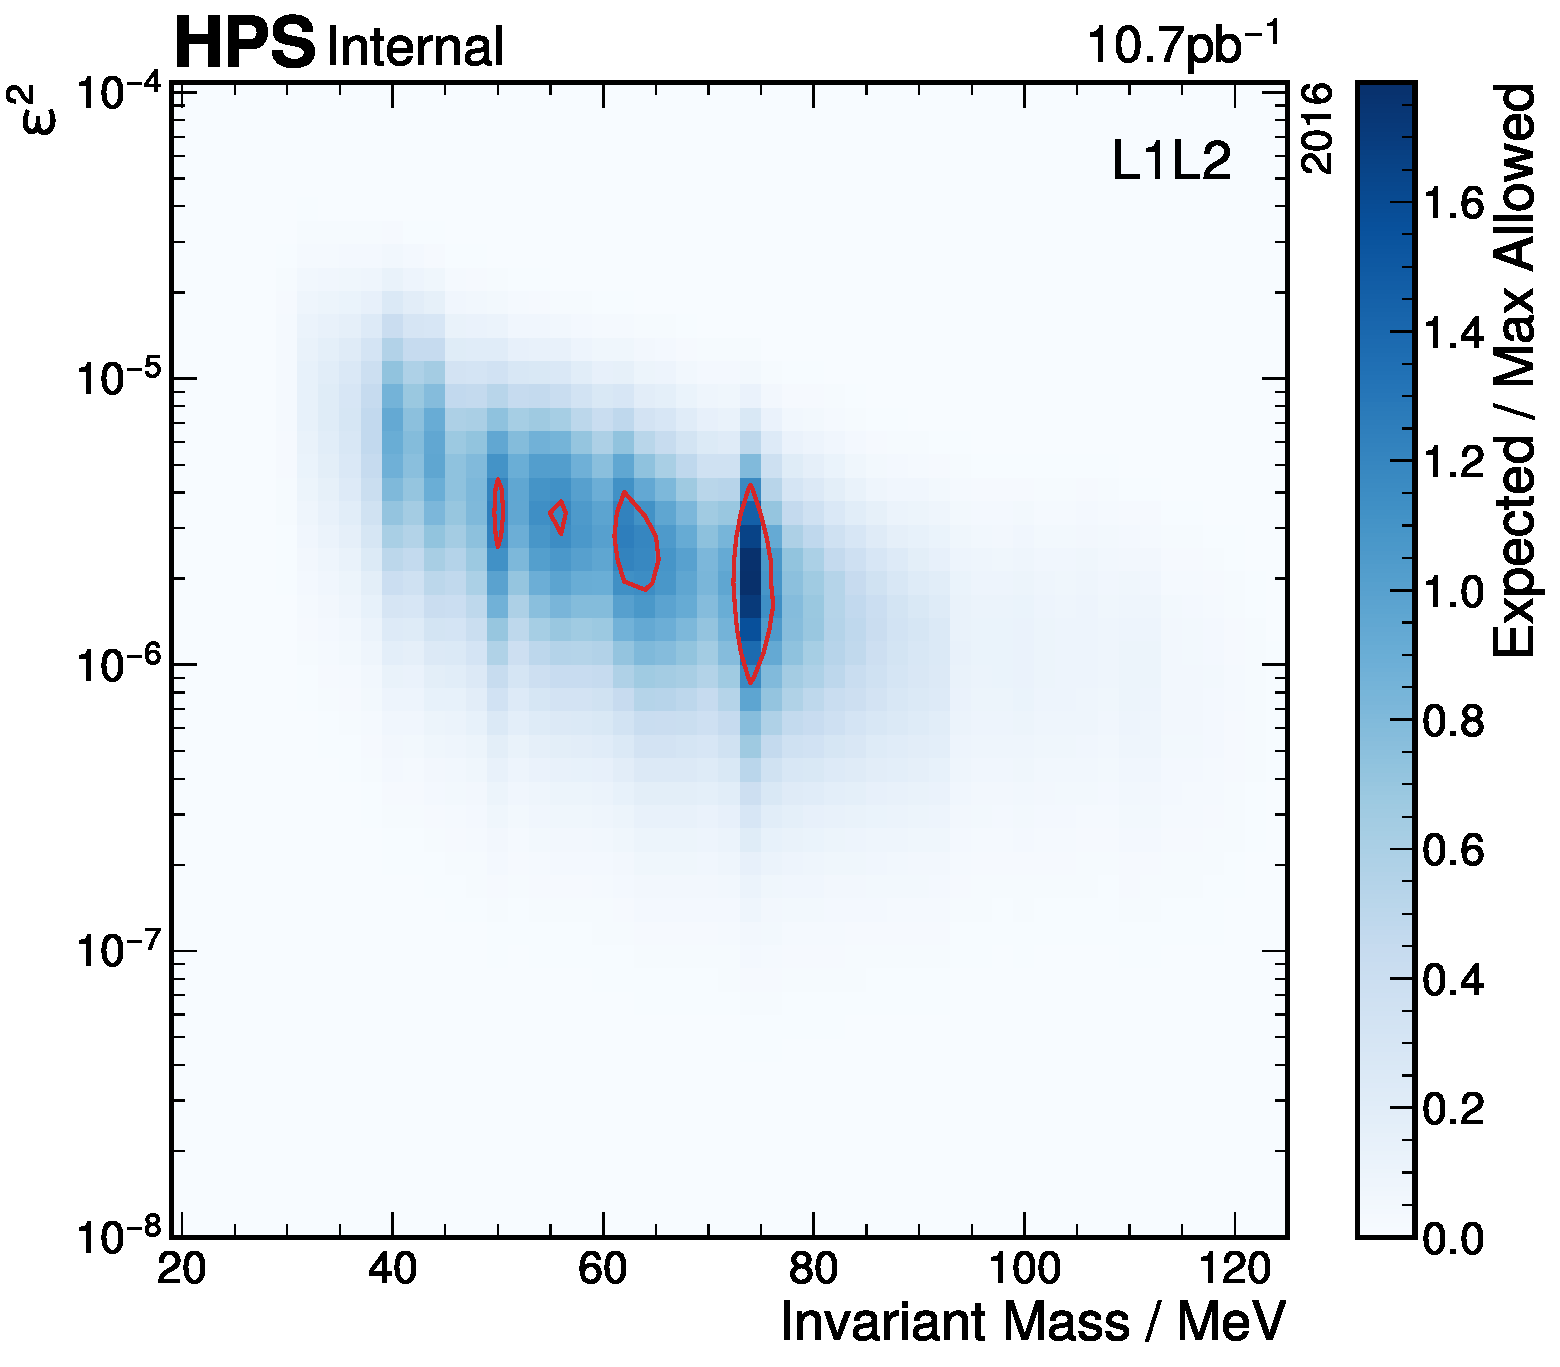
\includegraphics[width=\textwidth]{../figures/hps/analysis/results/exclusion-estimate.pdf}
    \end{column}
    \begin{column}{0.5\textwidth}
      \begin{itemize}
        \item No new exclusion on its own, but is able to re-exclude some parameters
        \item Combination with L1L1 results
          \begin{itemize}
            \item Extends exclusion below $\epsilon^2=10^{-6}$ line into new territory
          \end{itemize}
      \end{itemize}
      \begin{center}
        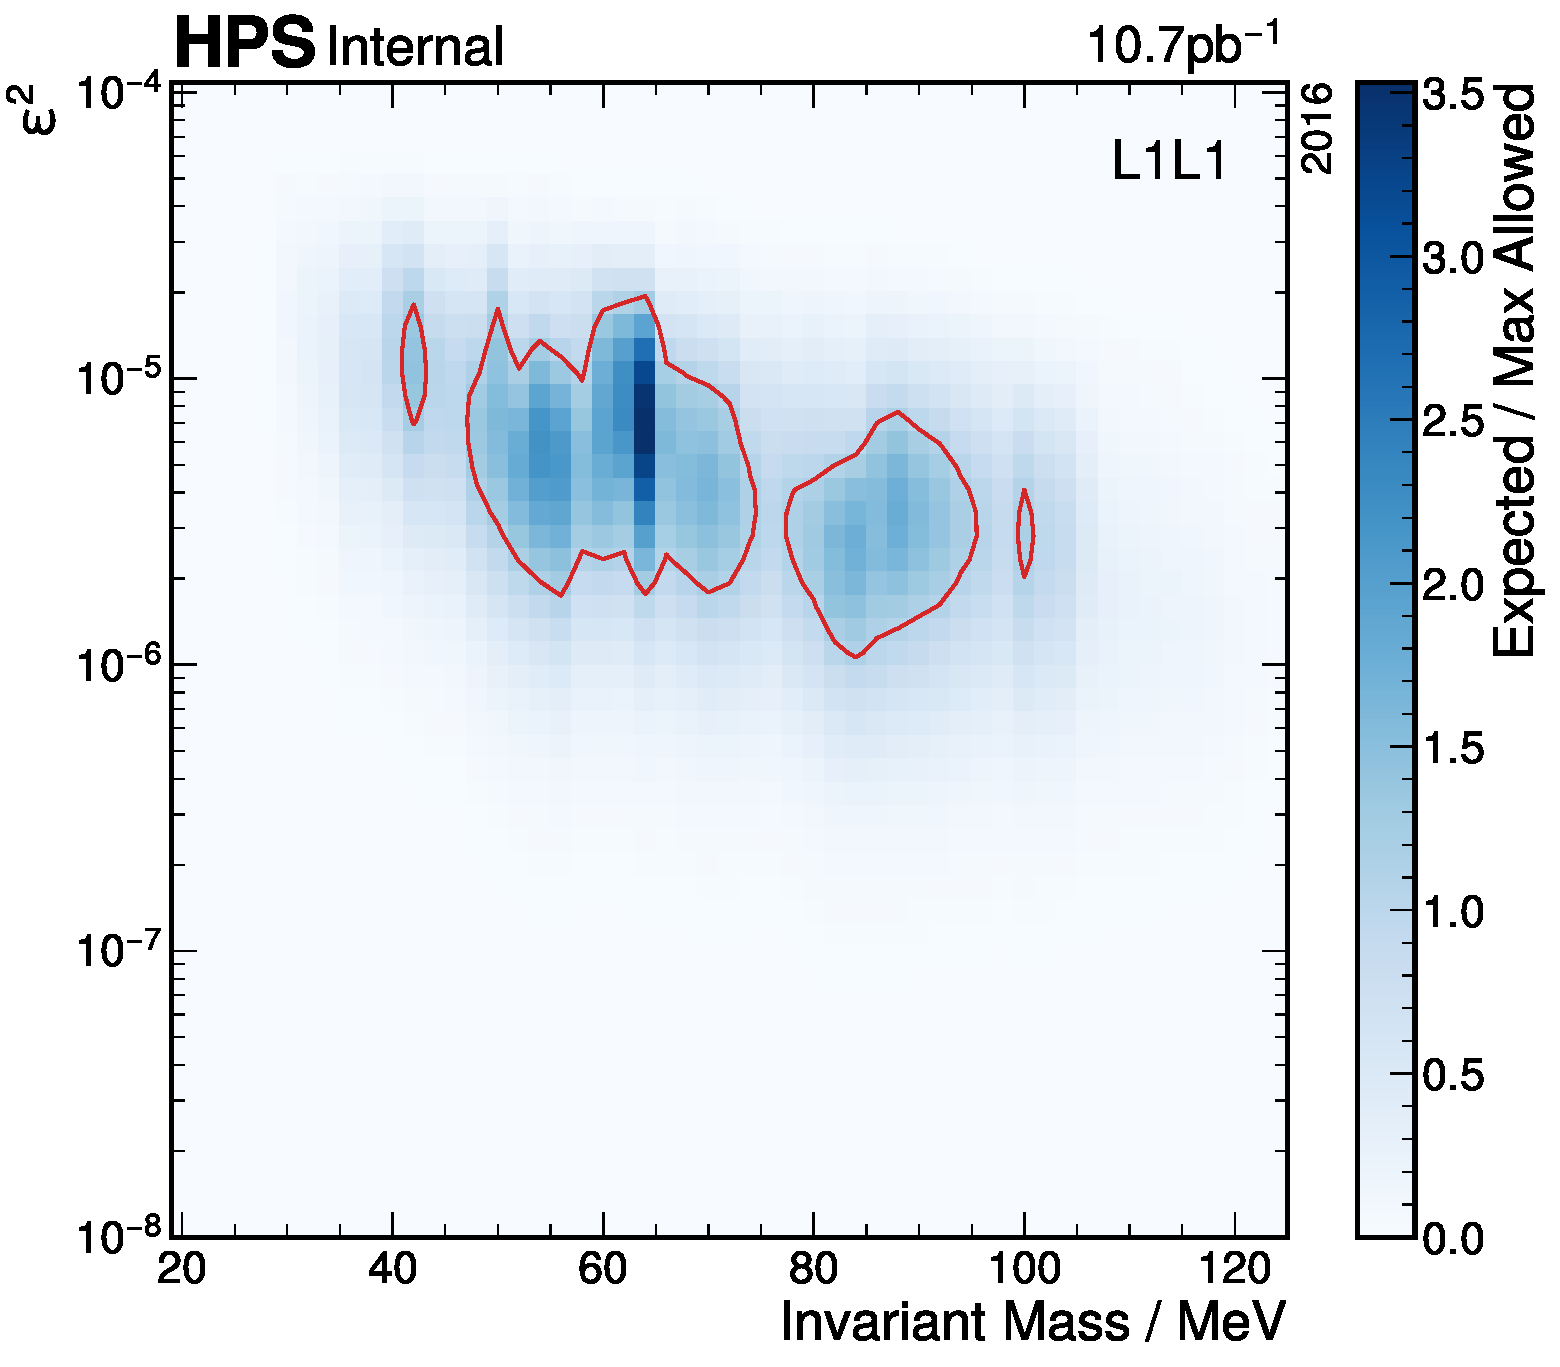
\includegraphics[height=0.4\textheight]{%
          ../figures/hps/analysis/results/l1l1-exclusion-estimate.pdf}
      \end{center}
    \end{column}
  \end{columns}
\end{frame}

\note[itemize]{
\item Calculate expected signal using SIMP model and use the \ac{oim}
  to estimate the maximum allowed signal yield
\item Ratio of these quantities gives the sensitivity of this analysis
\item Contour drawn where this value suppressed by systematic uncertainties is equal to 1
\item Combining this result with the L1L1 result solidifies the exclusion
  and lowers the contour in the core mass region
\item Contour Shape roughly made of three lines
  \begin{itemize}
    \item Bottom of triangle determined by data volume (are enough A' produced?)
    \item Top of triangle determined by decay length (does DM decay within HPS acceptance?)
    \item Left side determined by opening angle (smaller mass, more boost, pair more likely to go through central hole of HPS)
  \end{itemize}
}

\ssection{Looking Forward to Run 3}

\subsection{Dijet Mass Reweighting}

\subsection{2 vs. 3 Jet Studies}

\ssection{Conclusion}

\begin{frame}{Conclusion}
  Many ways to search for many types of \ac{dm}
  
  \begin{block}{LDMX}
    Missing momentum/energy search still in preparatory stages
  \end{block}

  \begin{block}{HPS}
    Excess highly-displaced events at specific mass searching within
    data for different \ac{dm} models
  \end{block}

  \begin{center}
    \color{UMNSunny}
    Both enable investigation of novel phase space
    in physics' quest to find \ac{dm}
  \end{center}
\end{frame}

\note{
  LDMX
  \begin{itemize}
    \item MM/ME search still in prepatory stages
    \item EaT work has helped prepare it for first data
  \end{itemize}

  HPS
  \begin{itemize}
    \item Displaced/resonant decay search
    \item This work has helped expand it to new DM models
  \end{itemize}

  Both analysis have forthcoming papers and both enable
  investigation of novel phase space
}

\begin{backup}

\begin{frame}{LDMX Midshower Simulation Samples}
  \begin{table}
    \begin{tabular}{|c|c|c|}
    \hline
    Sample & Biasing Factor & Biasing Threshold
    \\ \hline
    Signal & $m_A^{\max(\log_{10}(m_A),2))}/\epsilon^2$ & $0.5E_\text{Beam}$
    \\
    Enriched Nuclear & $200$ & $0.375E_\text{Beam}$
    \\
    Di-Muon & $10^5$ & $0.5E_\text{Beam}$
    \\
    \hline \hline
    Sample & \multicolumn{2}{c|}{Filtering Cuts}
    \\ \hline
    Unbiased  
        & \multicolumn{2}{c|}{$E_{\text{primary}}^{\text{ECal Front}} \geq 0.875E_\text{Beam}$}
    \\
    Signal 
        & \multicolumn{2}{c|}{$E_{\text{primary}}^{\text{ECal Front}} \geq 0.875E_\text{Beam}$ \& $E_{A'}\geq 0.5E_\text{Beam}$}
    \\
    Enriched Nuclear
        & \multicolumn{2}{c|}{$E_{\text{primary}}^{\text{ECal Front}} \geq 0.875E_\text{Beam}$ \& $E_{\text{tot nuc}}\geq 0.625E_\text{Beam}$}
    \\
    Di-Muon
        & \multicolumn{2}{c|}{$E_{\text{primary}}^{\text{ECal Front}} \geq 0.875E_\text{Beam}$ \& $E_{\text{tot}~\mu}\geq 0.5E_\text{Beam}$}
    \\ \hline
\end{tabular}

    \caption{Configuration of the simulation samples used in this analysis. $E_\mathrm{beam}$ is the beam energy being studied ($4$ or $8$ GeV in this work). $m_A$ is the mass of the A' in MeV, $\epsilon$ is the dark brem mixing strength, $E_{\text{primary}}^{\text{ECal Front}}$ is the energy of the primary electron at the front of the ECal, $E_{A'}$ is the energy of the generated A', $E_{\text{tot nuc}}$ is the total energy transferred to nuclear interactions during the event, and $E_{\text{tot}~\mu}$ is the total energy of produced muons.}
  \end{table}
\end{frame}

\begin{frame}{HPS Modified ABCD(EF) Search Method}
  \begin{columns}
    \begin{column}{0.5\textwidth}
      \centering
      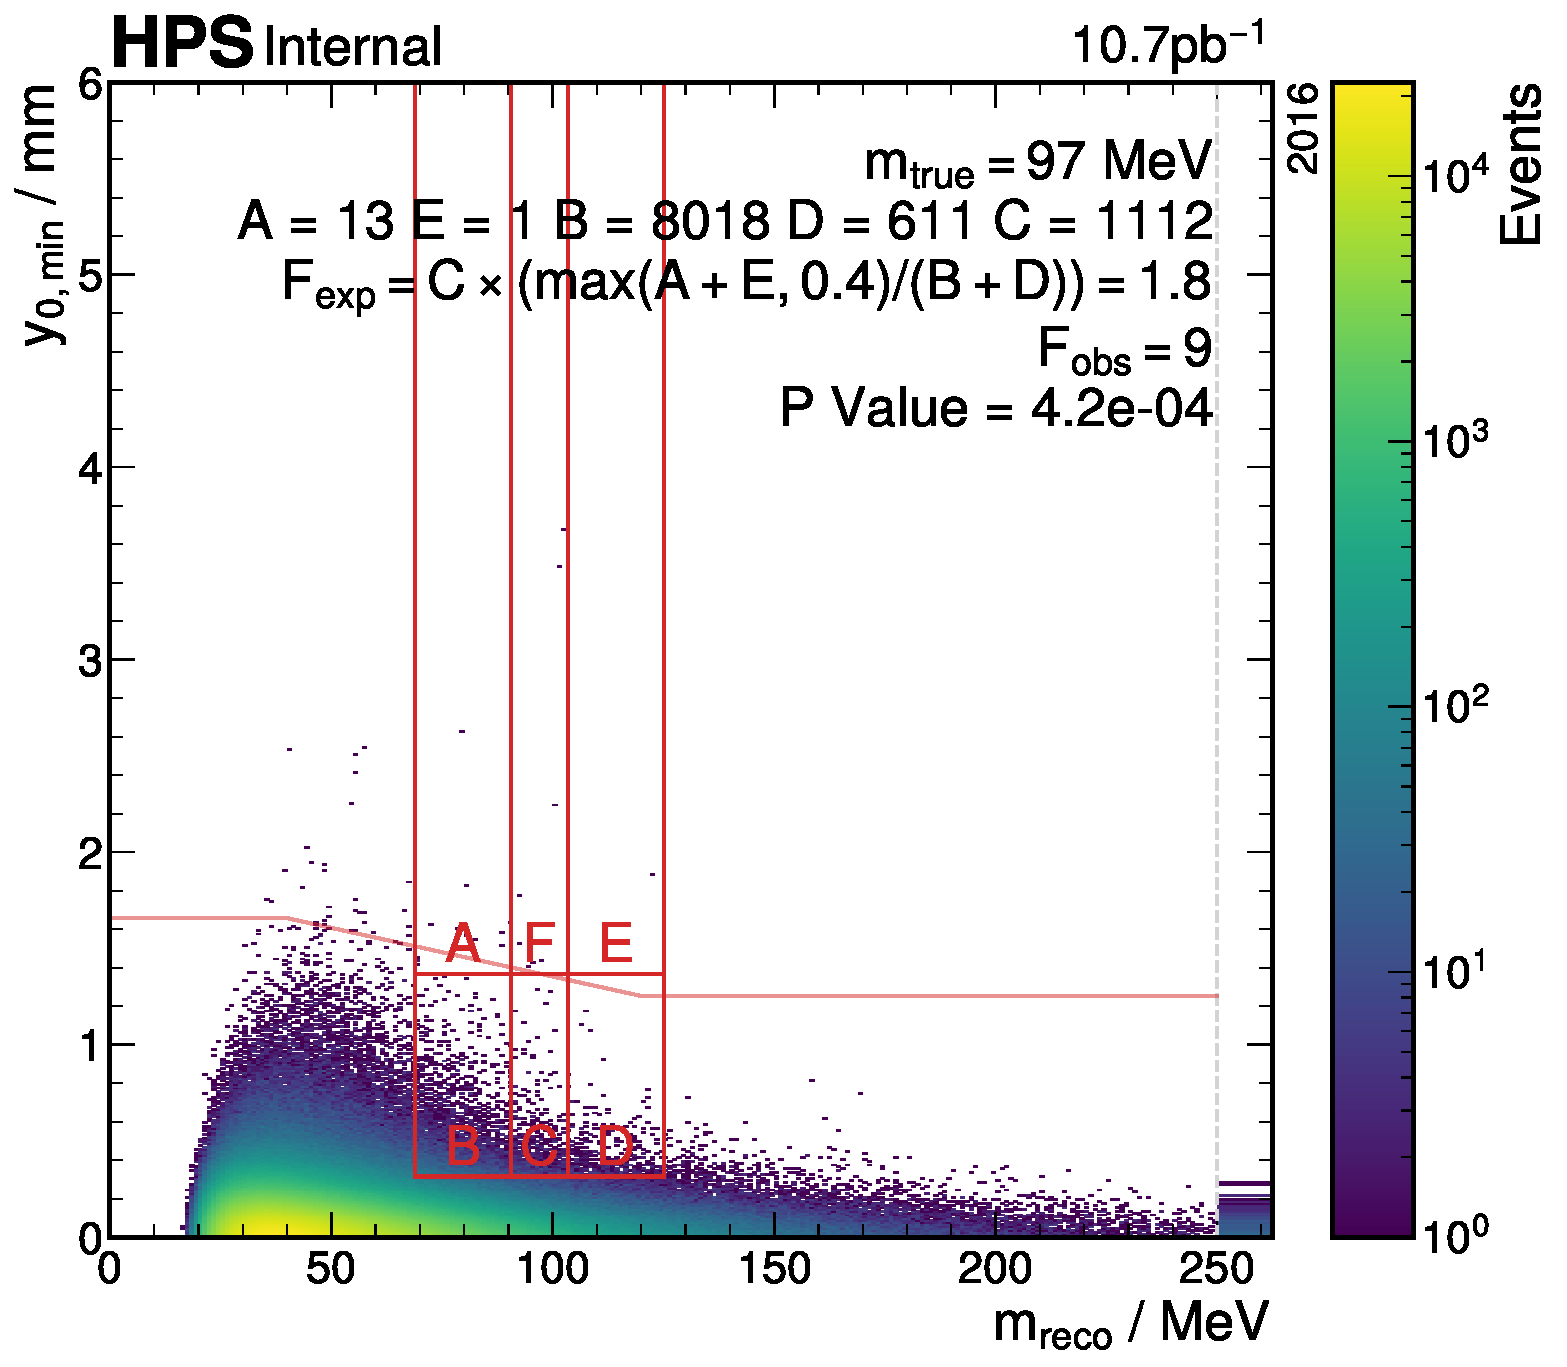
\includegraphics[width=\textwidth]{../figures/hps/analysis/results/search-min-p-val.pdf}
    \end{column}
    \begin{column}{0.5\textwidth}
      \begin{enumerate}
        \item Fill histogram with data
        \item Set mass edges at $1.5\sigma$ and $4.5\sigma$ (values optimized by A Spellmen)
        \item Set upper \minyzero edge at cut value
        \item Lower other \minyzero edge (a.k.a. $y_0$ ``floor'') from the cut value
          until there are at least 1k events in region C
        \item Calculate expected number of events in F
          and compare to observed number of events
        \item Estimate p-value by throwing toy experiments in A+E (Poission), B+D
          and C (Normal) and re-calculating F from these toys
      \end{enumerate}
    \end{column}
  \end{columns}
\end{frame}

\end{backup}

\end{document} 
